%------------------------------------------------------------------------------
%    POLITECNICO DI MILANO - THESIS TEMPLATE
%------------------------------------------------------------------------------
\documentclass{Configuration_Files/PoliMi3i_thesis}

%------------------------------------------------------------------------------
%	REQUIRED PACKAGES AND CONFIGURATIONS
%------------------------------------------------------------------------------

% CONFIGURATIONS
\usepackage{parskip} % For paragraph layout
\usepackage{setspace} % For using single or double spacing
\usepackage{emptypage} % To insert empty pages
\usepackage{multicol} % To write in multiple columns (executive summary)
\setlength\columnsep{15pt} % Column separation in executive summary
\setlength\parindent{0pt} % Indentation
\raggedbottom

% PACKAGES FOR TITLES
\usepackage{titlesec}
\titlespacing{\section}{0pt}{3.3ex}{2ex}
\titlespacing{\subsection}{0pt}{3.3ex}{1.65ex}
\titlespacing{\subsubsection}{0pt}{3.3ex}{1ex}
\usepackage{color}

% PACKAGES FOR LANGUAGE AND FONT
\usepackage[english]{babel} % The document is in English
\usepackage[utf8]{inputenc} % UTF8 encoding
\usepackage[T1]{fontenc} % Font encoding
\usepackage[11pt]{moresize} % Big fonts

% PACKAGES FOR IMAGES
\usepackage{graphicx}
\usepackage{transparent} % Enables transparent images
\usepackage{eso-pic} % For the background picture on the title page
\usepackage{subfig} % Numbered and caption subfigures using \subfloat
\usepackage{tikz} % A package for high-quality hand-made figures
\usetikzlibrary{}
\graphicspath{{./Images/}} % Directory of the images
\usepackage{caption} % Coloured captions
\usepackage{xcolor} % Coloured captions
\usepackage{amsthm,thmtools,xcolor} % Coloured "Theorem"
\usepackage{float}

% STANDARD MATH PACKAGES
\usepackage{amsmath}
\usepackage{amsthm}
\usepackage{amssymb}
\usepackage{amsfonts}
\usepackage{bm}
\usepackage[overload]{empheq} % For braced-style systems of equations
\usepackage{fix-cm} % To override original LaTeX restrictions on sizes

% PACKAGES FOR TABLES
\usepackage{tabularx}
\usepackage{longtable} % Tables that can span several pages
\usepackage{colortbl}

% PACKAGES FOR ALGORITHMS (PSEUDO-CODE)
\usepackage{algorithm}
\usepackage{algorithmic}

% PACKAGES FOR REFERENCES & BIBLIOGRAPHY
\usepackage[colorlinks=true, linkcolor=black, anchorcolor=black, citecolor=black, filecolor=black, menucolor=black, 
            runcolor=black, urlcolor=black]{hyperref} % Adds clickable links at references
\usepackage{cleveref}
\usepackage[square, numbers, sort&compress]{natbib} % Square brackets, citing references with numbers, citations sorted 
                                                    % by appearance in the text and compressed
\bibliographystyle{abbrvnat} % You may use a different style adapted to your field

% OTHER PACKAGES
\usepackage{pdfpages} % To include a pdf file
\usepackage{afterpage}
\usepackage{lipsum} % DUMMY PACKAGE
\usepackage{fancyhdr} % For the headers
\usepackage{pdflscape} % For landscape pages
\fancyhf{}

% CONFIGURATION FILE
% Define blue color typical of polimi
\definecolor{bluepoli}{cmyk}{0.4,0.1,0,0.4}

% Custom theorem environments
\declaretheoremstyle[
  headfont=\color{bluepoli}\normalfont\bfseries,
  bodyfont=\color{black}\normalfont\itshape,
]{colored}

% Set-up caption colors
\captionsetup[figure]{labelfont={color=bluepoli}} % Set colour of the captions
\captionsetup[table]{labelfont={color=bluepoli}} % Set colour of the captions
\captionsetup[algorithm]{labelfont={color=bluepoli}} % Set colour of the captions

\theoremstyle{colored}
\newtheorem{theorem}{Theorem}[chapter]
\newtheorem{proposition}{Proposition}[chapter]

% Enhances the features of the standard "table" and "tabular" environments.
\newcommand\T{\rule{0pt}{2.6ex}}
\newcommand\B{\rule[-1.2ex]{0pt}{0pt}}

% Pseudo-code algorithm descriptions.
\newcounter{algsubstate}
\renewcommand{\thealgsubstate}{\alph{algsubstate}}
\newenvironment{algsubstates}
{\setcounter{algsubstate}{0}%
  \renewcommand{\STATE}{%
    \stepcounter{algsubstate}%
    \Statex {\small\thealgsubstate:}\space}}
{}

% New font size
\newcommand\numfontsize{\@setfontsize\Huge{200}{60}}

% Title format: chapter
\titleformat{\chapter}[hang]{
  \fontsize{50}{20}\selectfont\bfseries\filright}{\textcolor{bluepoli} \thechapter\hsp\hspace{2mm}\textcolor{bluepoli}{|   }\hsp}{0pt}{\huge\bfseries \textcolor{bluepoli}
}

% Title format: section
\titleformat{\section}
{\color{bluepoli}\normalfont\Large\bfseries}
{\color{bluepoli}\thesection.}{1em}{}

% Title format: subsection
\titleformat{\subsection}
{\color{bluepoli}\normalfont\large\bfseries}
{\color{bluepoli}\thesubsection.}{1em}{}

% Title format: subsubsection
\titleformat{\subsubsection}
{\color{bluepoli}\normalfont\large\bfseries}
{\color{bluepoli}\thesubsubsection.}{1em}{}

% Shortening for setting no horizontal-spacing
\newcommand{\hsp}{\hspace{0pt}}

\makeatletter
% Renewcommand: cleardoublepage including the background pic
\renewcommand*\cleardoublepage{%
  \clearpage\if@twoside\ifodd\c@page\else
      \null
      \AddToShipoutPicture*{\BackgroundPic}
      \thispagestyle{empty}%
      \newpage
      \if@twocolumn\hbox{}\newpage\fi\fi\fi}
\makeatother

%For correctly numbering algorithms
\numberwithin{algorithm}{chapter}

%----------------------------------------------------------------------------
%	STARTING POINT OF THE DOCUMENT
%----------------------------------------------------------------------------
\begin{document}

\fancypagestyle{plain}{%
    \fancyhf{} % Clear all header and footer fields
    \fancyhead[RO,RE]{\thepage} % RO=right odd, RE=right even
    \renewcommand{\headrulewidth}{0pt}
    \renewcommand{\footrulewidth}{0pt}}

%----------------------------------------------------------------------------
%	TITLE PAGE
%----------------------------------------------------------------------------
\pagestyle{empty} % No page numbers
\frontmatter % Use roman page numbering style (i, ii, iii, iv...) for the preamble pages

\puttitle{
    documentTitle = Students\&Companies: \\ Design Document (DD),
    course = Software Engineering II,
    authorOne = Marco Apollonio (10764083),
    authorTwo = Giacomo Bossi (10766073),
    authorThree = Lorenzo Chiroli (10797603),
    advisor= Prof.ssa. Elisabetta Di Nitto,
    academicYear= 2024-2025
}

%----------------------------------------------------------------------------
%	LIST OF CONTENTS/FIGURES/TABLES/SYMBOLS
%----------------------------------------------------------------------------
\startpreamble
\setcounter{page}{1} % Set page counter to 1
\thispagestyle{empty} % No page numbers on this page
\tableofcontents % Write out the Table of Contents
\thispagestyle{empty} % No page numbers on this page
\cleardoublepage % Start the document on a right-hand page

%-------------------------------------------------------------------------
%	DOCUMENT MAIN TEXT
%-------------------------------------------------------------------------
\addtocontents{toc}{\vspace{2em}} % Add a gap in the Contents, for aesthetics
\mainmatter % Begin numeric (1,2,3...) page numbering

\chapter{Introduction}
\label{ch:introduction}% 
% The \label{...}% enables to remove the small indentation that is generated, always leave the % symbol.

\par In today's rapidly evolving job market, there is a growing concern regarding the skill mismatch between fresh
graduates and the requirements of employers. This issue is particularly prevalent in the realm of internships,
especially in the STEM field, where students are often not able to meet the demands of industry-relevant roles, while
companies struggle to find candidates with the necessary skills for their internship programs.

\par This skill mismatch not only harms the career development of students but also affects the productivity of the
companies themselves. On one hand, students miss out on valuable learning opportunities and real-world experiences. On
the other hand, companies experience inefficiencies due to the time and resources spent on training interns who lack
the essential skills required for their roles.

\par To address this issue, we wish to establish a platform that connects students with relevant internship
opportunities while simultaneously providing employers with a pool of qualified candidates. S\&C also aims to empower
universities to take a proactive role in resolving potential issues that may arise between students and companies, thus
creating a safe space for both parties.

\section{Purpose}
\label{sec:purpose}%

\par This document serves mainly as a comprehensive reference for the development team involved in implementing
Students\&Companies.

\par This material also aims to provide an authoritative overview of the software's capabilities and constraints,
ensuring clear understanding among all stakeholders: students, companies, and university personnel.

\subsection{Goals}
\label{subsec:goals}%

\begin{longtable}{|l|p{0.9\textwidth}|}
    \hline
    \textbf{Goal} & \textbf{Description}                                                                                                                              \\
    \hline \hline
    \multicolumn{2}{|l|}{\textit{From a student perspective...}}                                                                                                      \\
    \hline
    G01           & Allow the ST to login using the UN-provided credentials.                                                                                          \\
    \hline
    G02           & Allow the ST to upload their own CV on the platform.                                                                                              \\
    \hline
    G03           & Allow the ST to see the internships published by the various COs.                                                                                 \\
    \hline
    G04           & Allow the ST to receive suggestions about internships that he might be interested in.                                                             \\
    \hline
    G05           & Allow the ST to apply for an internship.                                                                                                          \\
    \hline
    G06           & Allow the ST to fill out the interview questionnaires sent by the COs.                                                                            \\
    \hline
    G07           & Allow the ST to be contacted directly by the COs in order to start the internship (if they wish so).                                              \\
    \hline
    G08           & Allow the ST to complain if any problems occur during the internship itself.                                                                      \\
    \hline
    G09           & Allow the ST to give feedback after the internship is done.                                                                                       \\
    \hline
    G10           & Allow the ST to see a checklist with recommendations on how to make their CV better.                                                              \\
    \hline
    G11           & Allow the ST to be informed on the status of their own internships.                                                                               \\
    \hline \hline
    \multicolumn{2}{|l|}{\textit{From a company perspective...}}                                                                                                      \\
    \hline
    G12           & Allow the CO to login using the provided (after-sale) credentials.                                                                                \\
    \hline
    G13           & Allow the CO to edit their own CO profile (public, visible to STs and UNs).                                                                       \\
    \hline
    G14           & Allow the CO to publish an internship announcement.                                                                                               \\
    \hline
    G15           & Allow the CO to receive CV suggestions corresponding to its needs and asks these people to apply for the internships.                             \\
    \hline
    G16           & Allow the CO to see applications and selected them to proceed with the questionnaire compilations by the STs.                                     \\
    \hline
    G17           & Allow the CO to see the questionnaire results to choose STs to contact.                                                                           \\
    \hline
    G18           & Allow the CO to update the internship status (by also specifying who is taking to work with) by also adding comments if necessary during the job. \\
    \hline
    G19           & Allow the CO to complain if any problems occur during the internship itself.                                                                      \\
    \hline
    G20           & Allow the CO to see a checklist with recommendations on how to make their internship announcement better.                                         \\
    \hline
    G21           & Allow the CO to be informed on the status of their own internships.                                                                               \\
    \hline \hline
    \multicolumn{2}{|l|}{\textit{From a university perspective...}}                                                                                                   \\
    \hline
    G22           & Allow the UN to login using the provided (after-sale) credentials.                                                                                \\
    \hline
    G23           & Allow the UN to see the complaints and make proactive decisions about them.                                                                       \\
    \hline
    G24           & Allow the UN to fully monitor the status and outcome of all past and present internships.                                                         \\
    \hline
    \caption{S\&C Goals Table}
    \label{tab:goals}
\end{longtable}

\section{Scope}
\label{sec:scope}%

\par S\&C is a platform that matches students seeking internships with companies offering these opportunities. The
platform manages internship postings and student applications, while allowing companies to evaluate candidates through
customized questionnaires. Throughout the internship, both parties can provide feedback on its progress, with
universities mediating any disputes that arise.

\par The platform employs recommendation algorithms to suggest relevant internship opportunities to students based on
their skills, while helping companies discover potential candidates that match their requirements.

\subsection{World Phenomena}
\label{subsec:world-phenomena}%

\begin{longtable}{|l|p{0.8\textwidth}|}
    \hline
    \textbf{Phenomena} & \textbf{Description}                                                                \\
    \hline \hline
    WP01               & STs build their own CVs.                                                            \\
    \hline
    WP02               & COs organize and manage their own internships.                                      \\
    \hline
    WP03               & COs plan the questions for the questionnaire they want to submit to the STs.        \\
    \hline
    WP04               & COs make contact with the eligible STs according to the questionnaire results.      \\
    \hline
    WP05               & STs take part in the internship if they've been selected by the CO.                 \\
    \hline
    WP06               & The CO contacts the S\&C sales team if they want to be enrolled in the application. \\
    \hline
    WP07               & UNs contact the S\&C sales team if they want to be enrolled in the application.     \\
    \hline
    \caption{World Phenomena Table}
    \label{tab:world-phenomena}
\end{longtable}

\subsection{Shared Phenomena}
\label{subsec:shared-phenomena}%

\begin{longtable}{|l|p{0.5\textwidth}|l|l|}
    \hline
    \textbf{Phenomena} & \textbf{Description}                                                                                                                                                                                                                                  & \textbf{Controller} & \textbf{Observer} \\
    \hline \hline
    SP01               & STs upload or modify their CVs on the platform.                                                                                                                                                                                                       & ST                  & S\&C              \\
    \hline
    SP02               & Each CV uploaded to S\&C is saved and processed by the CV analyzer, which will perform a feature extraction analysis. After the inspection, the owner of the document can see some suggestions on how to improve it.                                  & S\&C                & ST                \\
    \hline
    SP03               & STs look for interesting internships on the platform.                                                                                                                                                                                                 & ST                  & S\&C              \\
    \hline
    SP04               & The machine informs the users about relevant internships by sending a notification via email.                                                                                                                                                         & S\&C                & ST                \\
    \hline
    SP05               & STs apply for internships on the platform.                                                                                                                                                                                                            & ST                  & S\&C              \\
    \hline
    SP06               & STs complete the questionnaire for an internship.                                                                                                                                                                                                     & ST                  & S\&C              \\
    \hline
    SP07               & The machine assesses the questionnaire responses according to specified CO-provided criteria.                                                                                                                                                         & S\&C                & CO                \\
    \hline
    SP08               & If any problems occur during the internship, the STs can send a feedback report.                                                                                                                                                                      & ST                  & S\&C              \\
    \hline
    SP09               & The platform will forward internship feedback to the UN: a notification will be sent via email, and the UN can review them on S\&C.                                                                                                                   & S\&C                & UN                \\
    \hline
    SP10               & The S\&C sales team enrolls a CO on the platform. A set of unique credentials is created.                                                                                                                                                             & S\&C                & CO                \\
    \hline
    SP11               & COs edit their public profiles on S\&C.                                                                                                                                                                                                               & CO                  & S\&C              \\
    \hline
    SP12               & COs publish internship ads on S\&C.                                                                                                                                                                                                                   & CO                  & S\&C              \\
    \hline
    SP13               & Each internship post is analyzed and indexed. After the analysis, the CO can see suggestions on how to improve the copy.                                                                                                                              & S\&C                & CO                \\
    \hline
    SP14               & The machine sends to the COs CVs of relevant STs (matching the requirements of published internship ads or keywords on the matching CO profile). The notification is sent via email, and the CV is visible in a section of the platform.              & S\&C                & CO                \\
    \hline
    SP15               & COs can request that STs who have applied to an internship to fill out the questionnaire.                                                                                                                                                             & CO                  & S\&C              \\
    \hline
    SP16               & COs update the internship status on S\&C during the progression (e.g., “waiting for applications”, “ongoing,”, “closed,”, “suspended,”, etc.).                                                                                                        & CO                  & S\&C              \\
    \hline
    SP17               & COs can send feedbacks on the internship if they require it.                                                                                                                                                                                          & CO                  & S\&C              \\
    \hline
    SP18               & The platform will forward internship feedback to the UN: a notification will be sent via email, and the UN can review them on S\&C.                                                                                                                   & S\&C                & UN                \\
    \hline
    SP19               & S\&C sales team enrolls a UN on S\&C. The organization's Active Directory system is linked to the platform. The machine contacts the UN's credentials directory, allowing STs and relevant personnel to log in using their institutional credentials. & S\&C                & UN                \\
    \hline
    SP20               & UNs respond to the feedbacks received on the platform by STs and/or COs.                                                                                                                                                                              & UN                  & S\&C              \\
    \hline
    SP21               & UNs see past and present internships on the platform and their status.                                                                                                                                                                                & UN                  & S\&C              \\
    \hline
    \caption{Shared Phenomena Table}
    \label{tab:shared-phenomena}
\end{longtable}

\section{Definitions, Acronyms, and Abbreviations}
\label{sec:definitions-acronyms-abbreviations}%

\begin{longtable}{|l|p{0.835\textwidth}|}
    \hline
    \textbf{Acronym} & \textbf{Definition}                                 \\
    \hline \hline
    RADS             & Requirements Analysis and Definition Specification. \\
    \hline
    STEM             & Science, Technology, Engineering, and Mathematics.  \\
    \hline
    S\&C             & Students\&Companies.                                \\
    \hline
    ST               & Student.                                            \\
    \hline
    CO               & Company.                                            \\
    \hline
    UN               & University.                                         \\
    \hline
    CV               & Curriculum Vitae.                                   \\
    \hline
    GOx              & Goal Number $x$.                                    \\
    \hline
    WPx              & World Phenomenon Number $x$.                        \\
    \hline
    SPx              & Shared Phenomenon Number $x$.                       \\
    \hline
    \caption{Definitions, Acronyms, and Abbreviations Table}
    \label{tab:definitions-acronyms-abbreviations}
\end{longtable}

\section{Revision History}
\label{sec:revision-history}%

\begin{itemize}
    %% FIXME: Update the revision history before the final release.
    \item \textbf{Version 1.0} (2024-10-30): Initial release.
\end{itemize}

\section{Reference Documents}
\label{sec:reference-documents}%

\begin{itemize}
    \item Assignment description.
    \item Provided course materials and notes.
\end{itemize}

\section{Document Structure}
\label{sec:document-structure}%

\begin{enumerate}
    \item \textbf{Introduction}: This section describes the purpose and goals of the project, highlighting its scope by
          analyzing relevant phenomena. Key terms, acronyms, and abbreviations will be defined for clarity, along with a
          revision history and a list of reference documents. The section concludes with an overview of the document’s
          structure.
    \item \textbf{Overall Description}: This section provides an overview of the product’s context, including
          scenarios, detailed domain models (such as class and state diagrams), and descriptions of key functions. It also
          tries to cover user characteristics (to better define stakeholder needs), along with any domain-specific
          assumptions, dependencies (external to S\&C itself), and constraints that will impact the software design and
          implementation.
    \item \textbf{Specific Requirements}: This section expands the general description by specifying external interface
          requirements, including user, hardware, software, and communication interfaces ("the world and the machine").
          Functional requirements are defined with use case diagrams and activity diagrams. Performance targets, design
          constraints, and software attributes— reliability, availability, security, and maintainability—are detailed.
    \item \textbf{Formal Analysis}: This section describes the main objectives of the formal modeling activity and the
          structure of the Alloy model. Key assertions and results of checks will try to demonstrate the model’s accuracy, a
          focus will also put on why these result matters for the project.
    \item \textbf{Effort Spent}: This section documents the hours worked by each team member.
    \item \textbf{References}: This section collects all sources cited within the document.
\end{enumerate}


\chapter{Architectural Design}
\label{ch:architectural-design}%

\section{Overview}
\label{sub:overview}

\par The following is an overview of the S\&C architecture structure:

\begin{figure}[H]
    \centering
    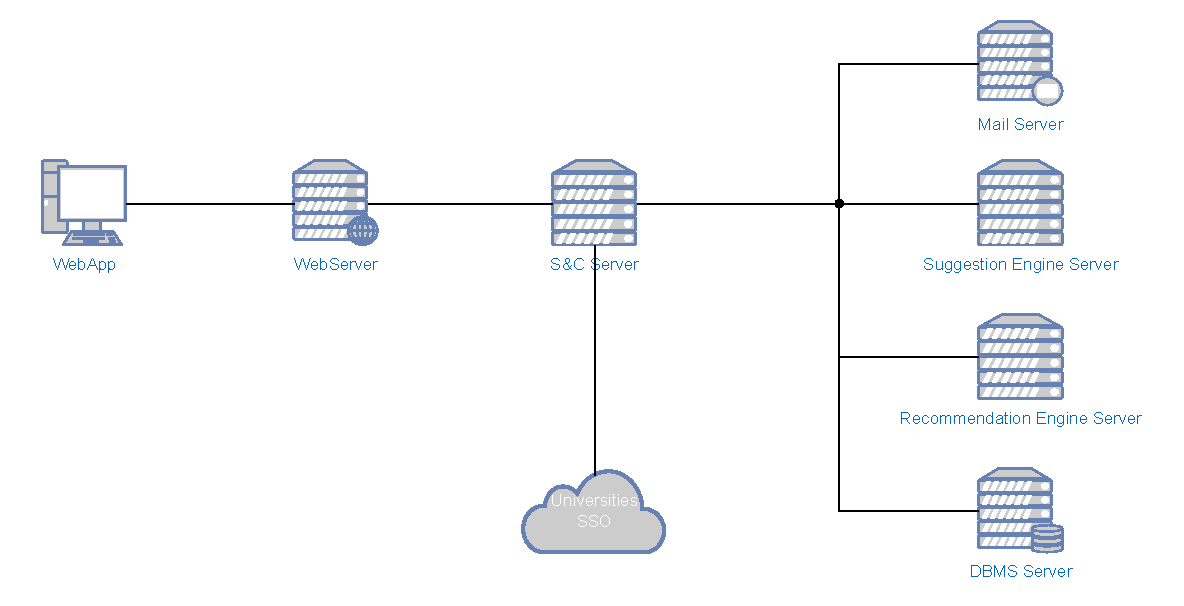
\includegraphics[width=1.0\textwidth]{Images/Overview_diagram.pdf}
    \caption{S\&C Architecture Overview}
    \label{fig:overview}
\end{figure}

\par On the client side, we can see:

\begin{itemize}
    \item \textbf{WebApp}: The web application that the user interacts with, allowing users to connect to S\&C.
                           It is responsible for the user interface and for sending the user's requests to the server.
\end{itemize}

\par On the server side, we can see:

\begin{itemize}
    \item \textbf{Web Server}: It handles communication between users and the S\&C system. It is responsible for
                                receiving the user's requests and distributing them to the different replicas of the S\&C server,
                                performing load balancing. It is also responsible for managing user sessions.
                                It contains the data necessary for students to use university SSOs to log in.

    \item \textbf{S\&C Server}: The main server of the S\&C system. It is the core component of the system and is responsible
                                for communication between the Web Server and the databases and the APIs/Services.
                                It is replicated across multiple machines to ensure high availability and fault tolerance.

    \item \textbf{DBMS Server}: This server archives all the essential information of the system.
                                It stores data related to Users, CVs, Internship Advertisements, and Complaints.
    
    \item \textbf{Recommendation Engine Server}: This server is responsible for generating and searching recommended Internship Advertisements for students and anonymous CVs for companies.
                                                It runs on the same hardware machine as the Suggestions Engine Server using a Docker container.

    \item \textbf{Suggestions Engine Server}: This server is responsible for generating suggestions for improving students' CVs and companies' internship advertisements.
                                            It runs on the same hardware machine as the Recommendation Engine Server using a Docker container.

    \item \textbf{Mail Server}: This server is responsible for sending emails to users. It is used for sending notifications and confirmations of actions performed by users.

\end{itemize}                                

\section{Component View}
\label{sub:component-view}

\subsection{High-Level Components}
\label{sub:high-level-components}

\begin{figure}[H]
    \centering
    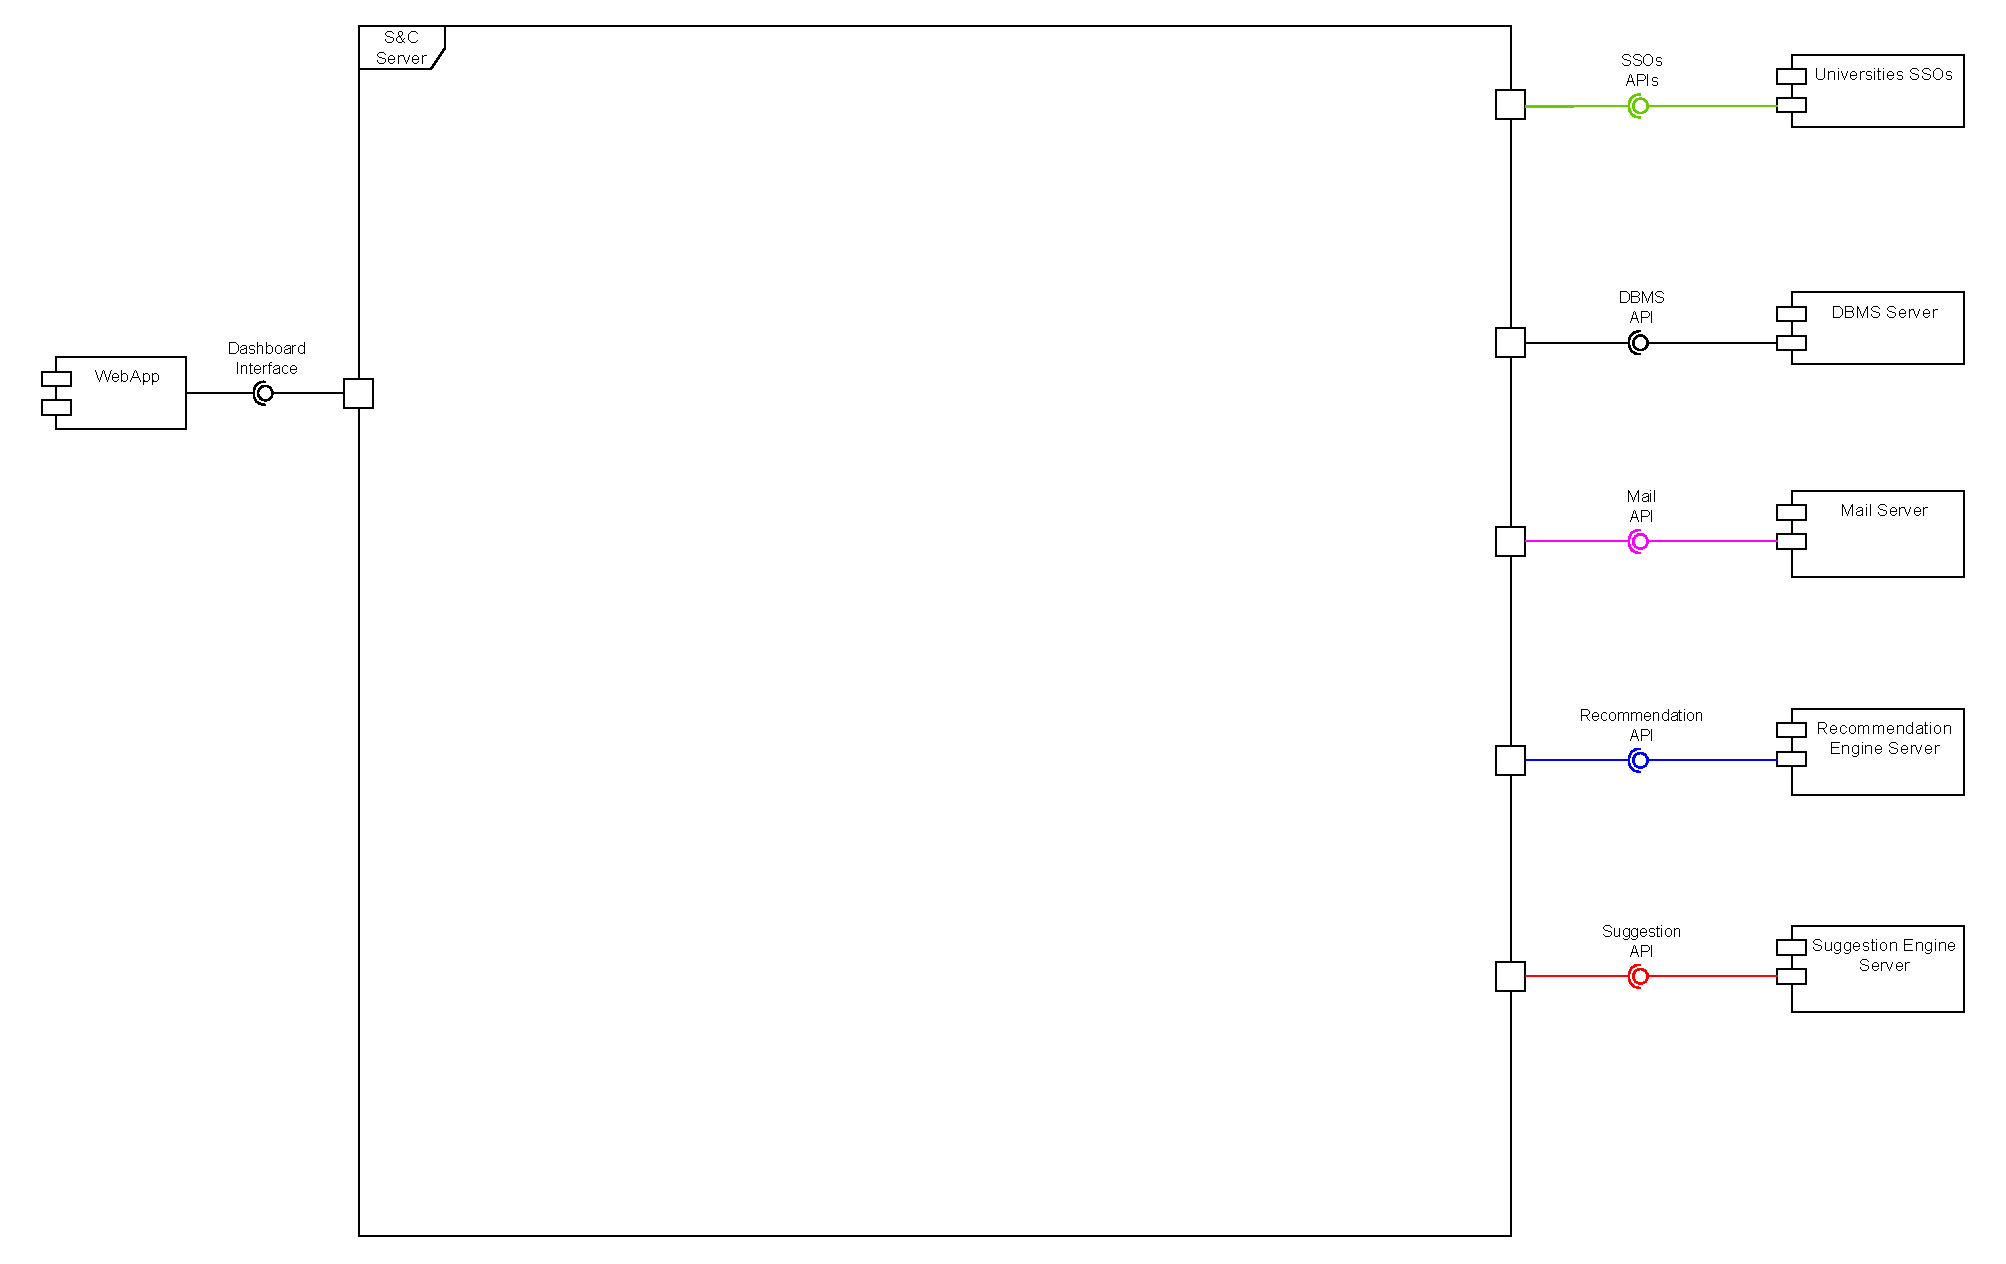
\includegraphics[width=0.8\textwidth]{Images/High_Level_Architectural_Design.pdf}
    \caption{High-Level Components}
    \label{fig:high-level-components}
\end{figure}

\par Figure \ref{fig:high-level-components} shows the high-level components of the S\&C system. The main external components are:

\begin{itemize}
    \item \textbf{WebApp}: This is the web application that the user interacts with. It allows users to communicate 
                            with the S\&C Server through the Dashboard Interface, which is the only means of interaction 
                            between the users and the system. The Dashboard Interface includes multiple functionalities,
                            one of which allows the Dashboard to send notifications to users while they are using the system.
    \item \textbf{DBMS Server}: This server stores all the information of the Users, including their profile information, CVs, 
                                Internship Advertisements, Questionnaires, and Complaints. It is the main component of the system and is 
                                responsible for data management.
    \item \textbf{Mail Server}: This server is responsible for notifying users outside of the web application. 
                                It is used to send all types of notifications, including those confirming actions performed by a user,
                                notifications of new recommendations for both students and companies, requests to fill out questionnaires,
                                and notifications about the creation of new complaints, etc.
    \item \textbf{Recommendation Engine Server}: This server is responsible for generating recommended Internship Advertisements for students 
                                                and anonymous CVs for companies. It periodically retrieves CV data and Internship Advertisement data 
                                                to improve the program responsible for creating suggestions for each user.
    \item \textbf{Suggestions Engine Server}: This server is responsible for generating suggestions for improving students' CVs and companies' internship advertisements.
                                            It periodically retrieves CV data, Internship Advertisement data, and feedback answers at the end of internships 
                                            to improve the program responsible for creating suggestions for each user.
    \item \textbf{Universities SSOs}: This external component allows students to log in to the system using their university credentials.
\end{itemize}


\subsection{Low-Level Components}
\label{sub:low-level-components}

\begin{figure}[H]
    \centering
    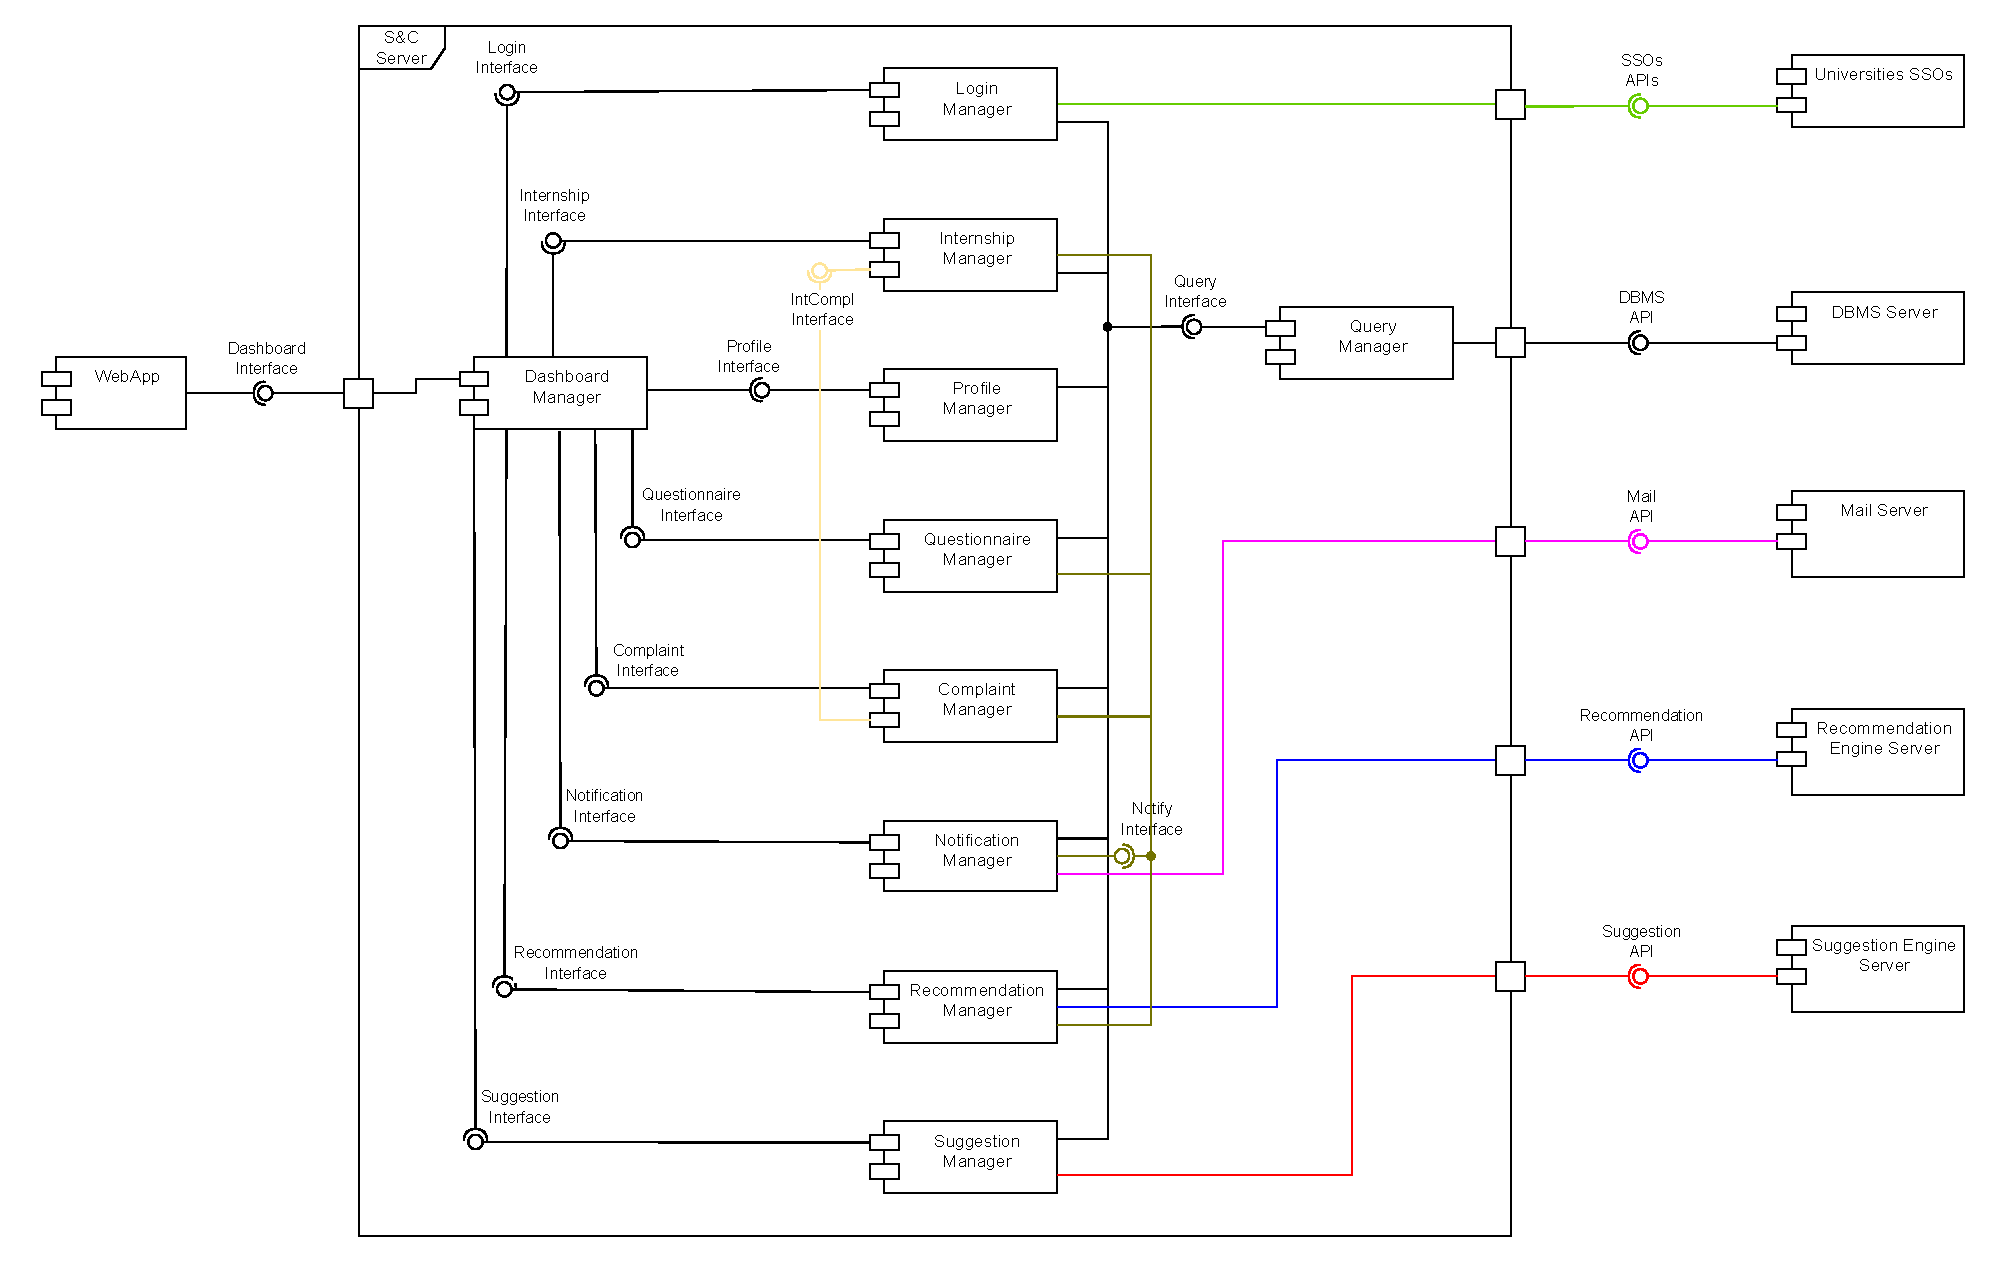
\includegraphics[width=1.0\textwidth]{Images/Low_Level_Architectural_Design.pdf}
    \caption{Low-Level Components}
    \label{fig:low-level-components}
\end{figure}

\par Figure \ref{fig:low-level-components} shows the complete architecture of the S\&C system, detailing the components inside the S\&C Server:

\begin{itemize}
    \item \textbf{Dashboard Manager}: This component is responsible for interacting with users through the dashboard interface.
                                    The Dashboard Manager executes user requests and interacts with the appropriate components.

    \item \textbf{Login Manager}: This component is responsible for user login. For companies and universities,
                                it checks credentials against those stored in the DBMS. For students, it handles the first login (registration) 
                                and subsequent logins by interacting with the Universities SSOs.

    \item \textbf{Internship Manager}: This component manages all stages of the Internship selection and execution process.
                                    It handles the creation of Internship Advertisements, the list of student applications,
                                    and the status of internships. It also provides an interface for the Complaint Manager to modify the status of internships.
    
    \item \textbf{Profile Manager}: This component manages user profiles. It allows users to modify their profile information,
                                    students to upload their CVs, and companies to create their profile descriptions.
    
    \item \textbf{Questionnaire Manager}: This component manages Questionnaires, both those created by companies for selecting students for internships 
    and those created by the system for feedback at the end of internships. 
    
    \item \textbf{Complaints Manager}: This component manages complaints. It is used to create complaints, manage them, and if necessary,
    interact with the related internship to modify its status through the interface provided by the Internship Manager.
    
    \item \textbf{Notification Manager}: This component manages notifications. It generates notifications to send to the 
    dashboard if the user is logged in, and interacts with the Mail Server to send notifications to users outside of the web application.
    
    \item \textbf{Recommendation Manager}: This component interacts with the Recommendation Engine Server. It retrieves the data
    required by the recommendation engine to improve its suggestions, and retrieves the results of the recommendation engine to display to users. 
    
    \item \textbf{Suggestions Manager}: This component interacts with the Suggestions Engine Server. It retrieves the data
    required by the suggestion engine to improve its suggestions, and retrieves the results of the suggestion engine to display to users.
    
    \item \textbf{Query Manager}: This component executes queries and converts the data returned by the DBMS into the necessary objects for other components.
\end{itemize}

\subsubsection{Login Manager}
\label{subsub:login-manager}

\begin{figure}[H]
      \centering
      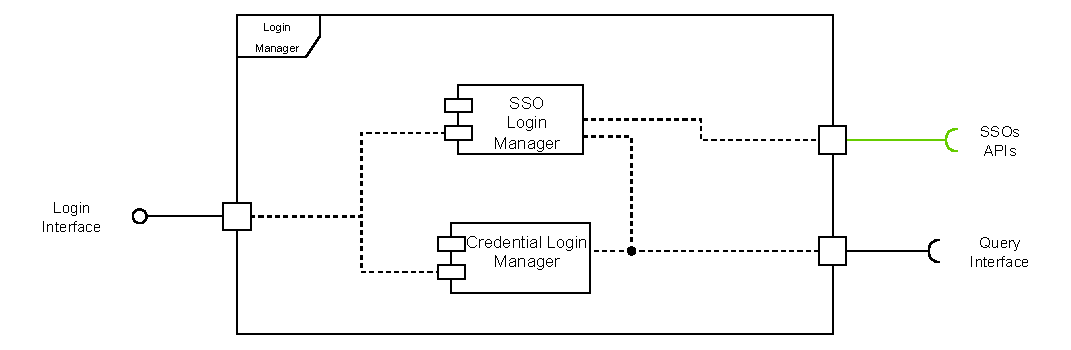
\includegraphics[width=0.8\textwidth]{Images/Login_Architecture.pdf}
      \caption{Login Manager}
      \label{login-manager-arch}
\end{figure}

\par The Login Manager is composed of other two sub-components:
\begin{itemize}
      \item \textbf{Student Login Manager}: This component is responsible for managing student logins
            and their registration. It interacts with the Universities SSOs to authenticate students.
      \item \textbf{COUN Login Manager}: This component is responsible for managing company and university logins.
            It checks the credentials against those stored in the DBMS.
\end{itemize}

\subsubsection{Profile Manager}
\label{subsub:profile-manager}

\begin{figure}[H]
      \centering
      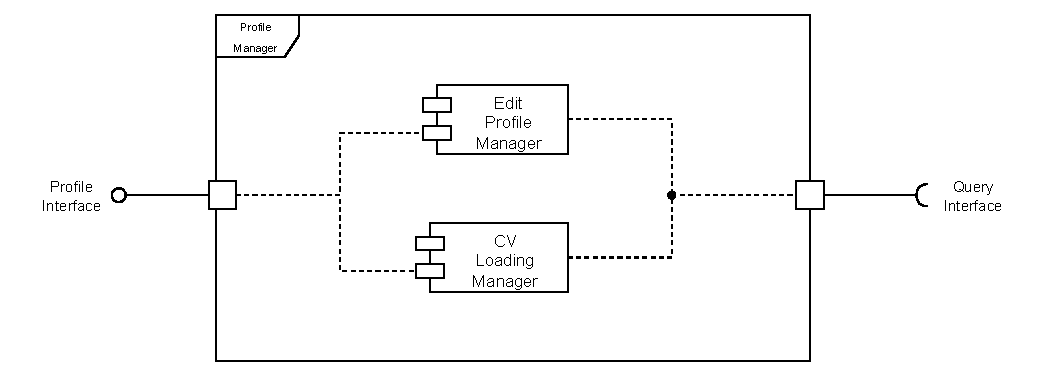
\includegraphics[width=0.8\textwidth]{Images/Profile_Architecture.pdf}
      \caption{Profile Manager}
      \label{profile-manager-arch}
\end{figure}

\par The Profile Manager is composed of other two sub-components:
\begin{itemize}
      \item \textbf{Profile Manager}: This component is responsible for the modification of the user's profile information.
            For the compnaies it allows to create their profile description that will be shown to students.
      \item \textbf{CV Manager}: This component is responsible for the management of the student's CVs and uploading them.
\end{itemize}

\subsubsection{Questionnaire Manager}
\label{subsub:questionnaire-manager}

\begin{figure}[H]
      \centering
      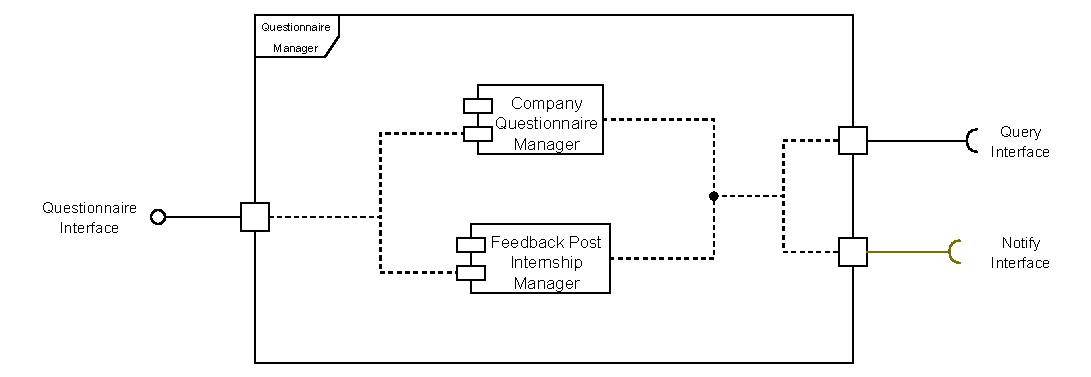
\includegraphics[width=0.8\textwidth]{Images/Questionnaire_Architecture.pdf}
      \caption{Profile Manager}
      \label{questionnaire-manager-arch}
\end{figure}

\par The Questionnaire Manager is composed of other two sub-components:
\begin{itemize}
      \item \textbf{Company Questionnaire Manager}: This component is responsible for managing the questionnaires created by companies.
            It allows companies to create, modify and delate questionnaires to select students for internships.
            It allows commpanies to see the answers to the questionnaires.
      \item \textbf{Feedback Questionnaire Manager}: This component is responsible for managing the feedback questionnaires created by the system.
            It allows the system to create questionnaires for feedback at the end of internships.
\end{itemize}

\section{Deployment View}

\begin{figure}[H]
    \centering
    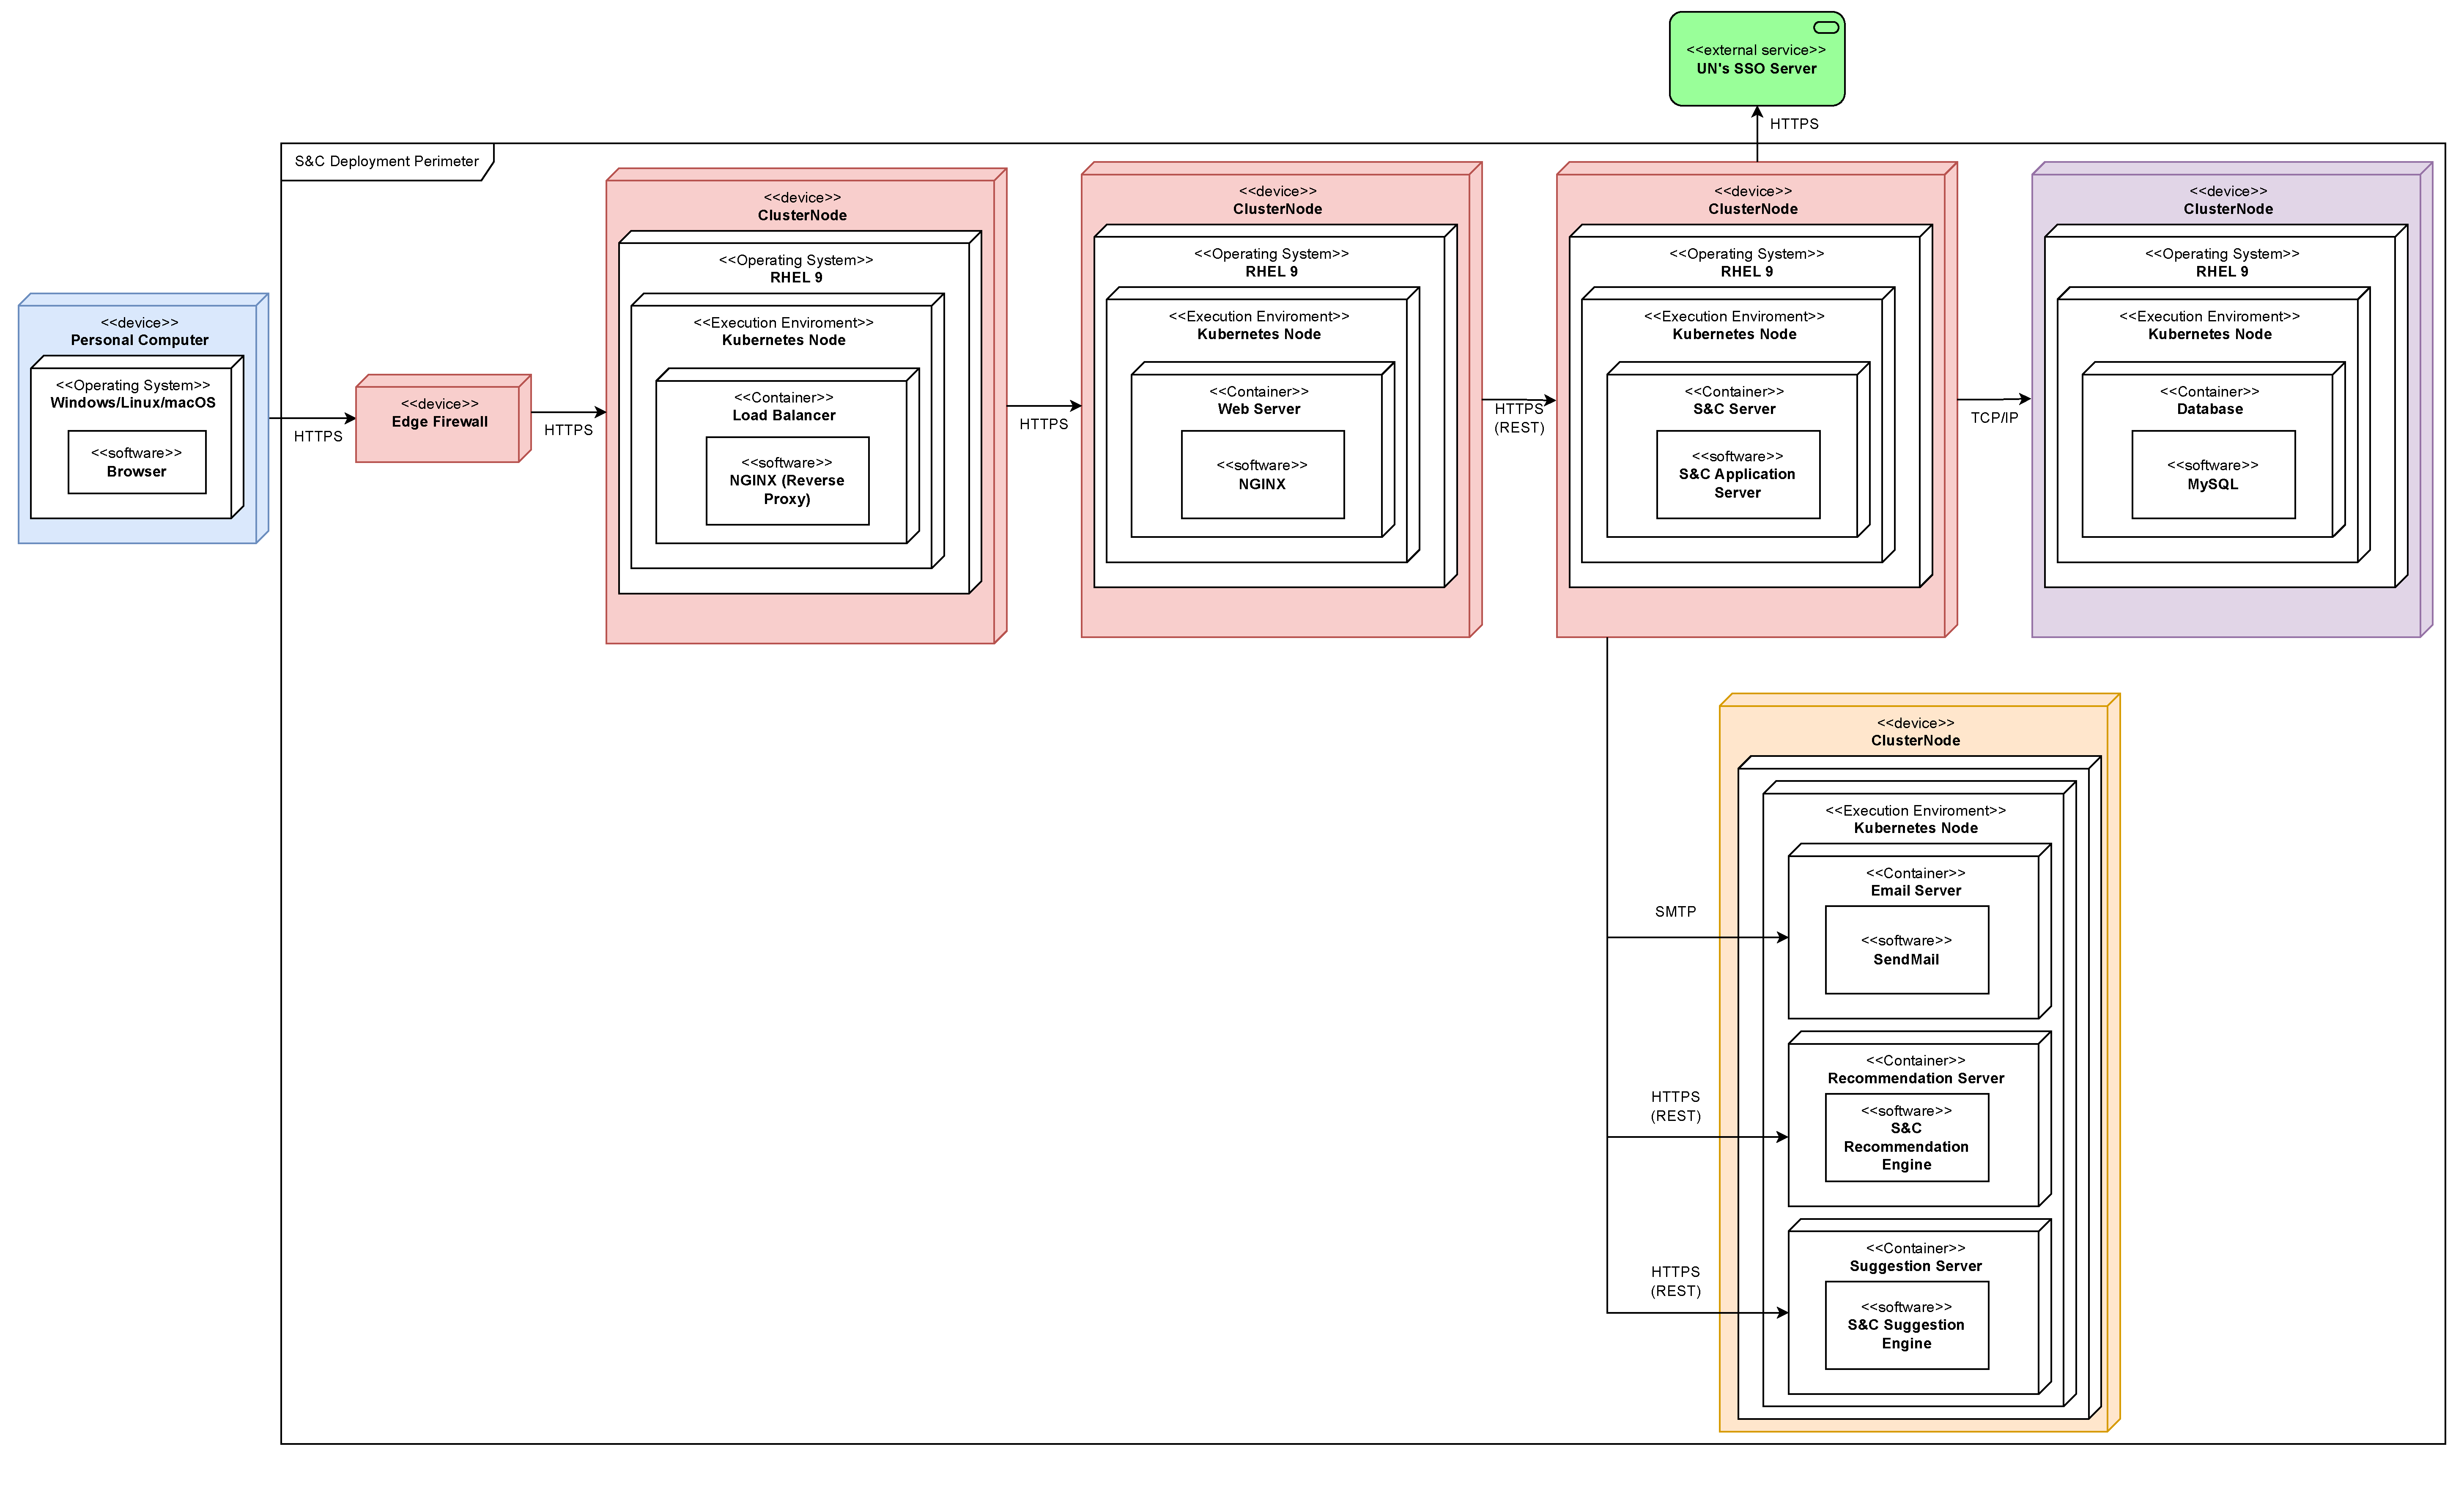
\includegraphics[width=1.0\textwidth]{Images/Deployment_Diagram.pdf}
    \caption{Deployment Diagram}
    \label{fig:deployment-diagram}
\end{figure}

% This should be section 2.6. of the DD.

\section{Selected Architectural Styles and Patterns}
\label{sec:selected-architectural-styles-patterns}%

\par{\textbf{Architectural Design:}} The architectural design of S\&C is based on the industry-standard 3-Tier-Architecture pattern:

\begin{enumerate}
      \item \textbf{Presentation Tier:} This is the upper layer that directly interacts with users. The presentation tier
            focuses on displaying information to the user and capturing user inputs. It's designed to handle all client-side
            interactions and renders the application's visual components.
      \item \textbf{Application Tier:} This layer contains the core business logic and processing rules of the
            application. It receives requests from the presentation tier, applies business rules, validates data, and
            coordinates the flow of information. This tier acts as an intermediary, ensuring that data is processed
            according to the application's specific requirements before being passed to or retrieved from the data tier.
      \item \textbf{Data Tier:} The bottom layer of the architecture, responsible for storing, retrieving, and managing
            data. The data tier ensures data integrity, provides database connection management, and implements data
            access methods that the application tier can use to interact with the stored information.
\end{enumerate}

The division of the system into these three layers allows a reduction in complexity, improves maintainability, and
facilitates scalability: each layer can be developed, tested, deployed and maintained independently, enabling a more
modular and flexible system architecture while also parallelizing development efforts.

The choice of a 3-Tier-Architecture is also motivated by the fact that it can be easily mapped to the MVC
(Model-View-Controller) pattern - a widely-used design pattern that separates the application into three interconnected
components: the Model (data), the View (interface), and the Controller (business logic). This pattern is particularly
useful since it allows for a clear separation of concerns and a more modular and maintainable codebase.

Each tier will be run inside a container environment (e.g. Docker) to ensure isolation and scalability. The containers
will be orchestrated (using adequate solutions e.g. Kubernetes) which will also manage the deployment and scaling of
the application.

\par{\textbf{Client-Server Communication:}} S\&C - like almost all modern web applications - is based on a
Client-Server architecture. The client (the user's browser) sends requests to the server, which processes them and
returns the appropriate responses. All the static content (HTML, CSS, JavaScript) is served directly using HTTPS, while
the dynamic content is generated by the server and sent back to the client as JSON data (REST over HTTPS) to be
rendered by the client-side JavaScript code.

\par{\textbf{Intra-Server Communication:}} The communication between the presentation tier and the application tier
will be based on gRPC over TCP/IP. gRPC is a high-performance, open-source, universal RPC framework that can run in any
environment allowing for an easy and efficient communication between the two tiers. The communication between the
application tier and the data tier will be based on SQL Queries over TCP/IP (as implemented by the database driver).

\section{Other Design Decisions}
\label{sec:other-design-decisions}%

\par{Helpers:} In \ref{sec:selected-architectural-styles-patterns} we said that the application tier is running inside a
container. While this is true it must be noted that the application is not fully monolithic. The application tier is
composed of:

\begin{itemize}
      \item \textbf{Core:} The core of the application, it contains the business logic and the processing rules. It is
            the part that communicates with the data tier and the presentation tier.
      \item \textbf{Email Service:} A service that sends emails to users. It is a separate service because it is not
            strictly related to the core of the application and it can be easily scaled independently. Communicates
            with the core using SMTP over TCP/IP. Core prepares the email and sends it to the email service which
            sends it to the user.
      \item \textbf{Recommendation Engine:} A service that provides internships recommendations to STs. Communicates
            with the core using gRPC over TCP/IP. Core asks the recommendation engine for recommendations and the
            recommendation engine provides them.
      \item \textbf{Suggestion Engine:} A service that proposes STs to COs (as described in the RASD). Communicates with
            the core using gRPC over TCP/IP like the recommendation engine.
\end{itemize}

It should be also remarked that the application tier communicates with (external to S\&C) the various UN's SSOs using
HTTPS.

\par{\textbf{Networking:}} The internal S\&C network will solely rely on IPv6. This choice is motivated by the fact that
IPv6 is cheaper to maintain, more secure, and more scalable than IPv4. The load balancer at the edge will provide IPv4
connectivity to the outside world for compatibility reasons but all internal communication will be done using IPv6.
This choice will also make easier a multi-cloud deployment in the future.


\chapter{User Interface Design}
\label{chap:user-interface-design}%

\par This section aims to provide a overview of the UI/UX of S\&C. The main focus will be on describing the rationale
that led to the design choices of the UI and the UX instead of providing a detailed description of all the UI
components: the interface should be intuitive and easy to use and, as such, the design should be self-explanatory.

\par The interface will be presented in a series of mockups that will follow the user flow of the application. Each
user type will have its own flow and, as such, its own section. For the sake of clarity, some trivial mockups -
especially if already presented in one of the previous sections - will be omitted in favor of more complex ones; a
short description of the omitted mockups will be provided for consistency.

\par Even if the interface is fully responsive, the mockups will be presented in a desktop format for better
readability. The mobile version will have the same structure and the same components, but will be optimized for
smaller screens.

\section{User Flow: ST}
\label{sec:user-flow-st}%

\begin{figure}[H]
    \centering
    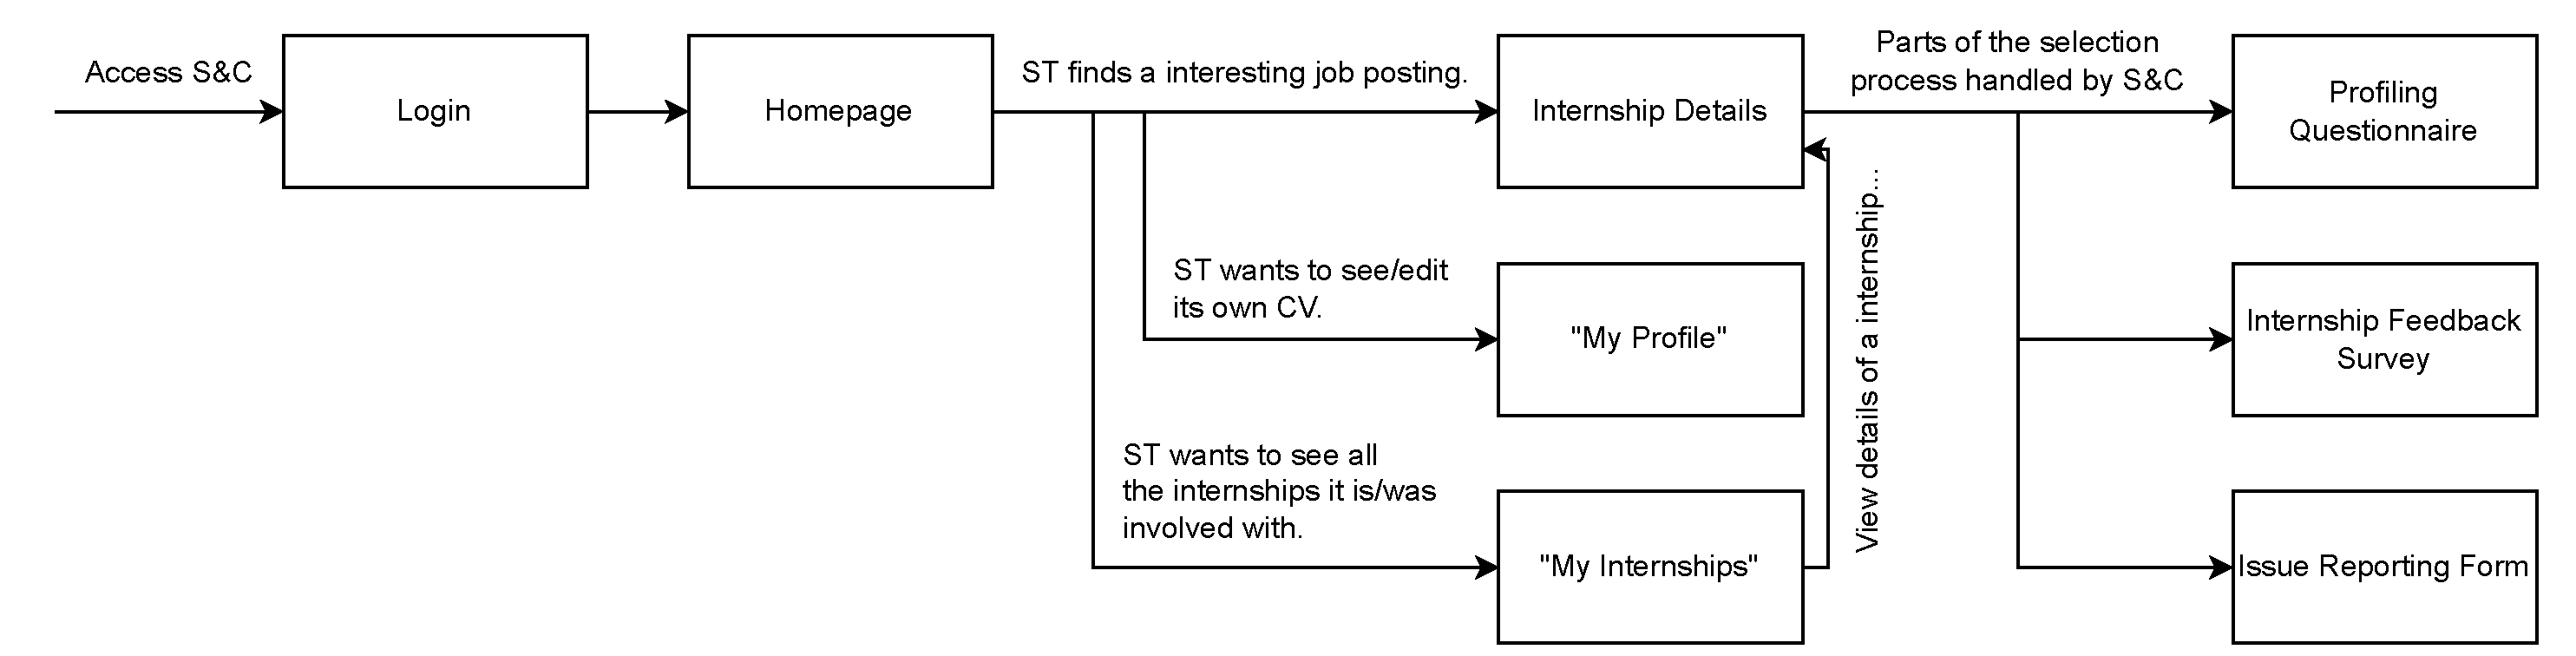
\includegraphics[width=1.0\textwidth]{Images/GUI/ST/Diagram.pdf}
    \caption{ST User Flow Diagram}
    \label{fig:st-user-flow-diagram}
\end{figure}

\par Here is presented the user flow diagram for the ST. The ST uses the Login page to authenticate and access S\&C
and then is redirected to the Homepage. Here the user can discover new internships and view their details
(Internship Details). The Internship Details page will allow the user to apply for the internship, access the
Profiling Questionnaire, reports violations using the Issue Reporting Form and, once the internship is over,
access the Internship Feedback Survey. By using the functions in the header the user can access their own profile
("My Profile"), view all the internships they have interacted with ("My Internships") and log out of the system.

\subsection{Login - ST}
\label{subsec:login-st}%

\begin{figure}[H]
    \centering
    \fbox{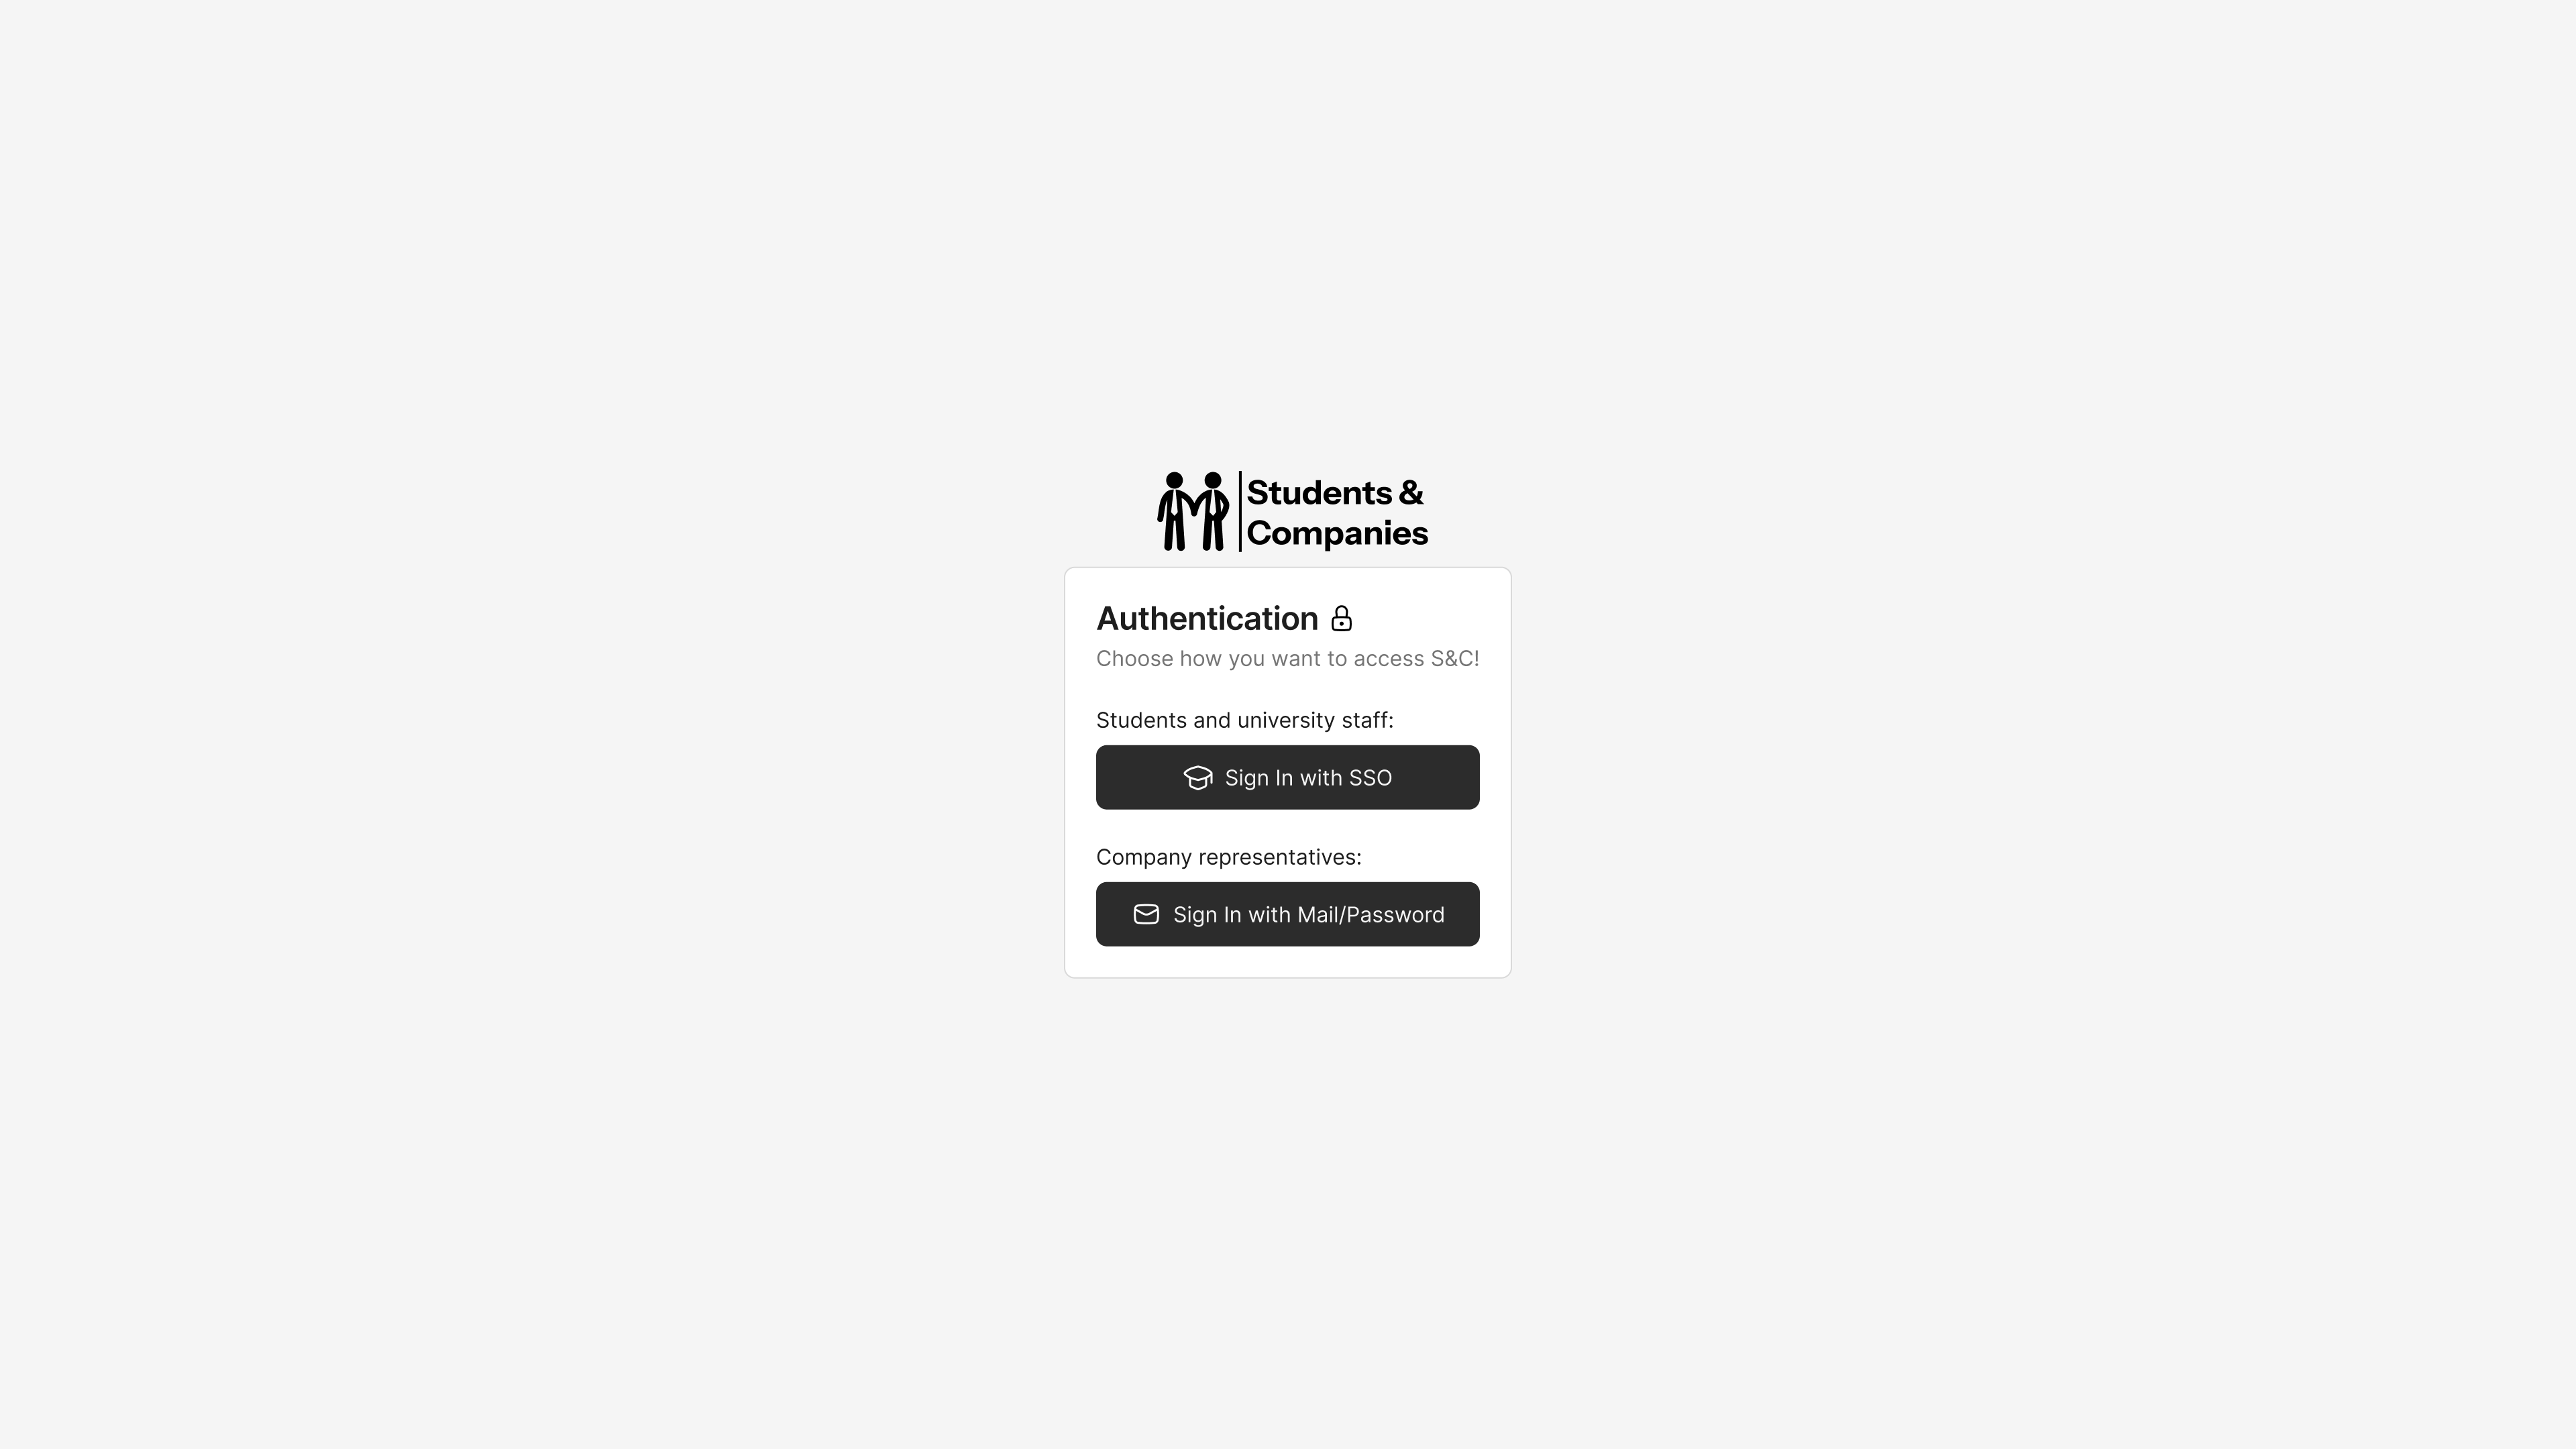
\includegraphics[width=1.0\textwidth]{Images/GUI/ST/Login - ST.png}}
    \caption{Login Page - ST}
    \label{fig:login-page-st}
\end{figure}

\par The login page is the first page the ST will see when accessing the S\&C platform. While ST and UN will use their
university authentication service to log in, a button to use standard credentials is also provided for CO users.

\subsection{Homepage - ST}
\label{subsec:homepage-st}%

\begin{figure}[H]
    \centering
    \fbox{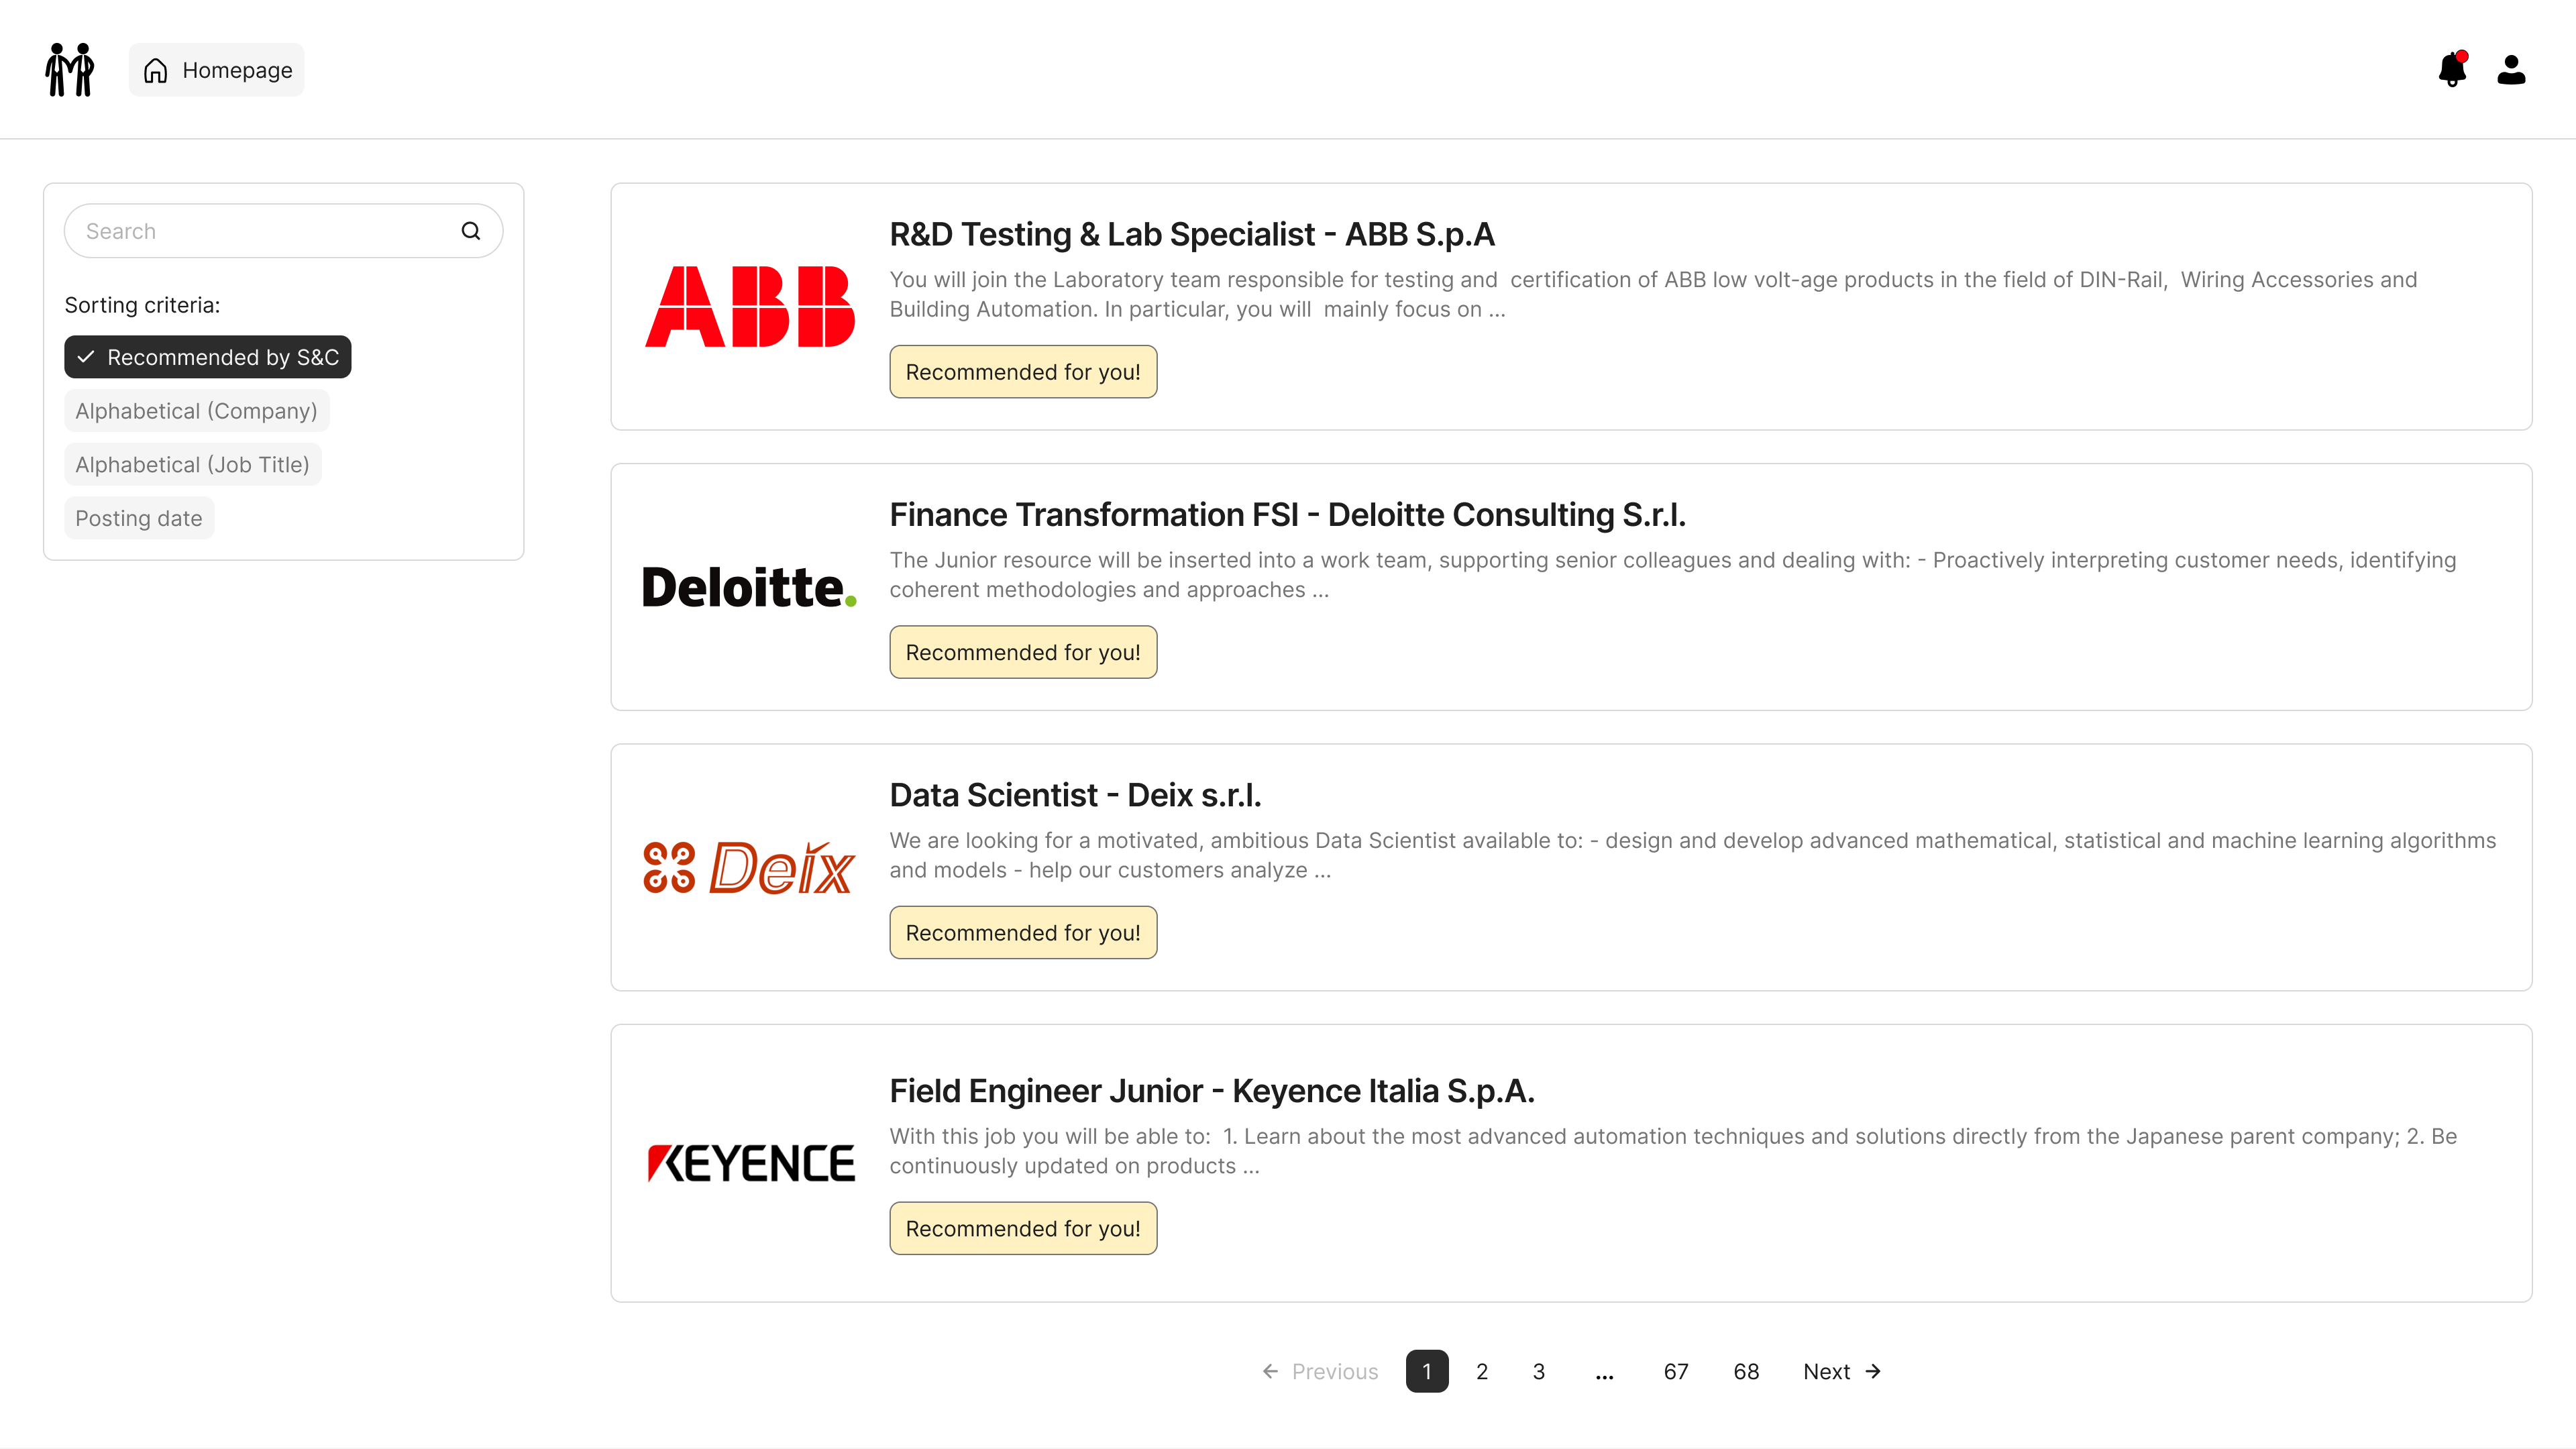
\includegraphics[width=1.0\textwidth]{Images/GUI/ST/Homepage - ST.png}}
    \caption{Homepage - ST}
    \label{fig:homepage-st}
\end{figure}

\par The homepage is the main page for the ST. Here the user can discover new internships and view their details. As
all the other pages, the header is present and allows the user to access their profile, view their internships and
log out. Also, a notification submenu is present to show the user any new notifications in case they missed the email.

\par Appropriate filters are provided to allow the user to search for internships based on their preferences.

\begin{figure}[H]
    \centering
    \fbox{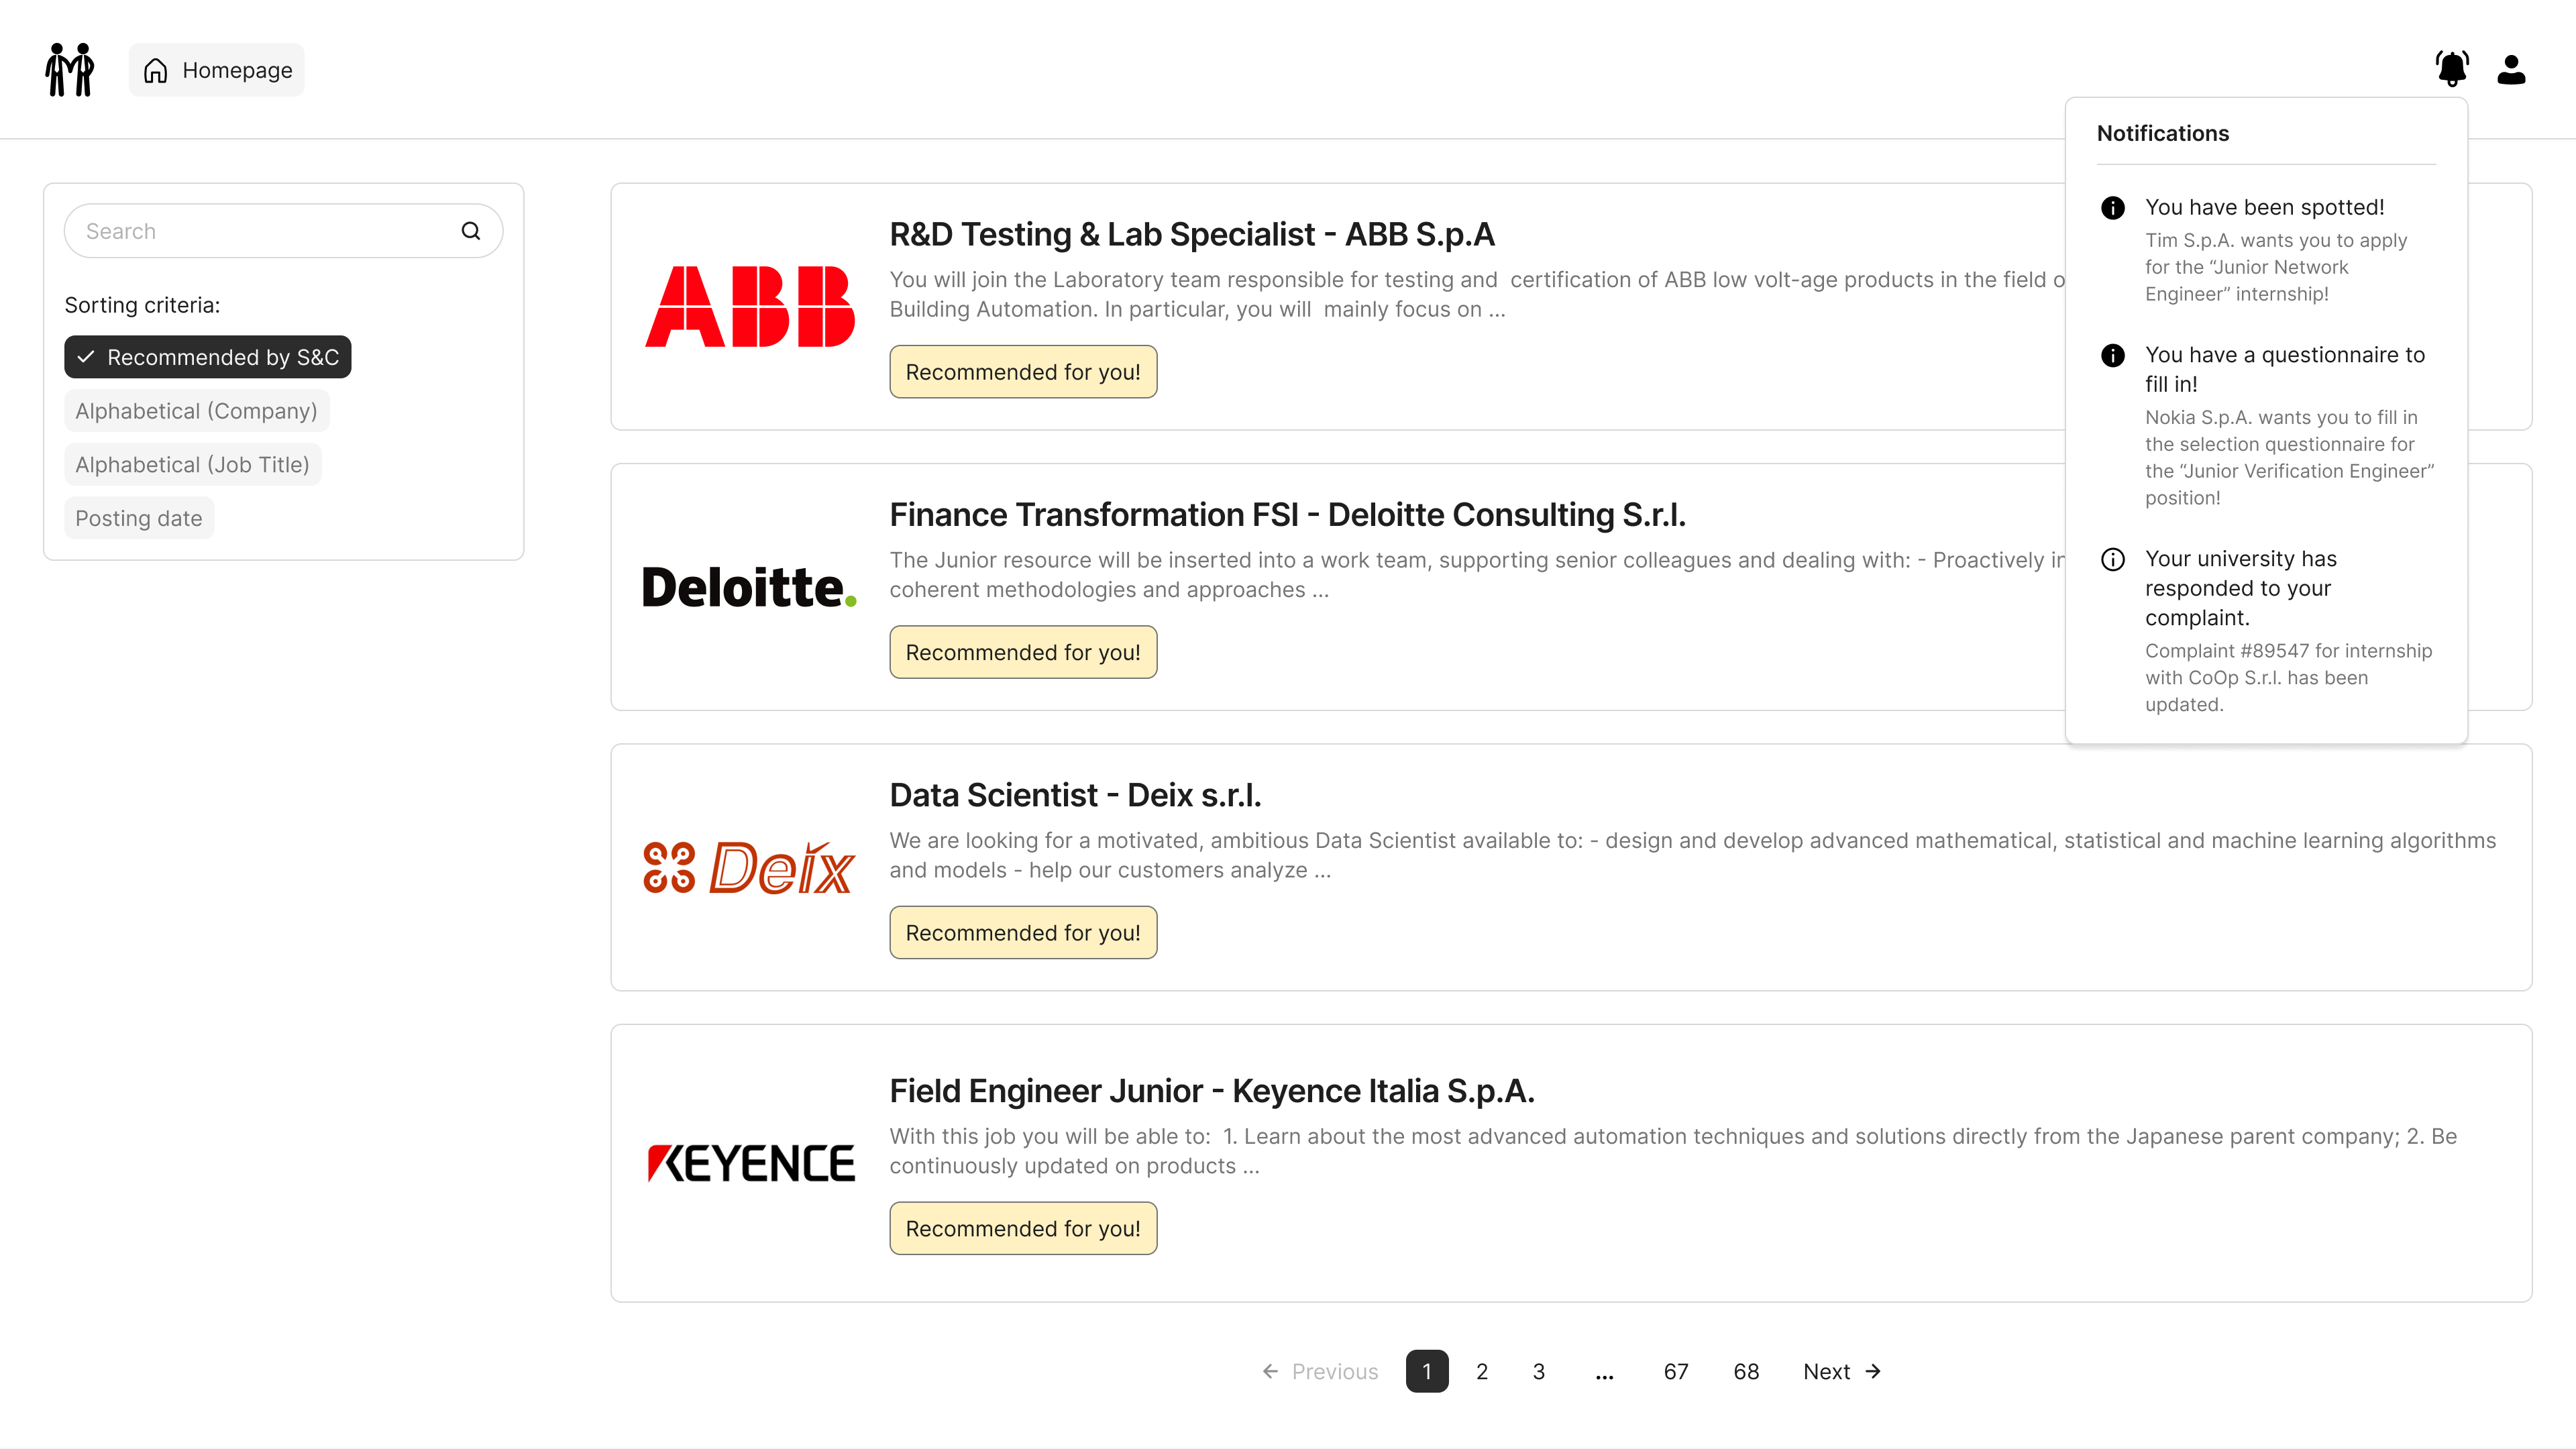
\includegraphics[width=1.0\textwidth]{Images/GUI/ST/Homepage - ST - Notification.png}}
    \caption{Homepage - ST - Notification}
    \label{fig:homepage-st-notification}
\end{figure}

\begin{figure}[H]
    \centering
    \fbox{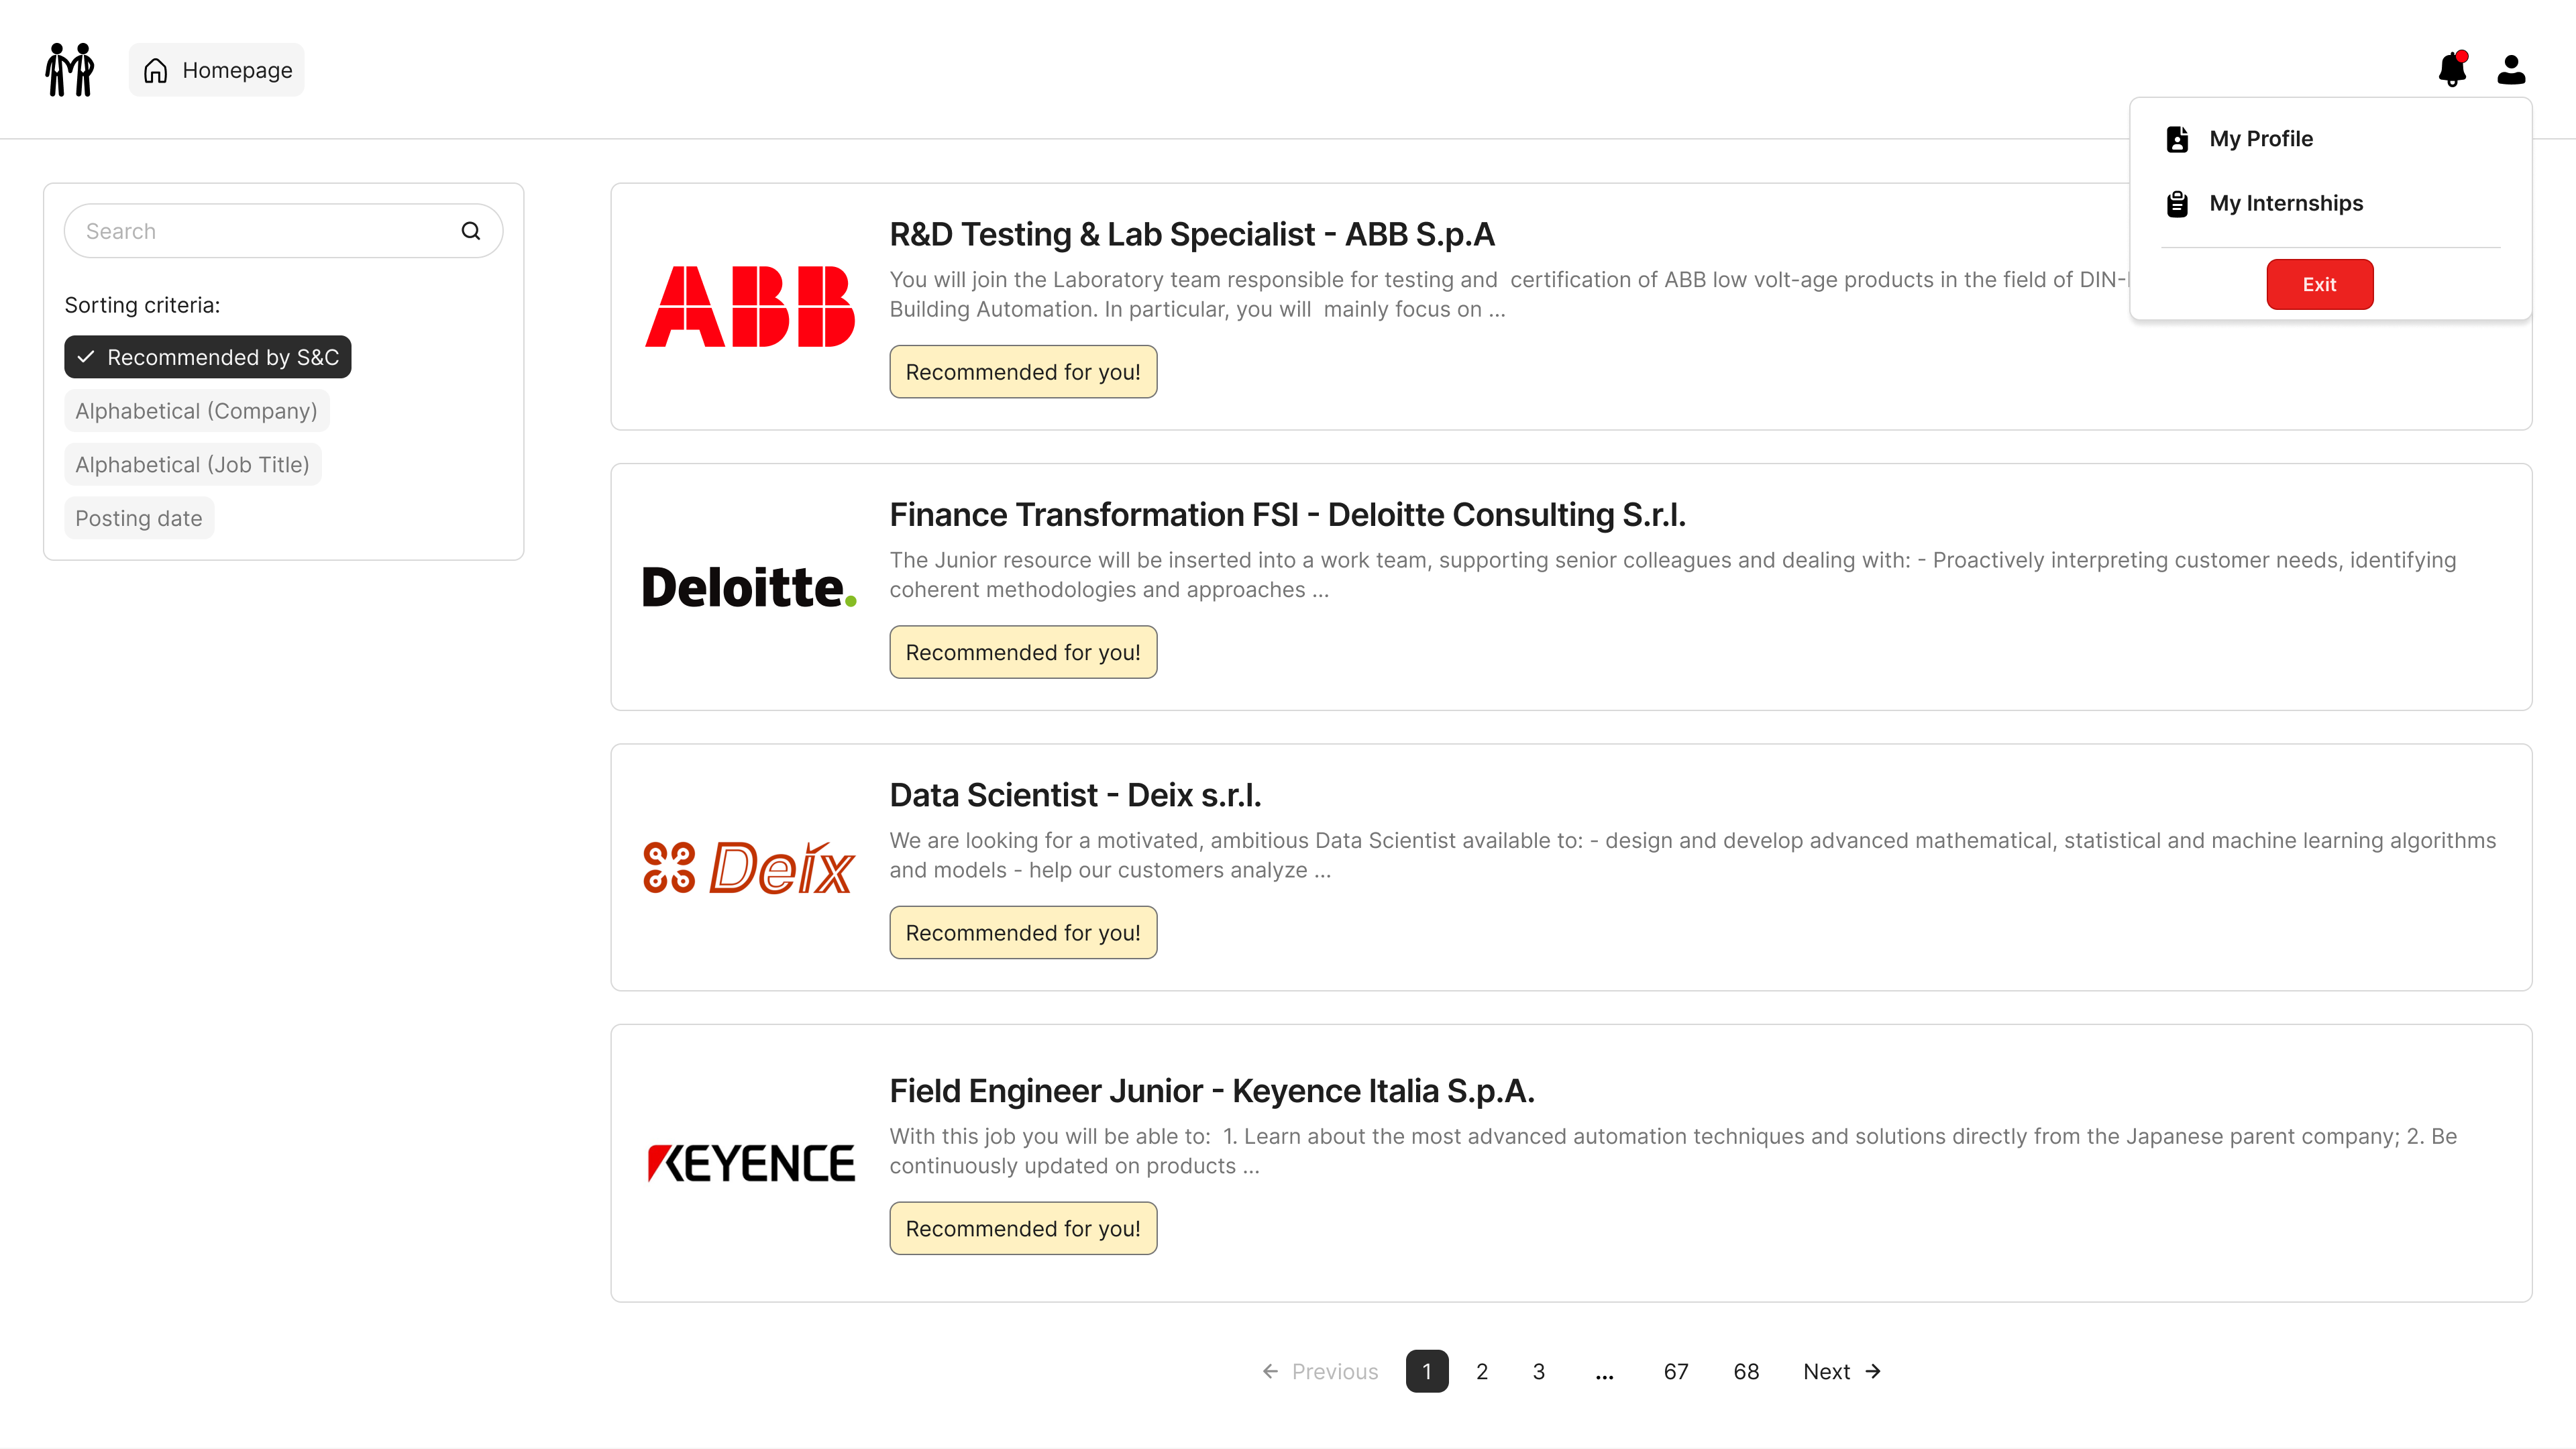
\includegraphics[width=1.0\textwidth]{Images/GUI/ST/Homepage - ST - Profile.png}}
    \caption{Homepage - ST - Profile}
    \label{fig:homepage-st-profile}
\end{figure}

\subsection{"My Internships" - ST}
\label{subsec:my-internships-st}%

\begin{figure}[H]
    \centering
    \fbox{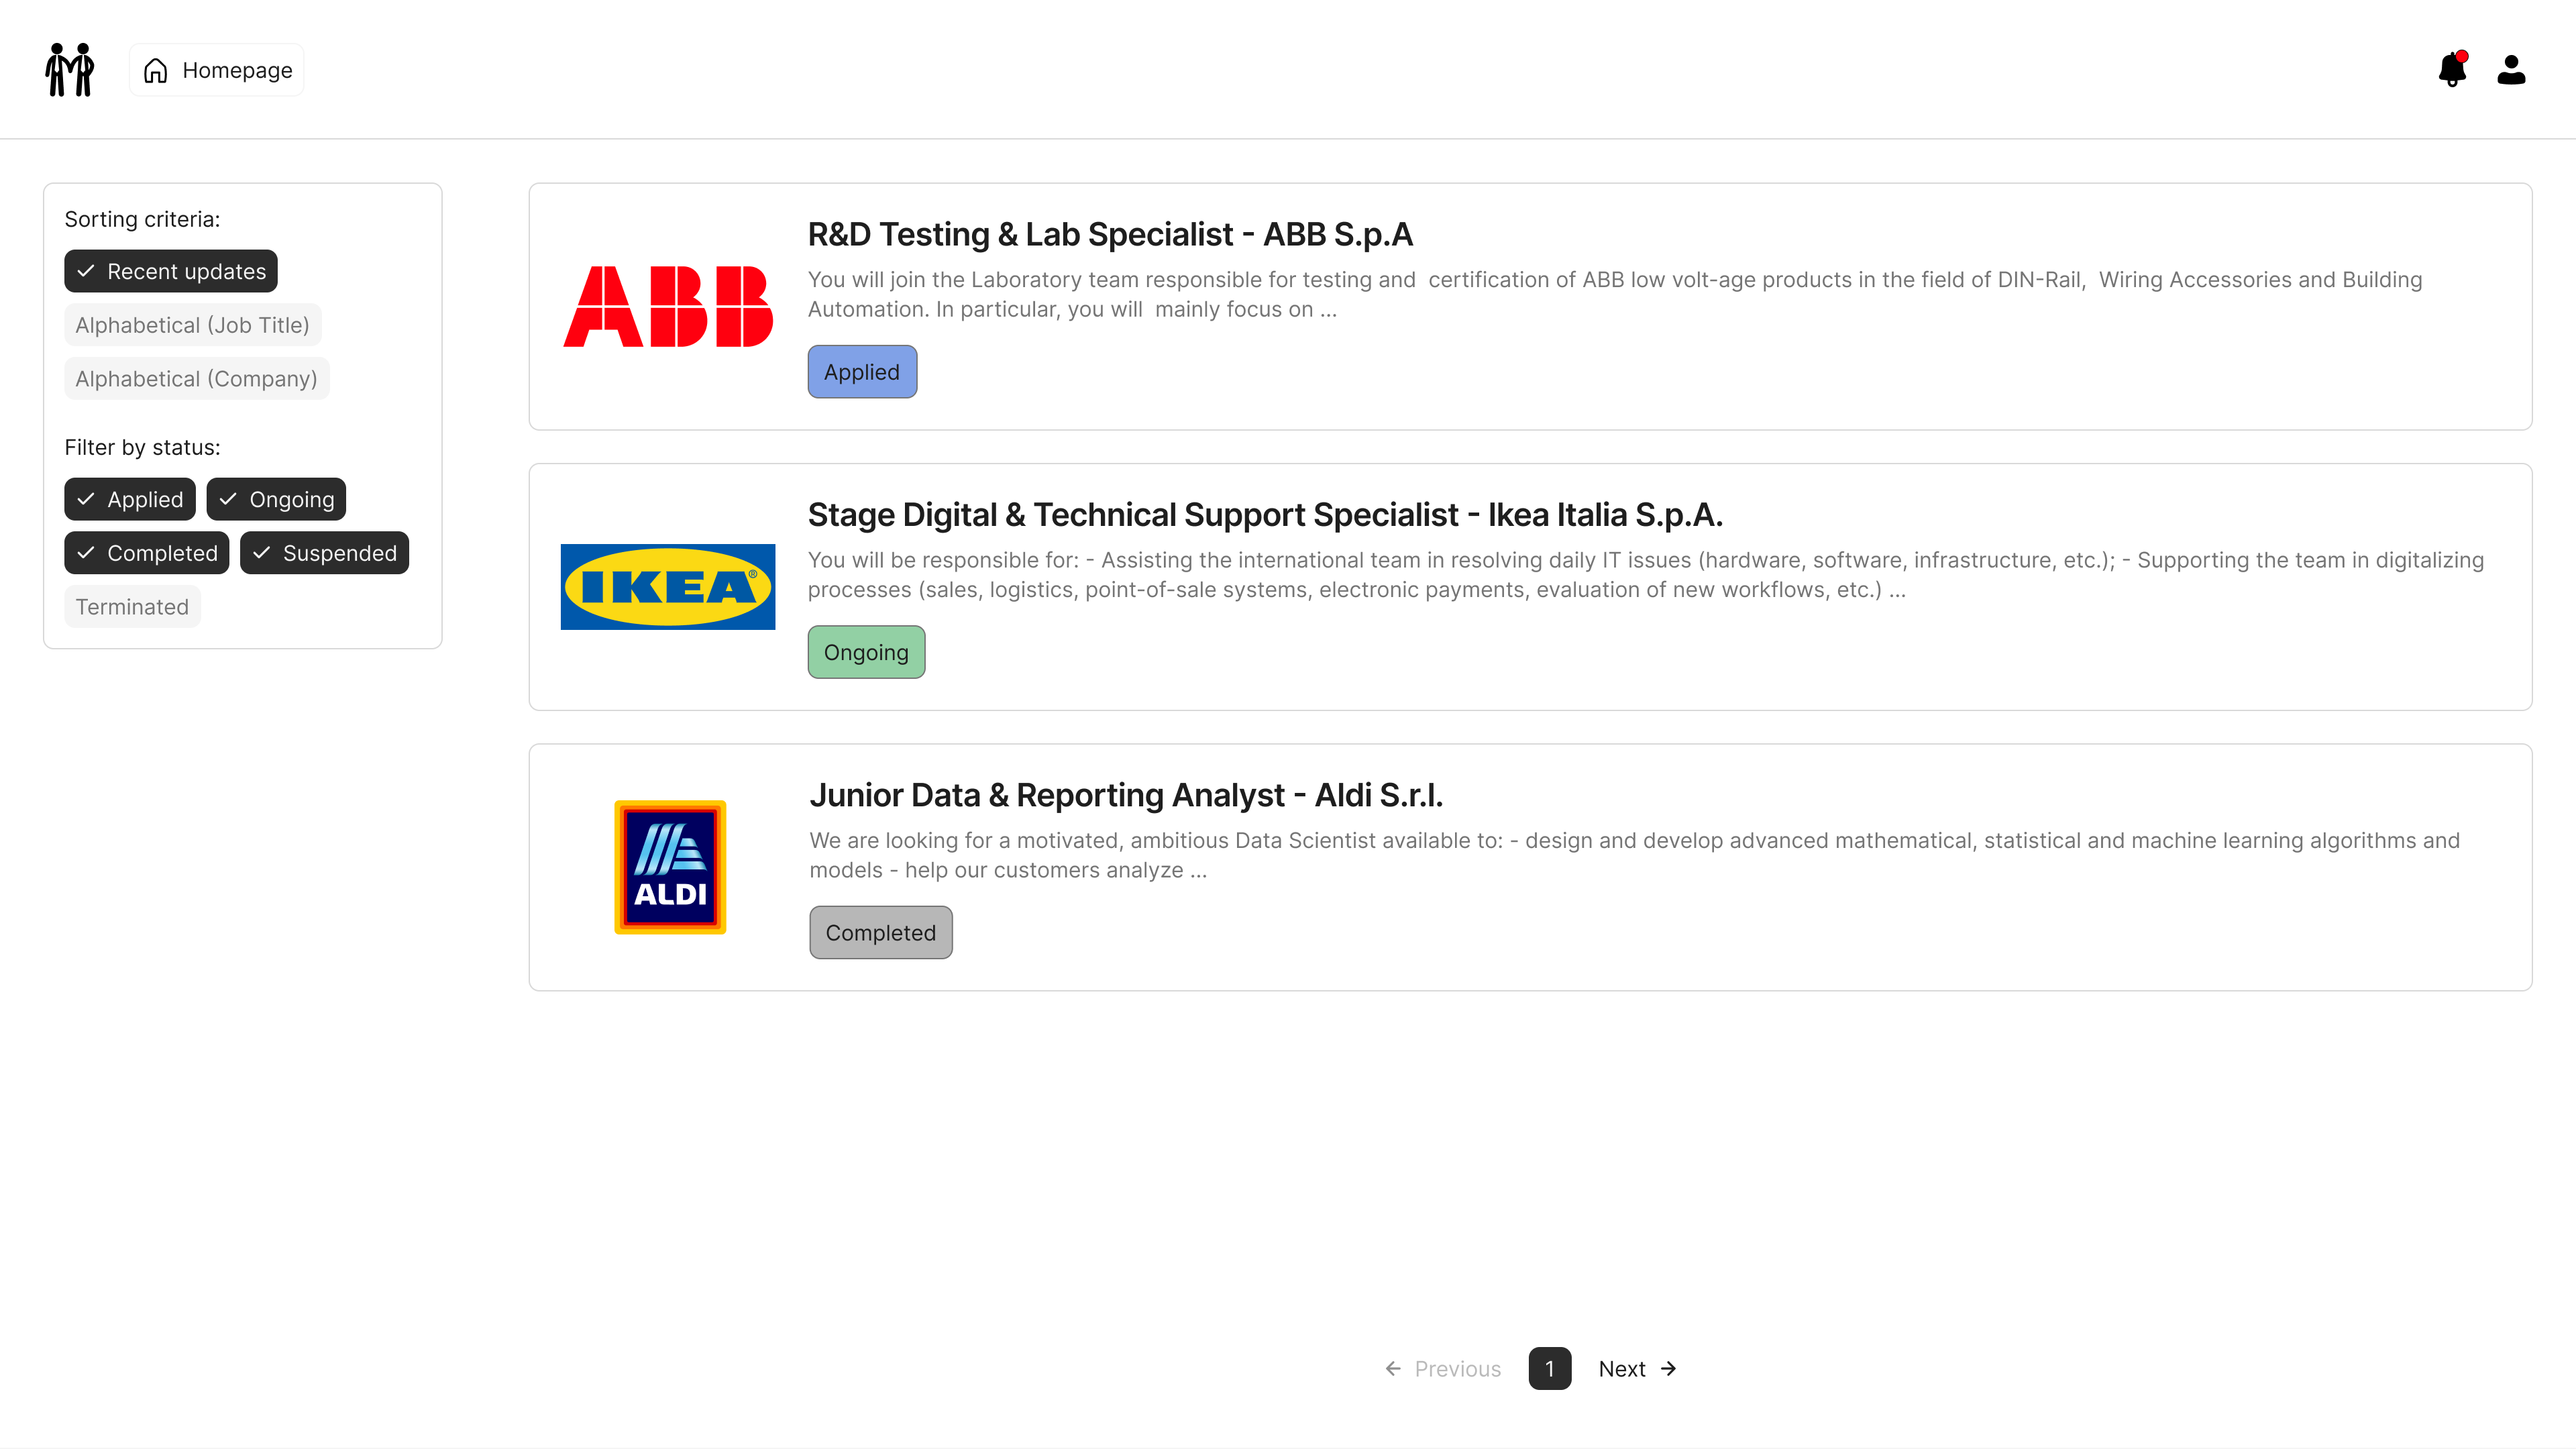
\includegraphics[width=1.0\textwidth]{Images/GUI/ST/My Internships - ST.png}}
    \caption{"My Internships" - ST}
    \label{fig:my-internships-st}
\end{figure}

\par The "My Internships" page allows the ST to view all the internships they have interacted with. It is similar to
the homepage and as such filters are provided.

\subsection{"My Profile" - ST}
\label{subsec:profile-st}%

\begin{figure}[H]
    \centering
    \fbox{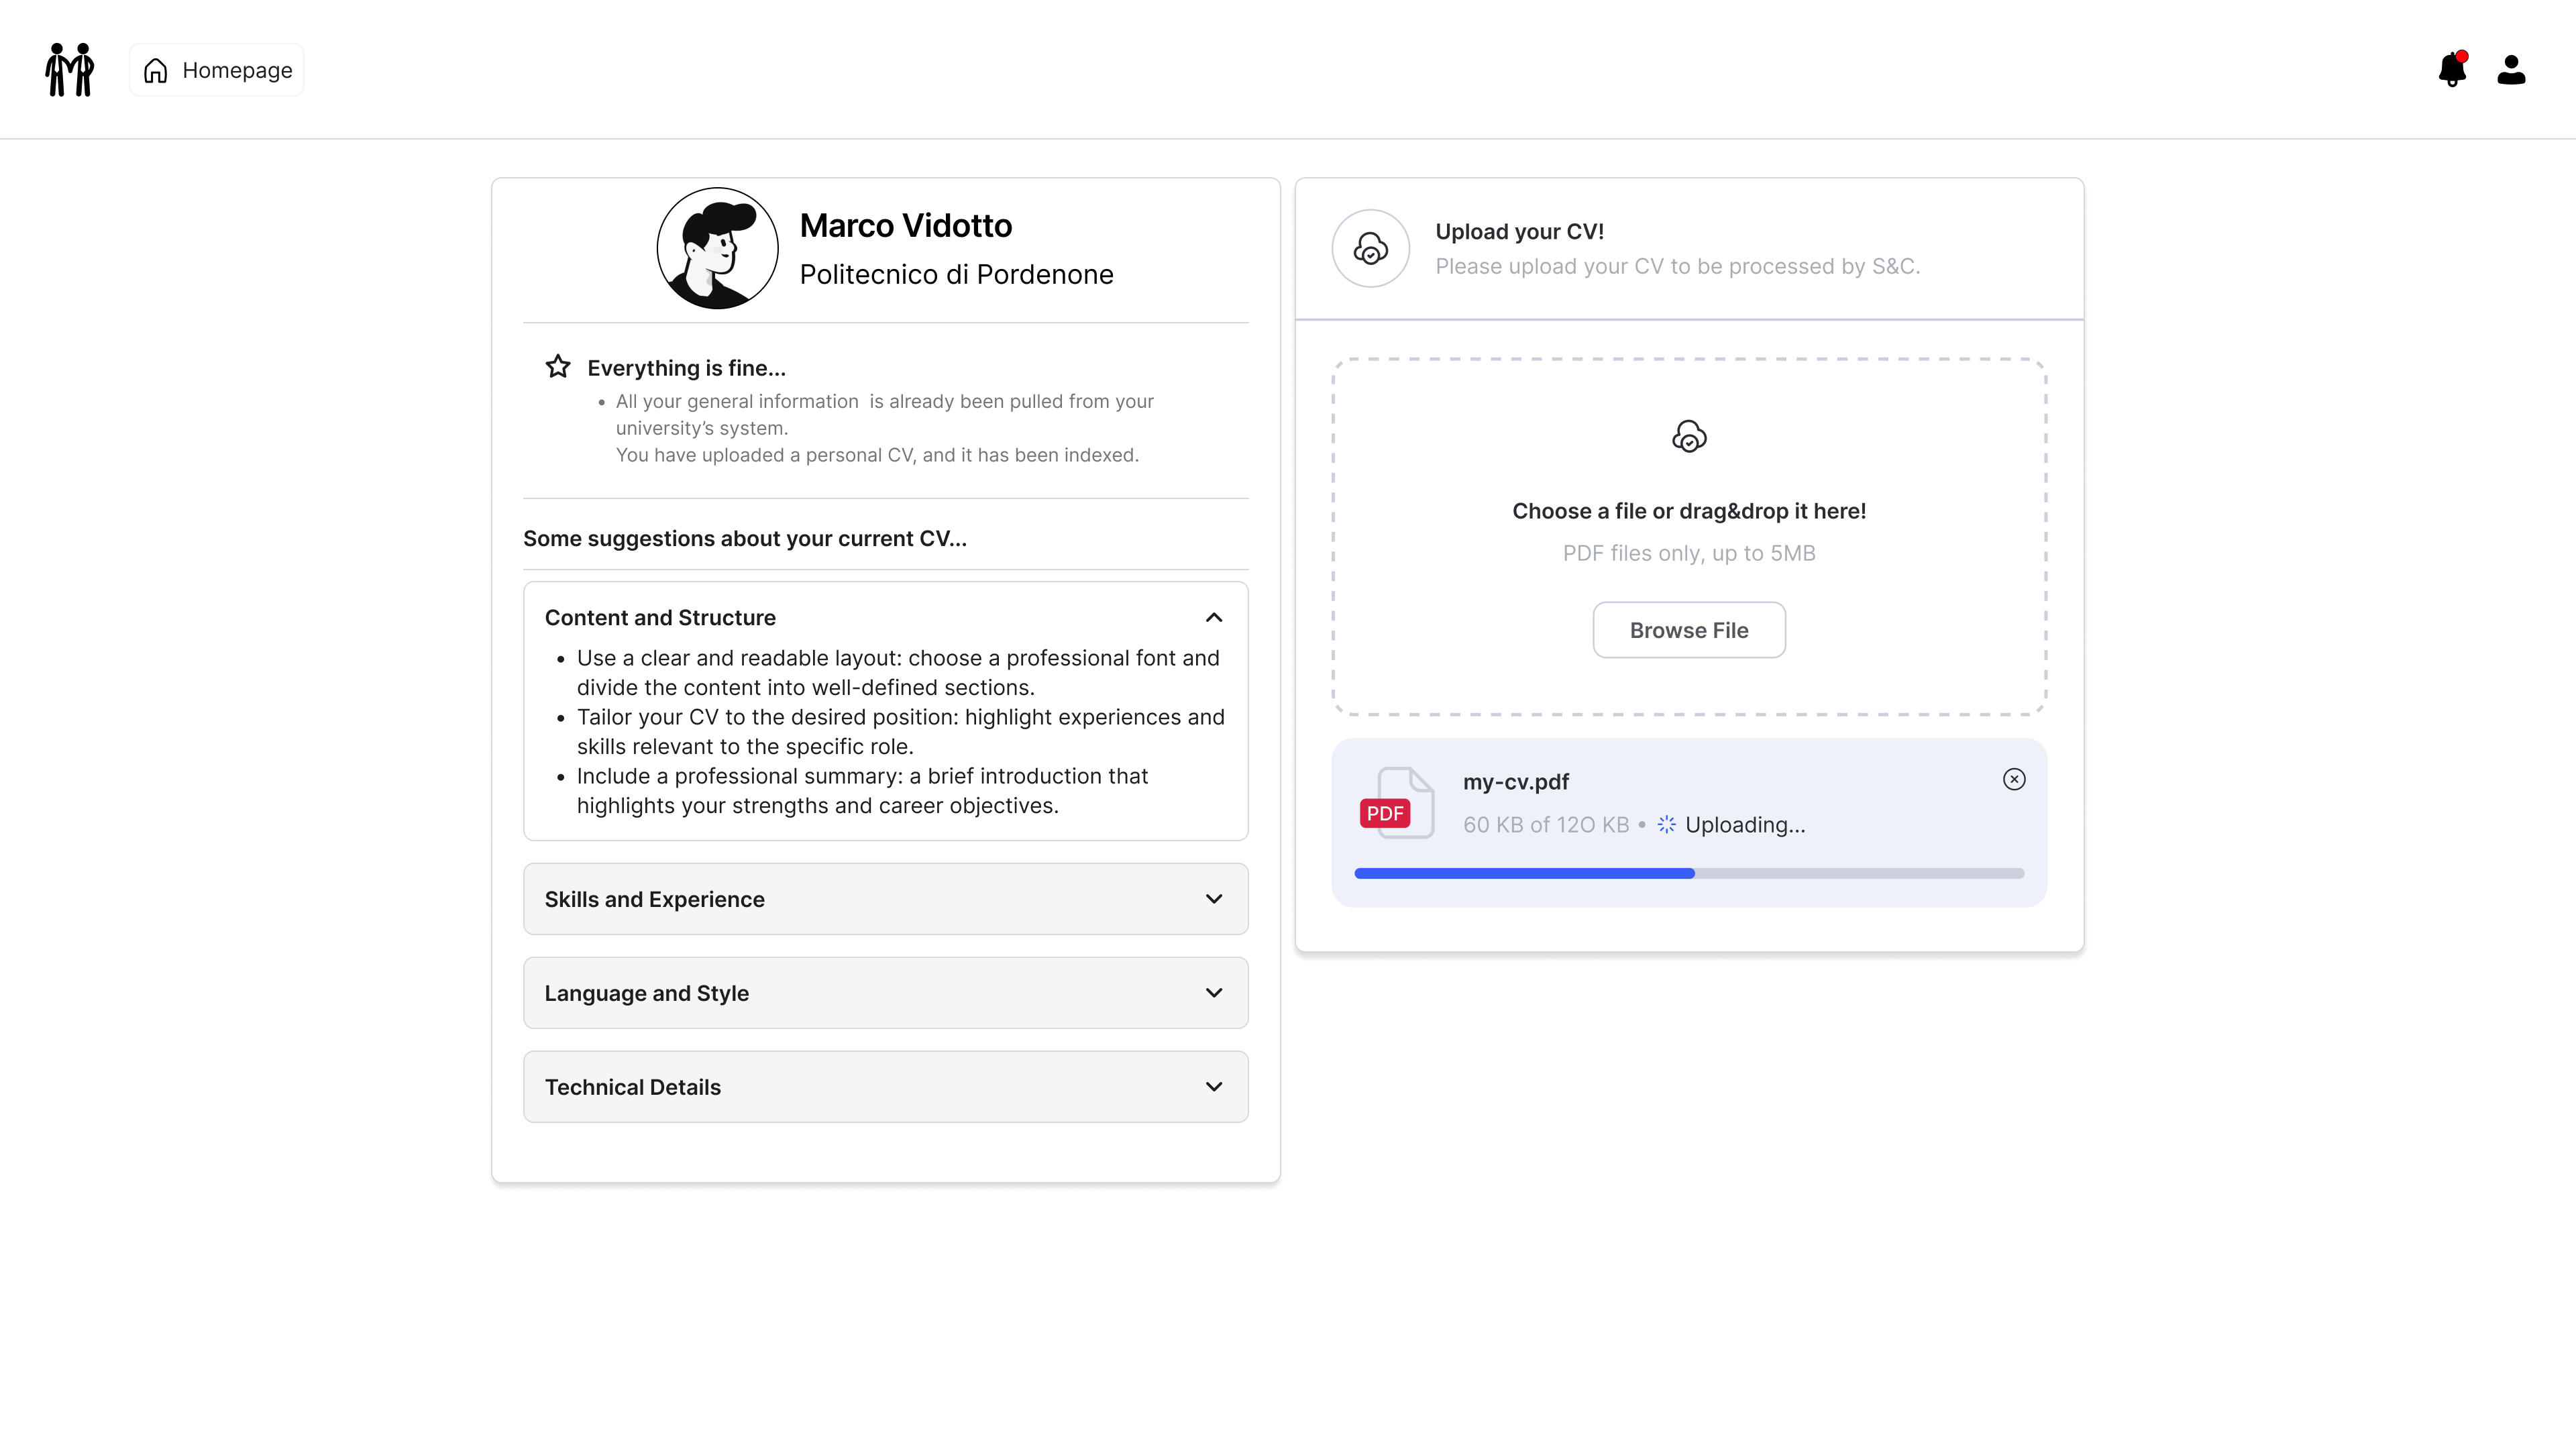
\includegraphics[width=1.0\textwidth]{Images/GUI/ST/Profile - ST.png}}
    \caption{"My Profile" - ST}
    \label{fig:profile-st}
\end{figure}

\par The "My Profile" page allows the ST to update their personal information by uploading a new CV (PDF only!).
Suggestions on how to improve the CV are also provided and will updated based on the processed CV's data.

\subsection{Internship Details - ST}

\begin{figure}[H]
    \centering
    \fbox{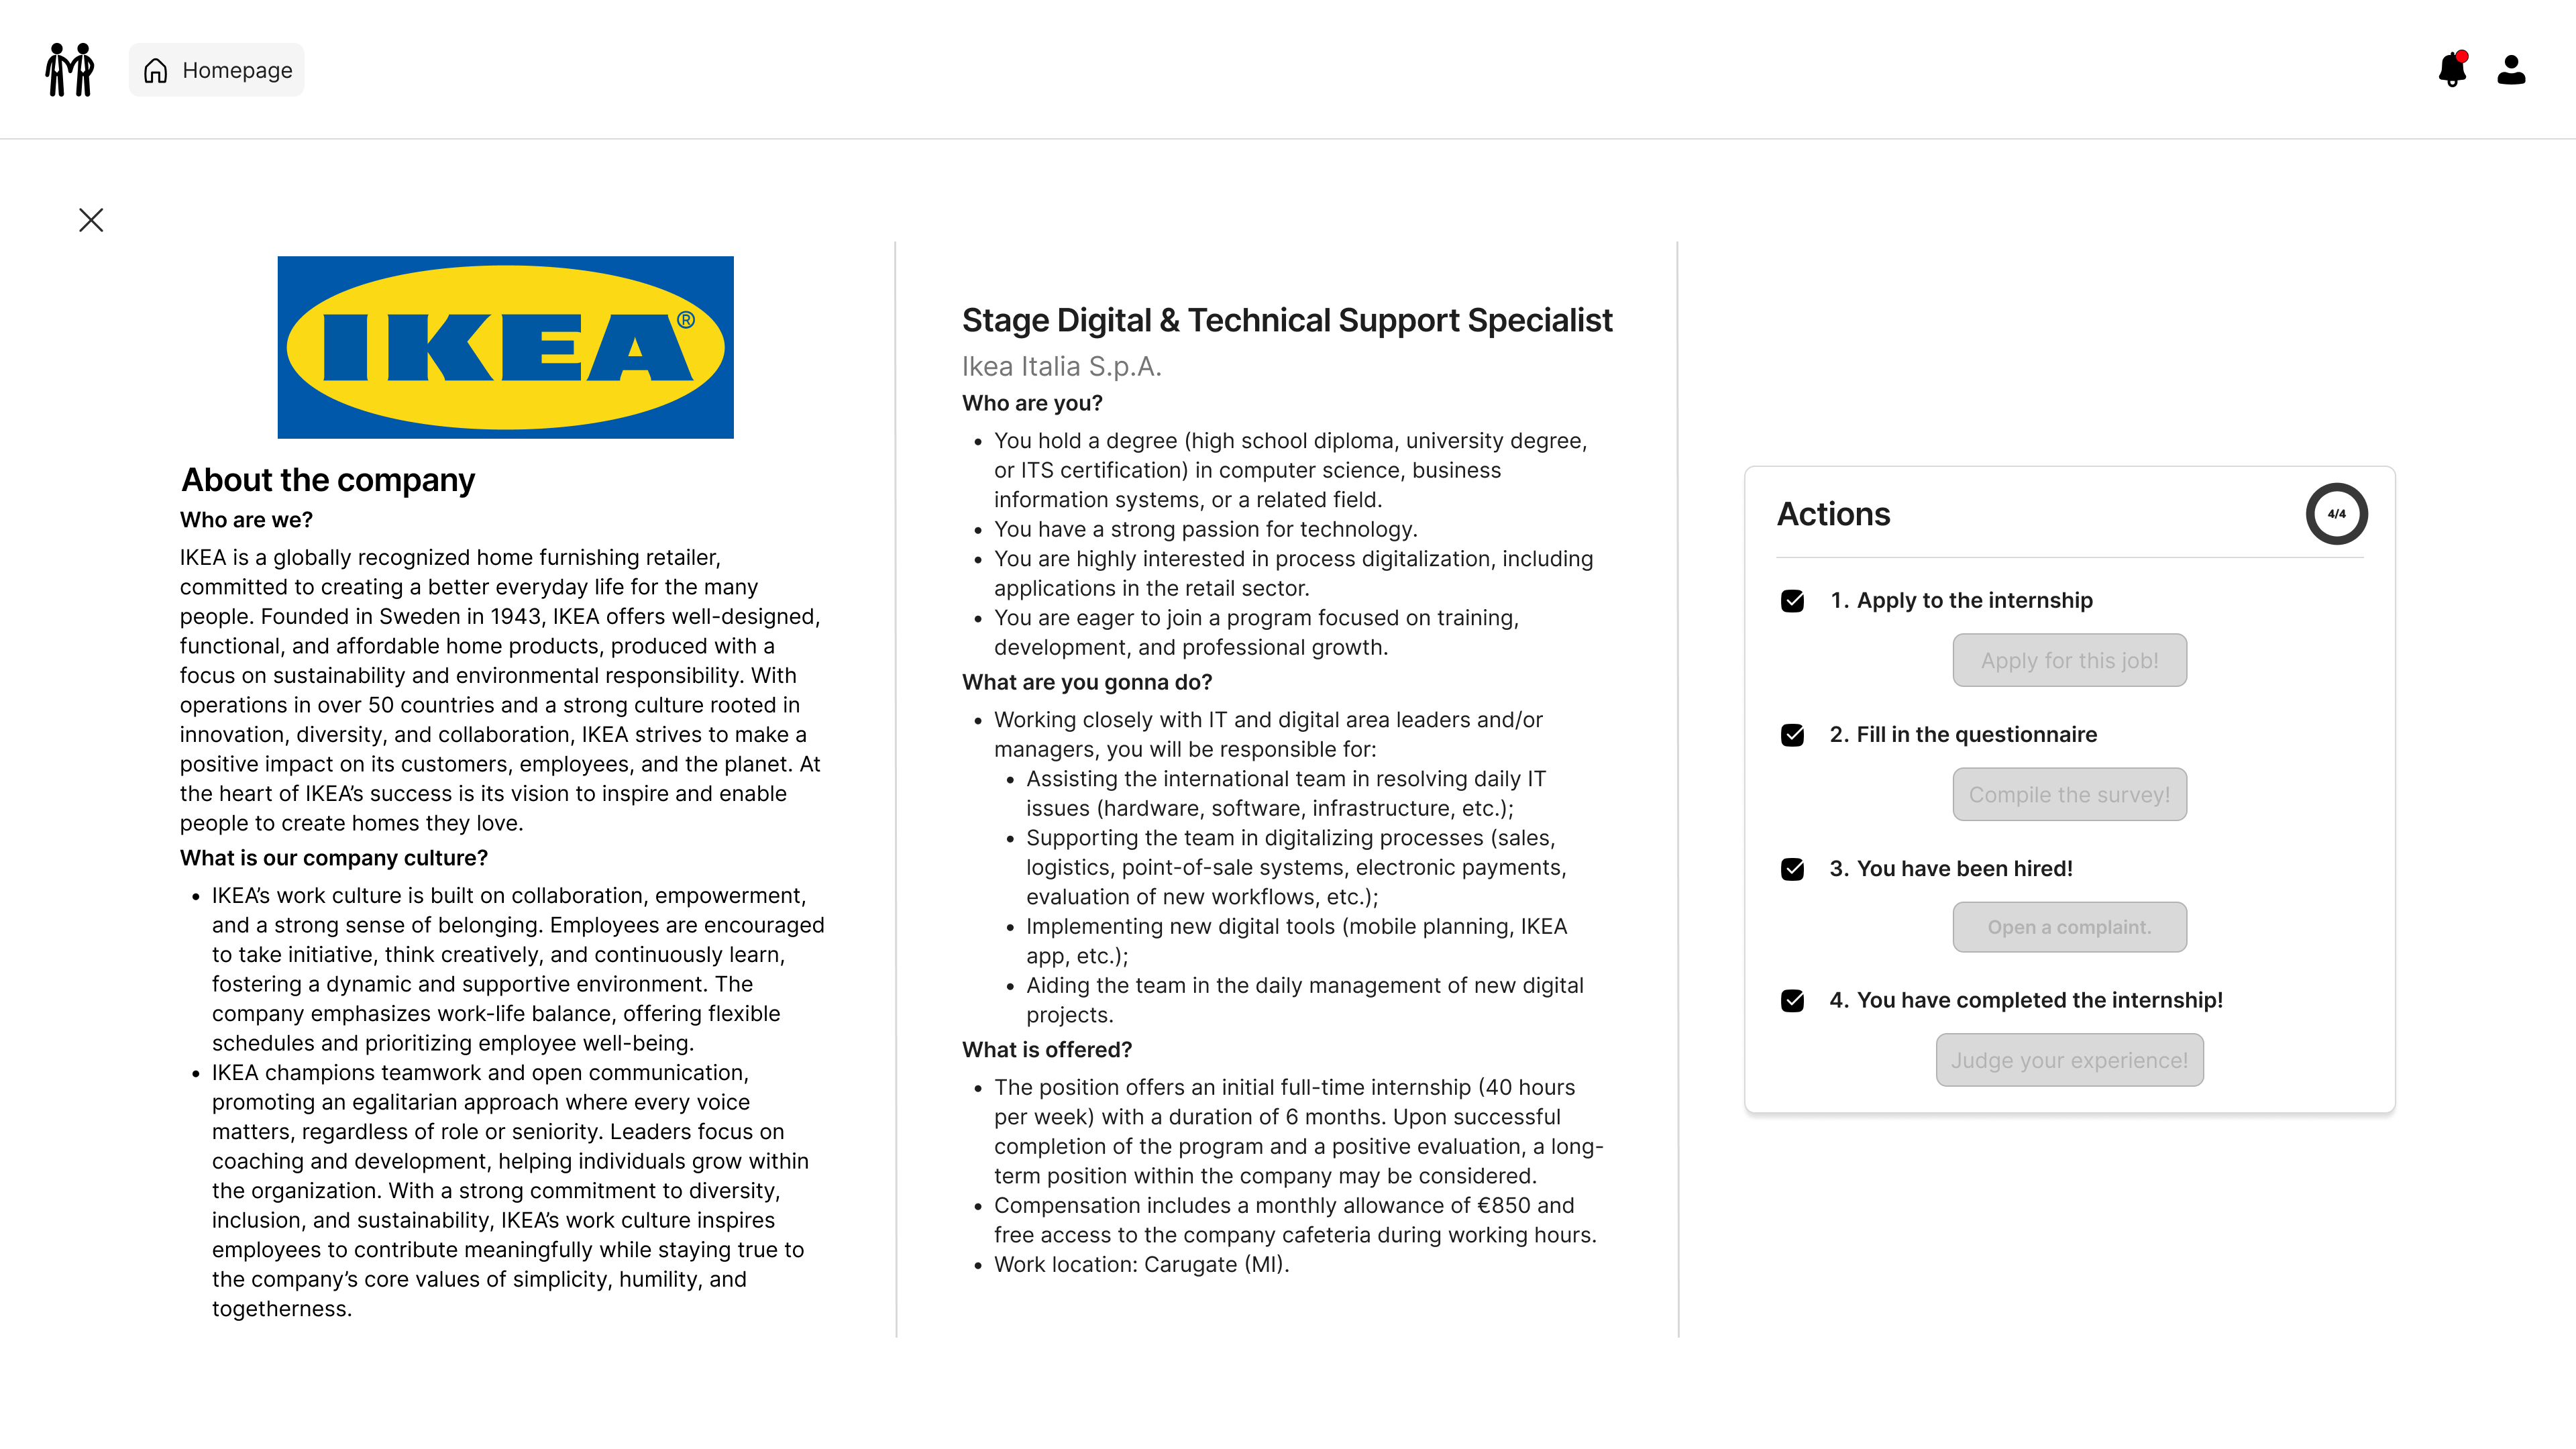
\includegraphics[width=1.0\textwidth]{Images/GUI/ST/Internship Details - Completed - ST.png}}
    \caption{Internship Details - ST}
    \label{fig:internship-details-st}
\end{figure}

\par The Internship Details page allows the ST to view all the details of an internship and the company that is
offering it. The ST can apply for the internship, access the Profiling Questionnaire, report violations using the
Issue Reporting Form and, once the internship is over, access the Internship Feedback Survey.

\par The various functions are enabled or disabled based on the status of the internship. A progress bar is also
present to show the progression of the hiring process.

\par For simplicity, here is presented the page for a completed internship; from this example will it be easy to infer
how the page will look like for all the various stages of the hiring process.

\subsection{Profiling Questionnaire - ST}
\label{subsec:profiling-questionnaire-st}%

\begin{figure}[H]
    \centering
    \fbox{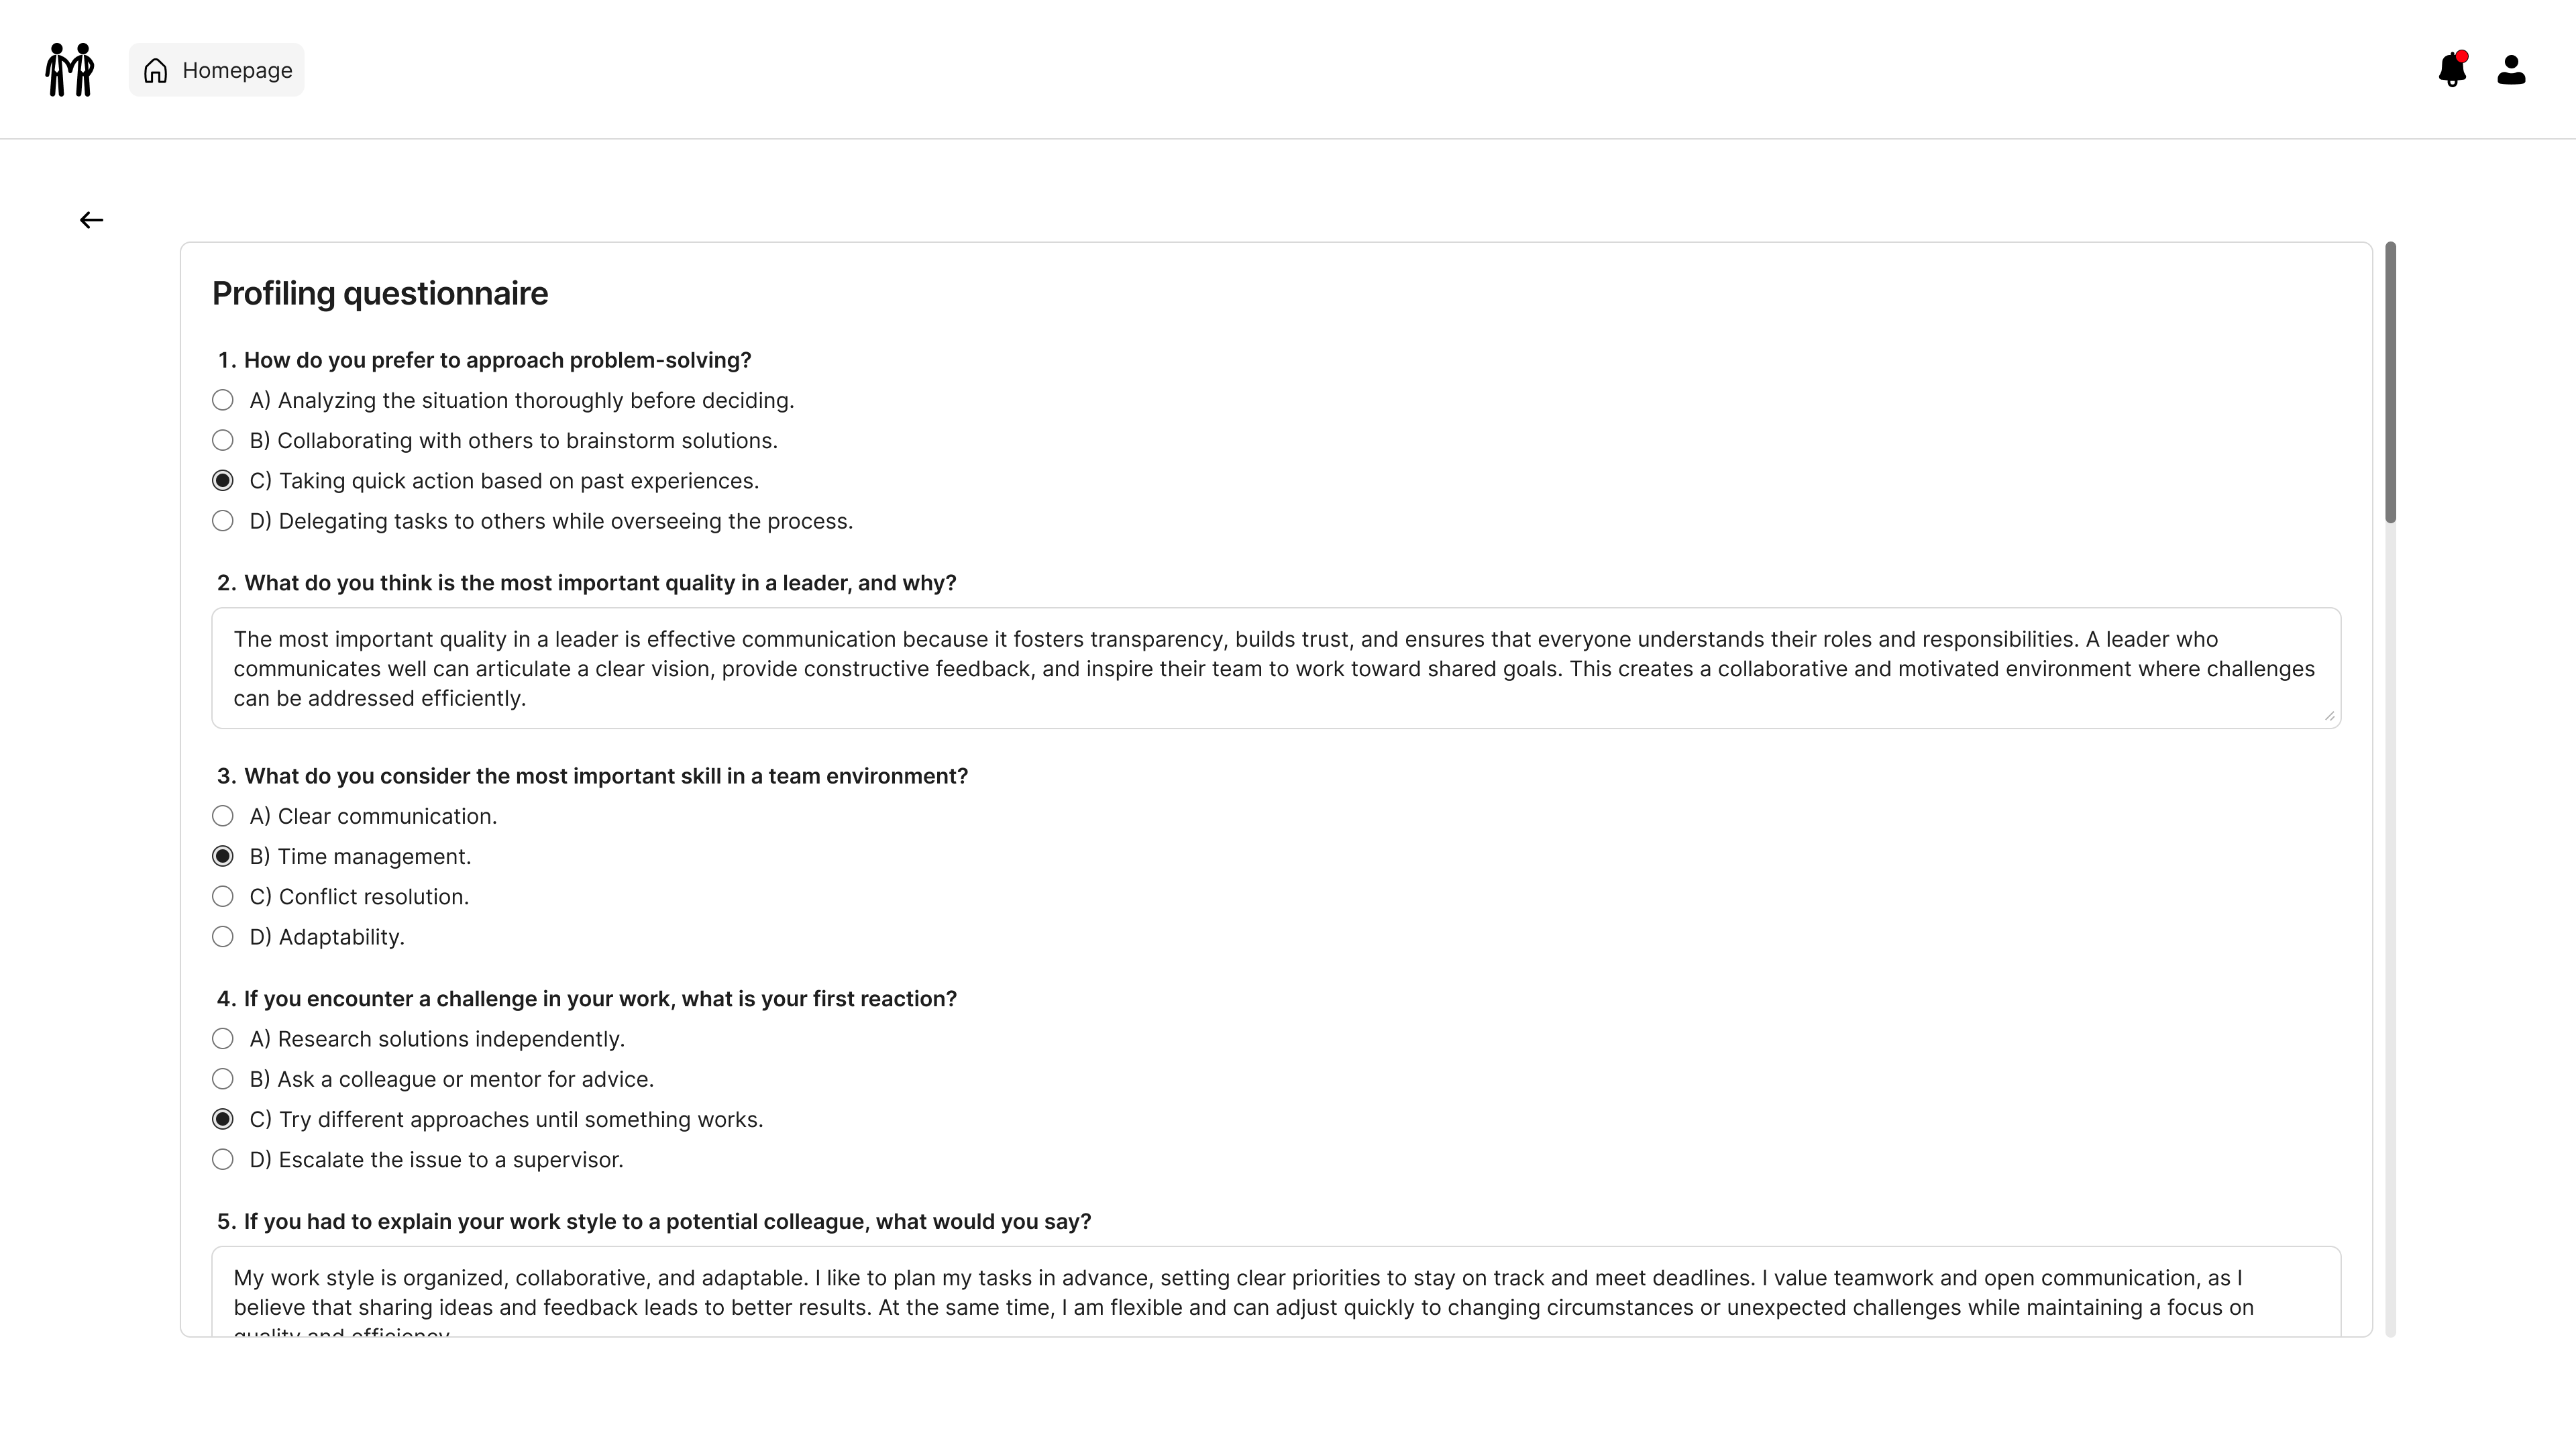
\includegraphics[width=1.0\textwidth]{Images/GUI/ST/Profiling Questionnaire - ST.png}}
    \caption{Profiling Questionnaire - ST}
    \label{fig:profiling-questionnaire-st}
\end{figure}

\par The Profiling Questionnaire page allows the ST to fill in a questionnaire to provide the company with more
information about themselves. The various questions will be automatically graded by the system to provide the
company with a synthetic evaluation of the ST. The questions will be provided manually by the CO.

\par A ST can only fill in the questionnaire only if they have been selected by the CO. This is de-facto the first
filtering step of the hiring process.

\subsection{Issue Reporting Form - ST}
\label{subsec:issue-reporting-form-st}%

\begin{figure}[H]
    \centering
    \fbox{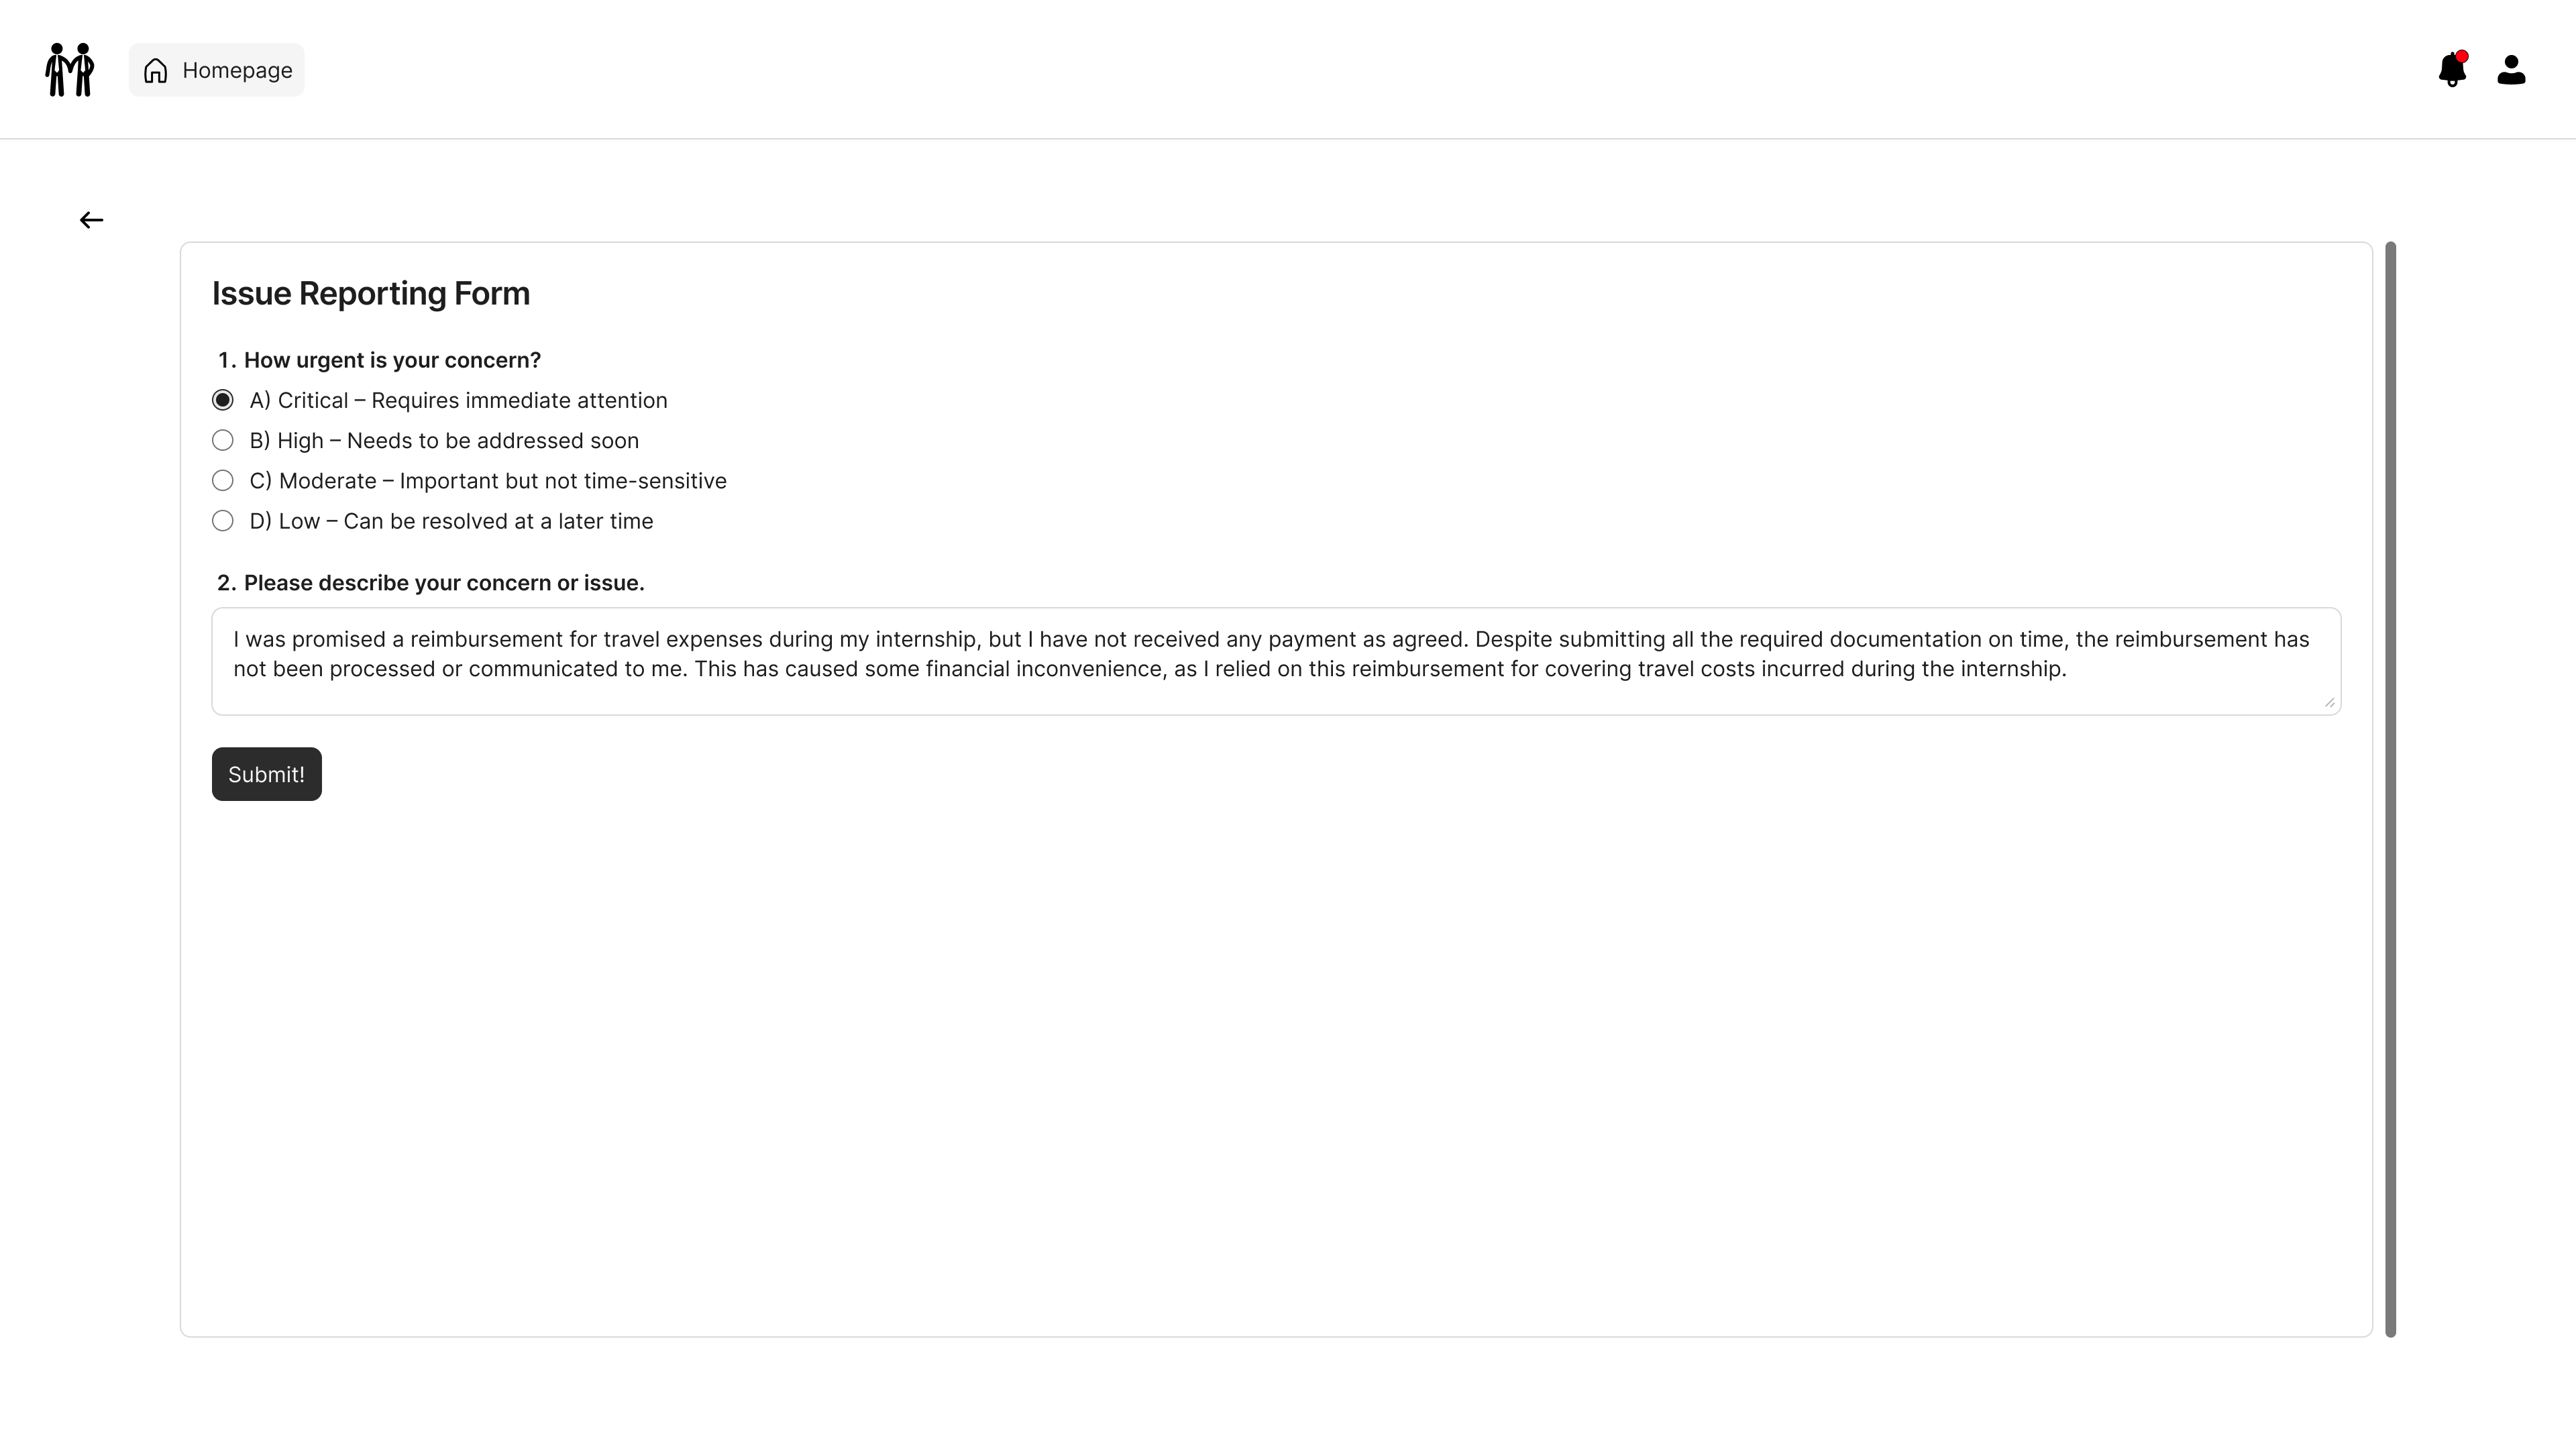
\includegraphics[width=1.0\textwidth]{Images/GUI/ST/Issue Reporting Form - ST.png}}
    \caption{Issue Reporting Form - ST}
    \label{fig:issue-reporting-form-st}
\end{figure}

\par The Issue Reporting Form page allows the ST to report any violations they have encountered during the
internship. The form is simple and allows the user to provide a description of the violation and any evidence they
have. The form is then sent to the company and the UN to evaluate the situation.

\par The user himself can choose the urgency of their issue.

\subsection{Internship Feedback Survey - ST}
\label{subsec:internship-feedback-survey-st}%

\begin{figure}[H]
    \centering
    \fbox{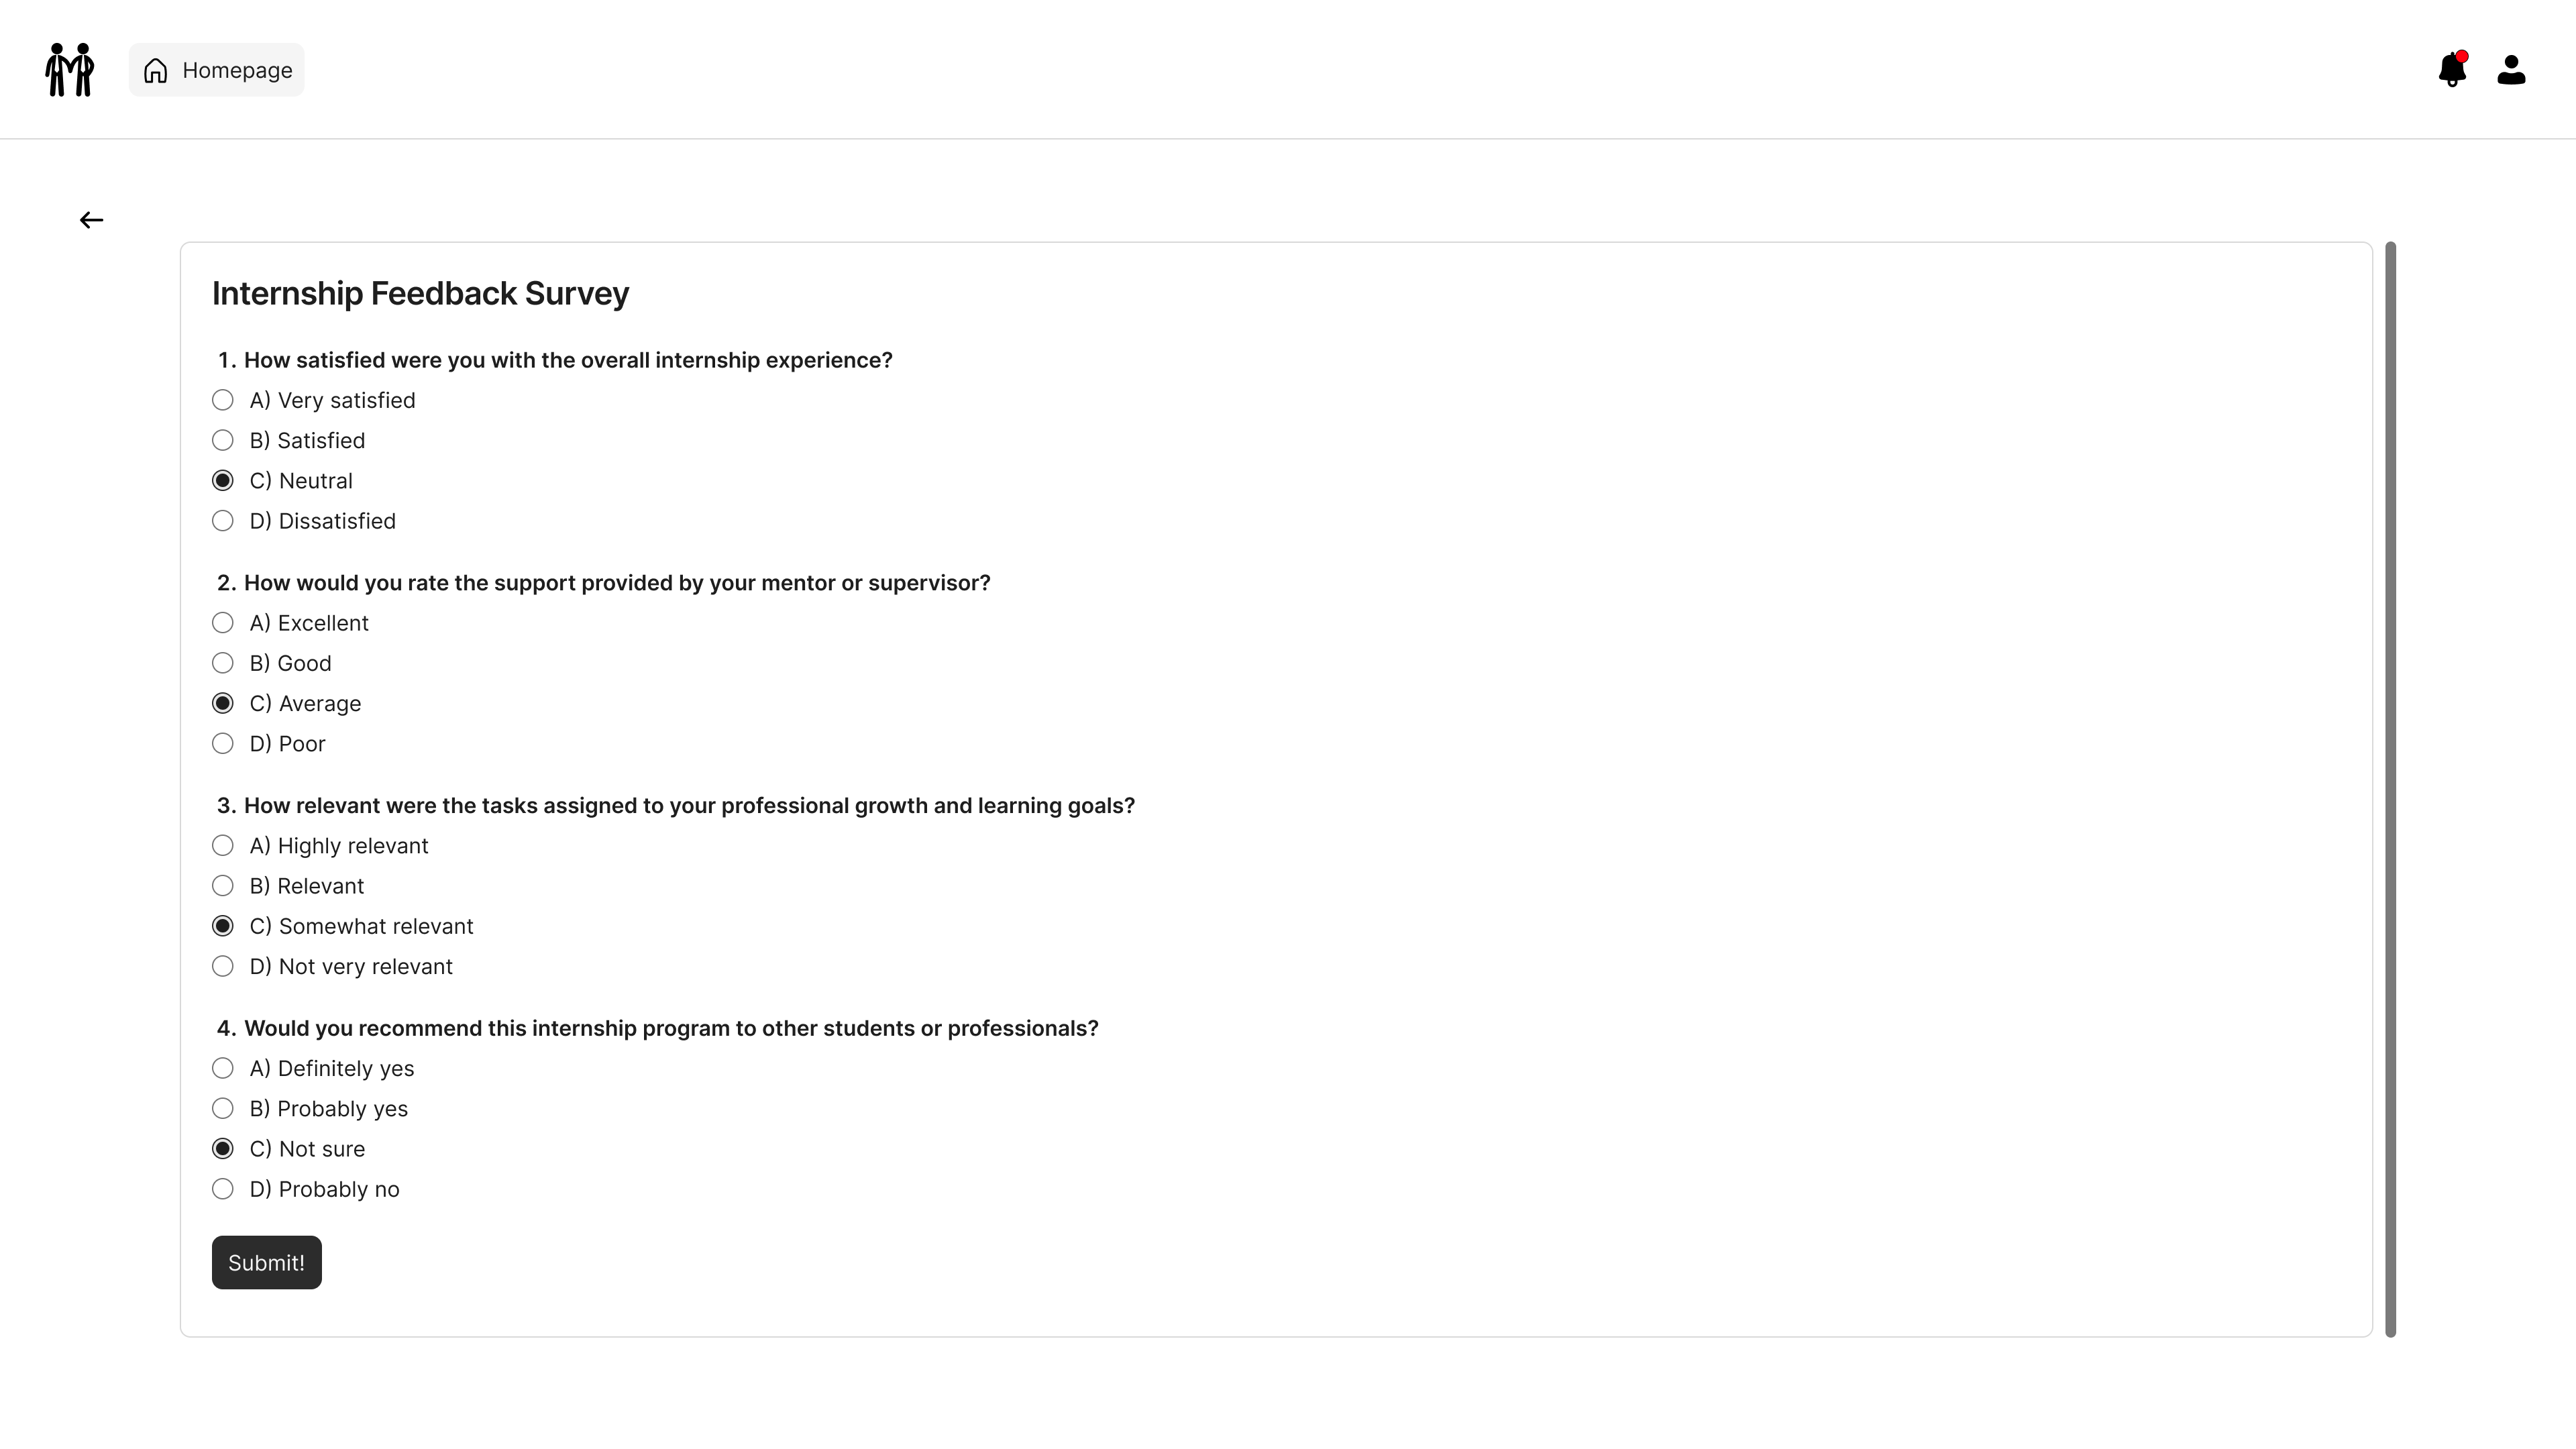
\includegraphics[width=1.0\textwidth]{Images/GUI/ST/Internship Feedback Survey - ST.png}}
    \caption{Internship Feedback Survey - ST}
    \label{fig:internship-feedback-survey-st}
\end{figure}

\par The Internship Feedback Survey page allows the ST to provide a final evaluation on the internship. S\&C and UN
will use this information to improve the quality of the internships and the platform.

\section{User Flow: CO}
\label{sec:user-flow-co}%

\begin{figure}[H]
    \centering
    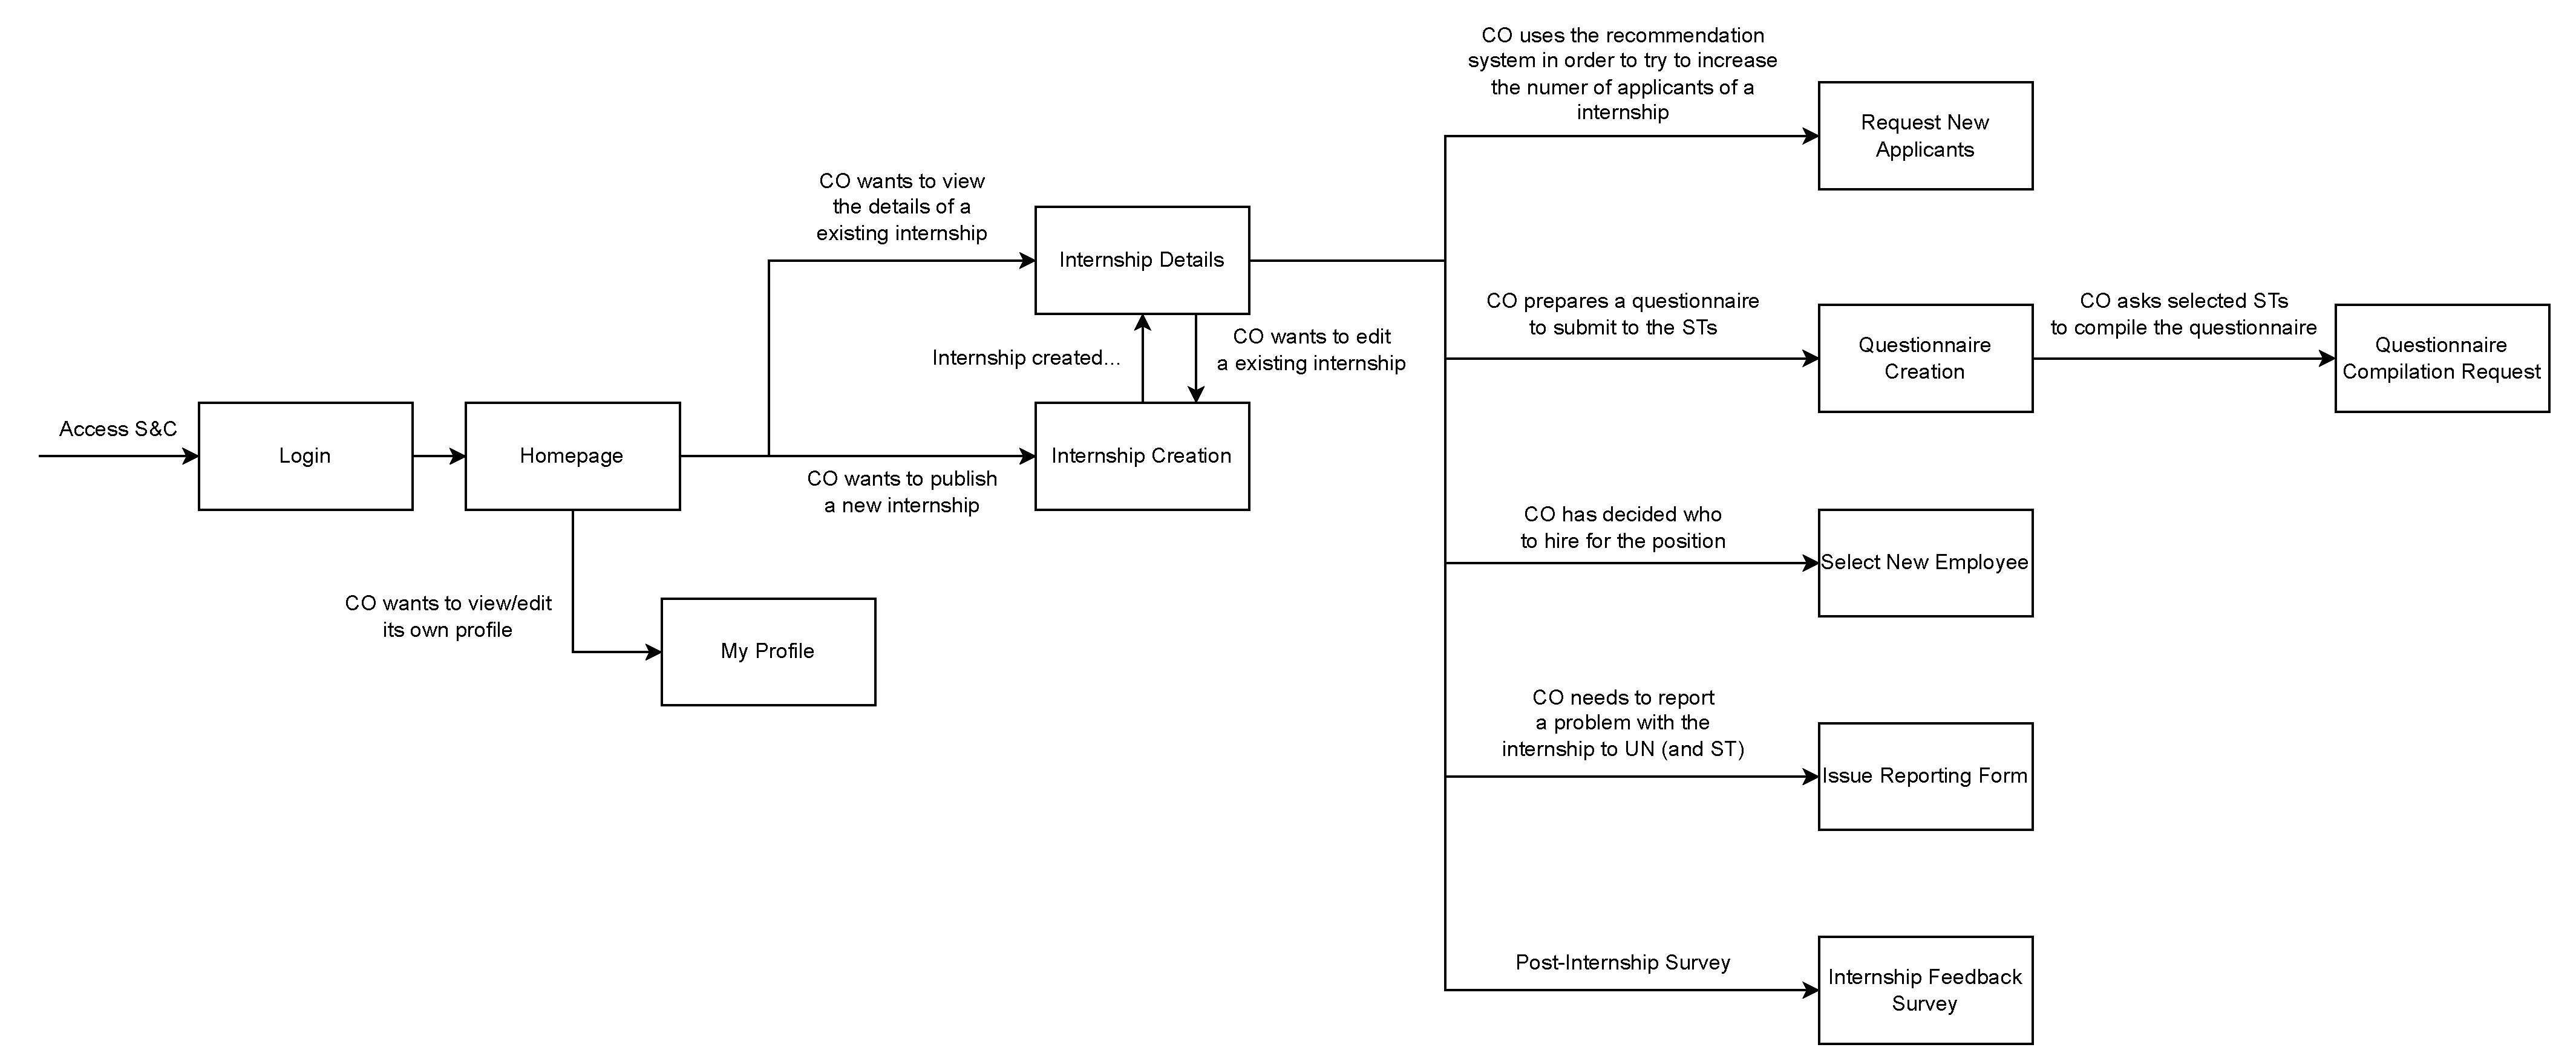
\includegraphics[width=1.0\textwidth]{Images/GUI/CO/Diagram.pdf}
    \caption{CO User Flow Diagram}
    \label{fig:co-user-flow-diagram}
\end{figure}

\par Now is presented the user flow diagram for the CO. The CO uses the Login page to authenticate and access S\&C
using plain credentials provided by S\&C's administrators. Once logged in, the CO is redirected to the Homepage, here
the user can view all the internships they have posted (past and present) and view their details (Internship Details).
The Login page is the same for all the users and as such will not be presented again.

\par On the Internship Details page, the CO can view all the details of the internship, edit them - up until the
application deadline - and send notifications to the STs that the system has deemed as a good match for the internship
(more details will be provided later). After the application deadline, the CO can create the questionnaire
(Questionnaire Creation) to submit to the STs that the CO has selected - thus creating a first filter - using the
Questionnaire Compilation Request. Using the Select New Employee page the CO can view the results of said
questionnaire and select the ST that will be hired. Once the internship is over, the CO can access the Internship
Feedback Survey page to evaluate the internship. In case of issues, the CO can access the Issue Reporting Form page
to report them.

\par The creation of a new internship is done using the Internship Creation page also accessible from the Homepage: the
CO will be presented with a two-step form to fill in all the required information. Finally, the CO can access and
update their profile using the Profile page accessible from a button in the header.

\subsection{Homepage - CO}
\label{subsec:homepage-co}%

\begin{figure}[H]
    \centering
    \fbox{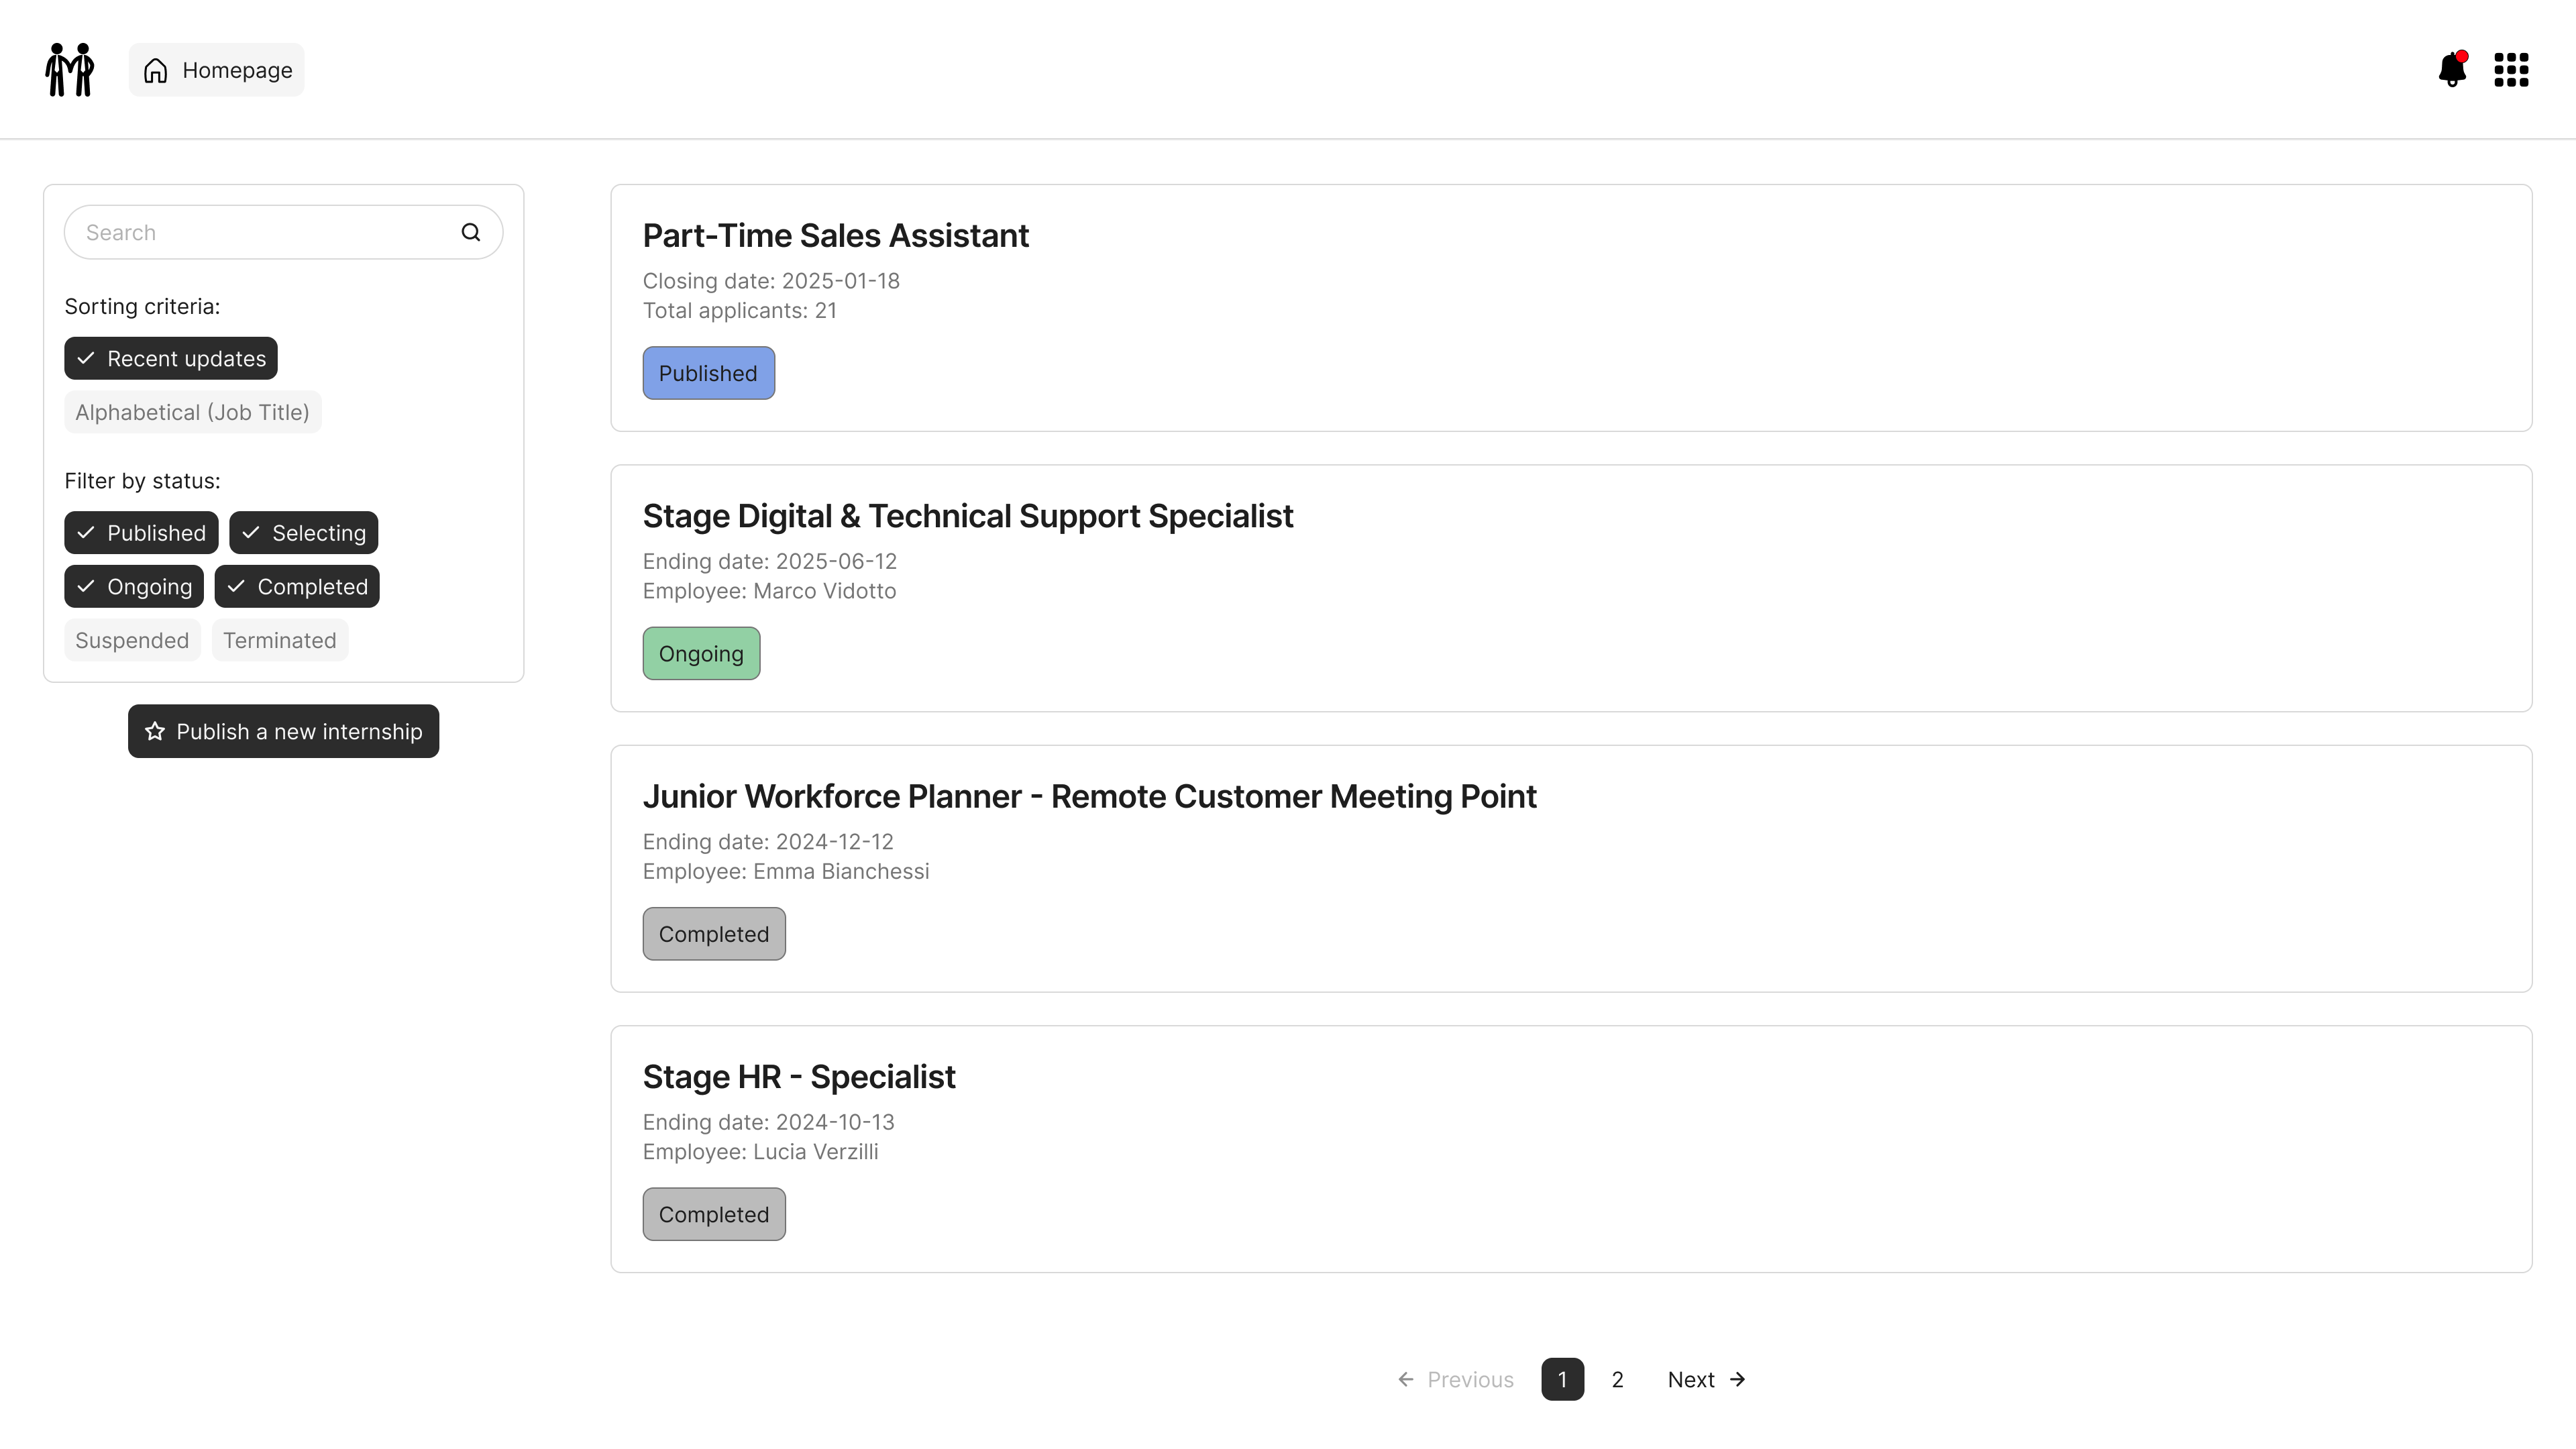
\includegraphics[width=1.0\textwidth]{Images/GUI/CO/Homepage - CO.png}}
    \caption{Homepage - CO}
    \label{fig:homepage-co}
\end{figure}

\par The Homepage is the main page for the CO. Here the user can view all the internships they have posted (past and
present) and view their details. Proper filters are provided to allow the user to search for internships based on
their preferences and needs. Also, in this page is present a button that allows the CO to create a new internship.

\par As all the other pages, the header is present and allows the user to: access their profile, log out from the
platform and view any new notifications from the related submenu.

\begin{figure}[H]
    \centering
    \fbox{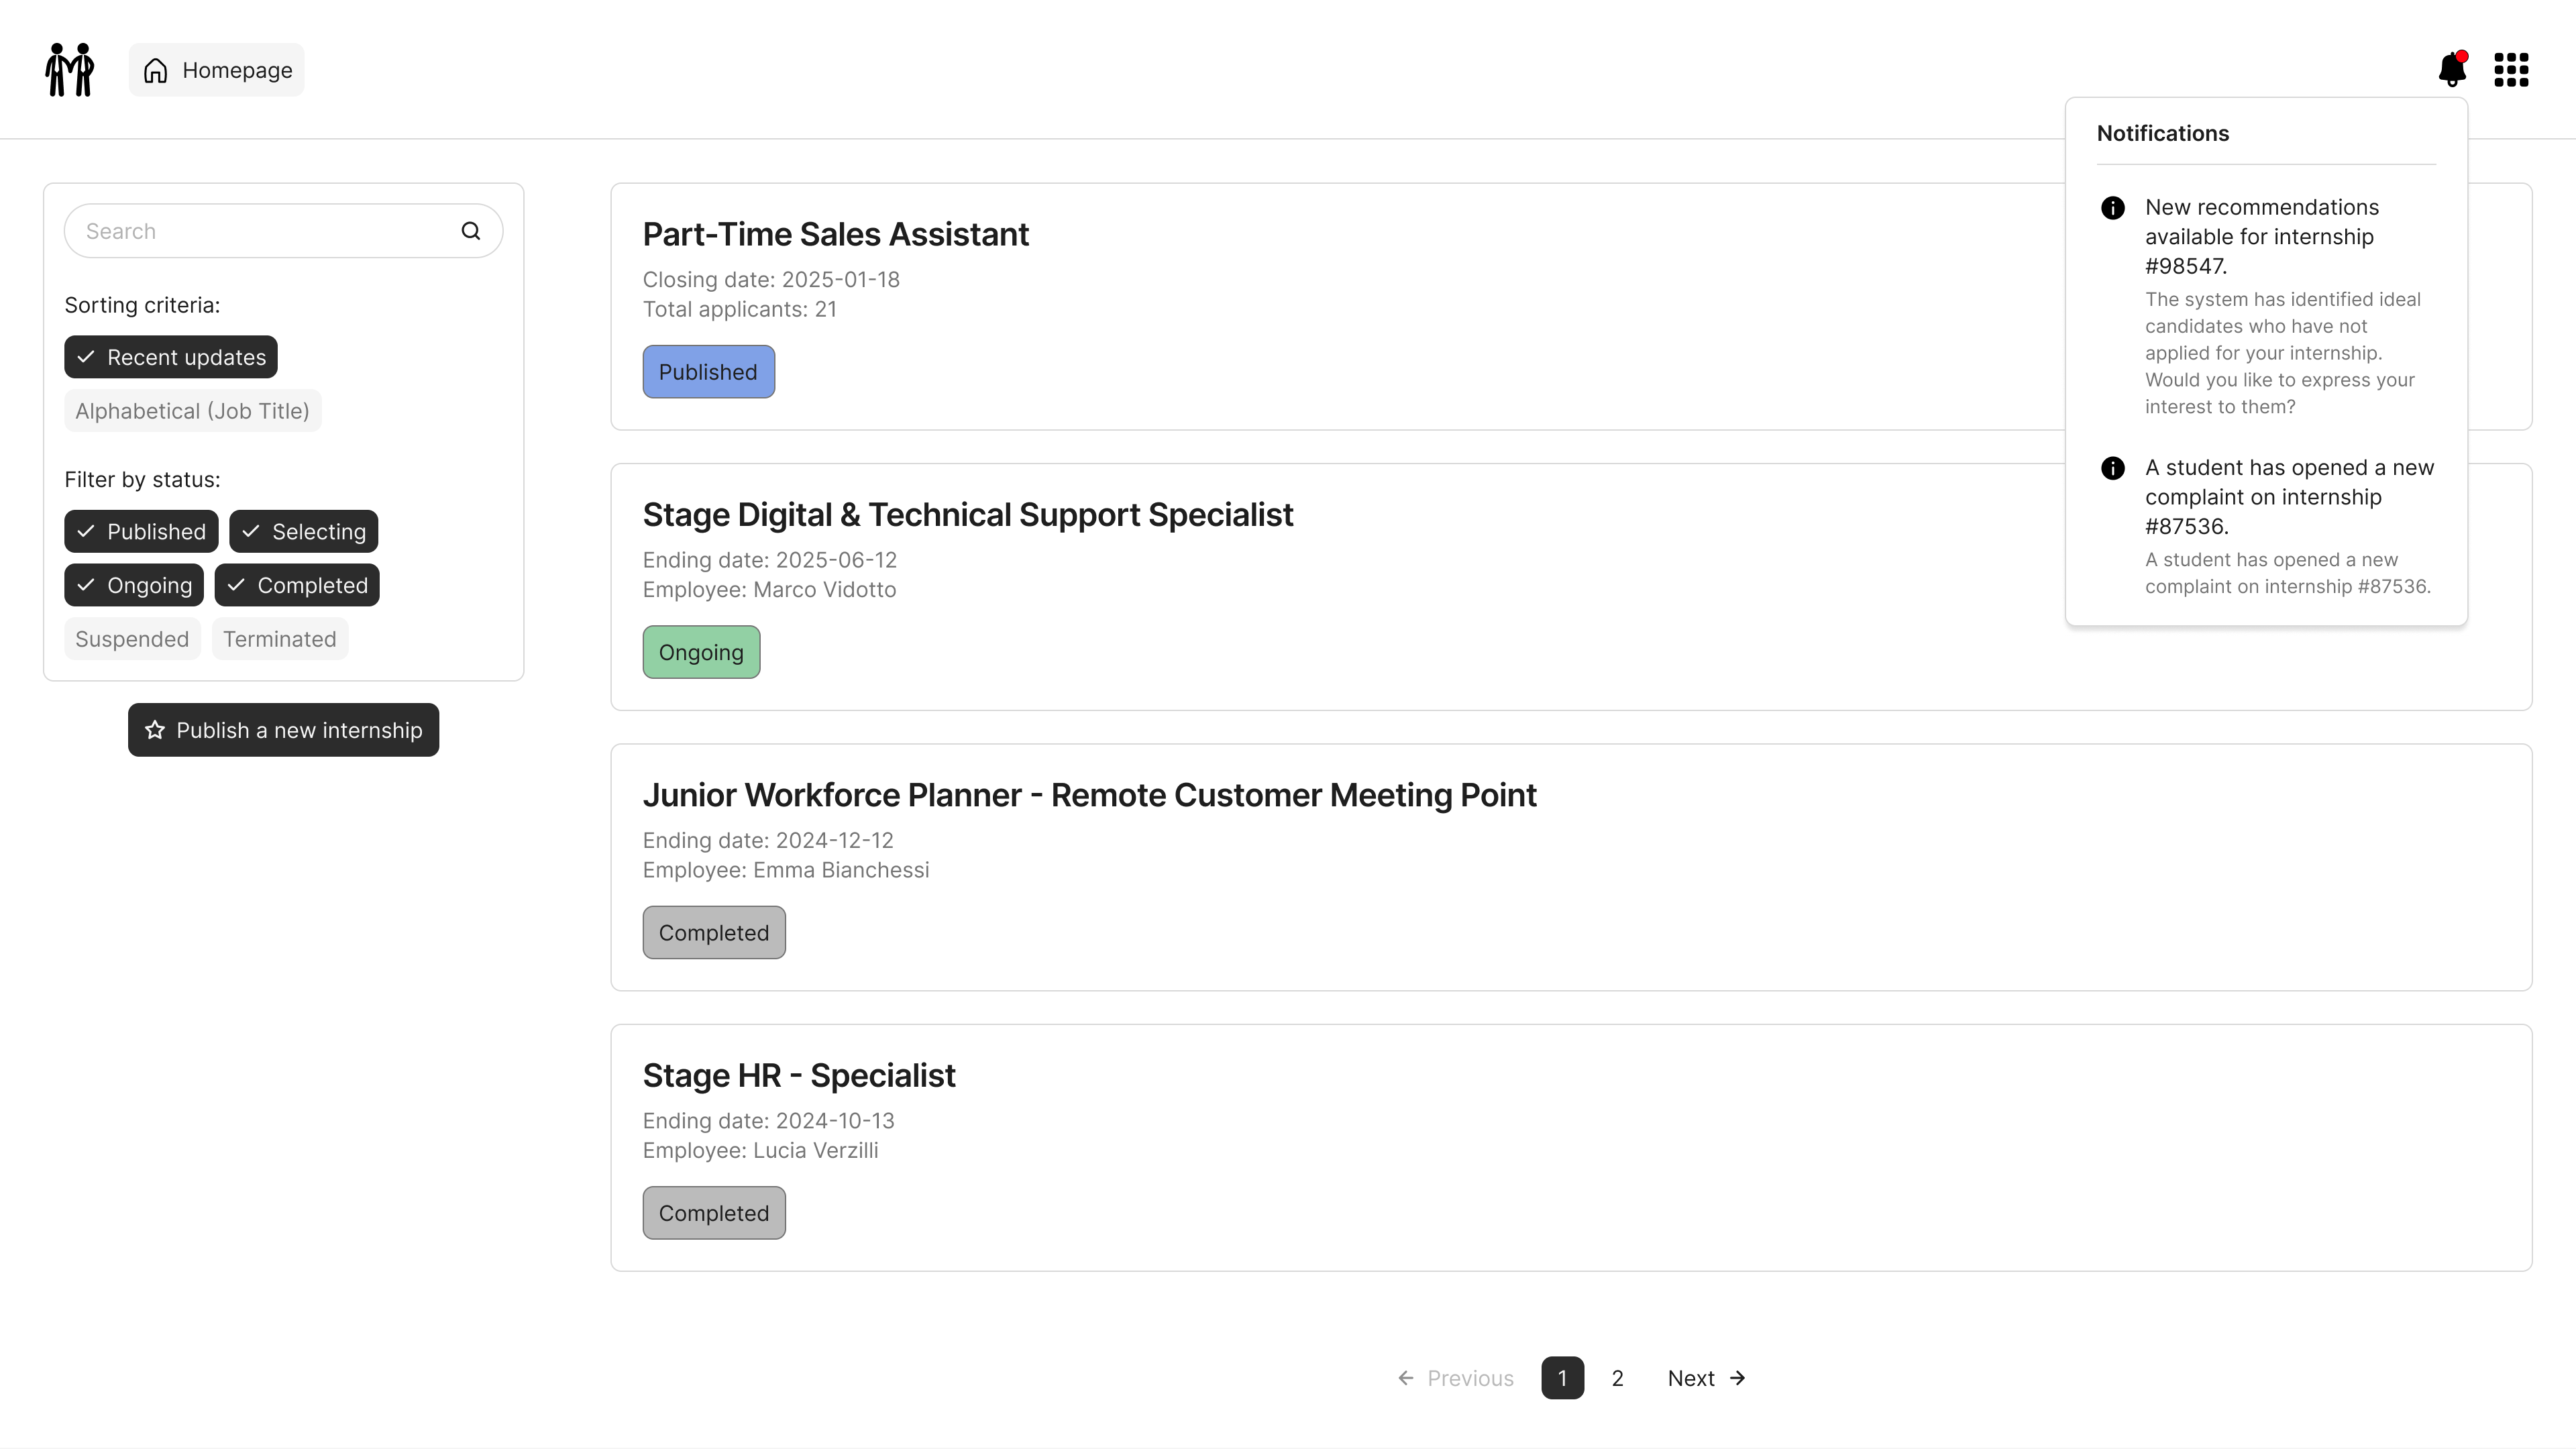
\includegraphics[width=1.0\textwidth]{Images/GUI/CO/Homepage - CO - Notification.png}}
    \caption{Homepage - CO - Notification}
    \label{fig:homepage-co-notification}
\end{figure}

\begin{figure}[H]
    \centering
    \fbox{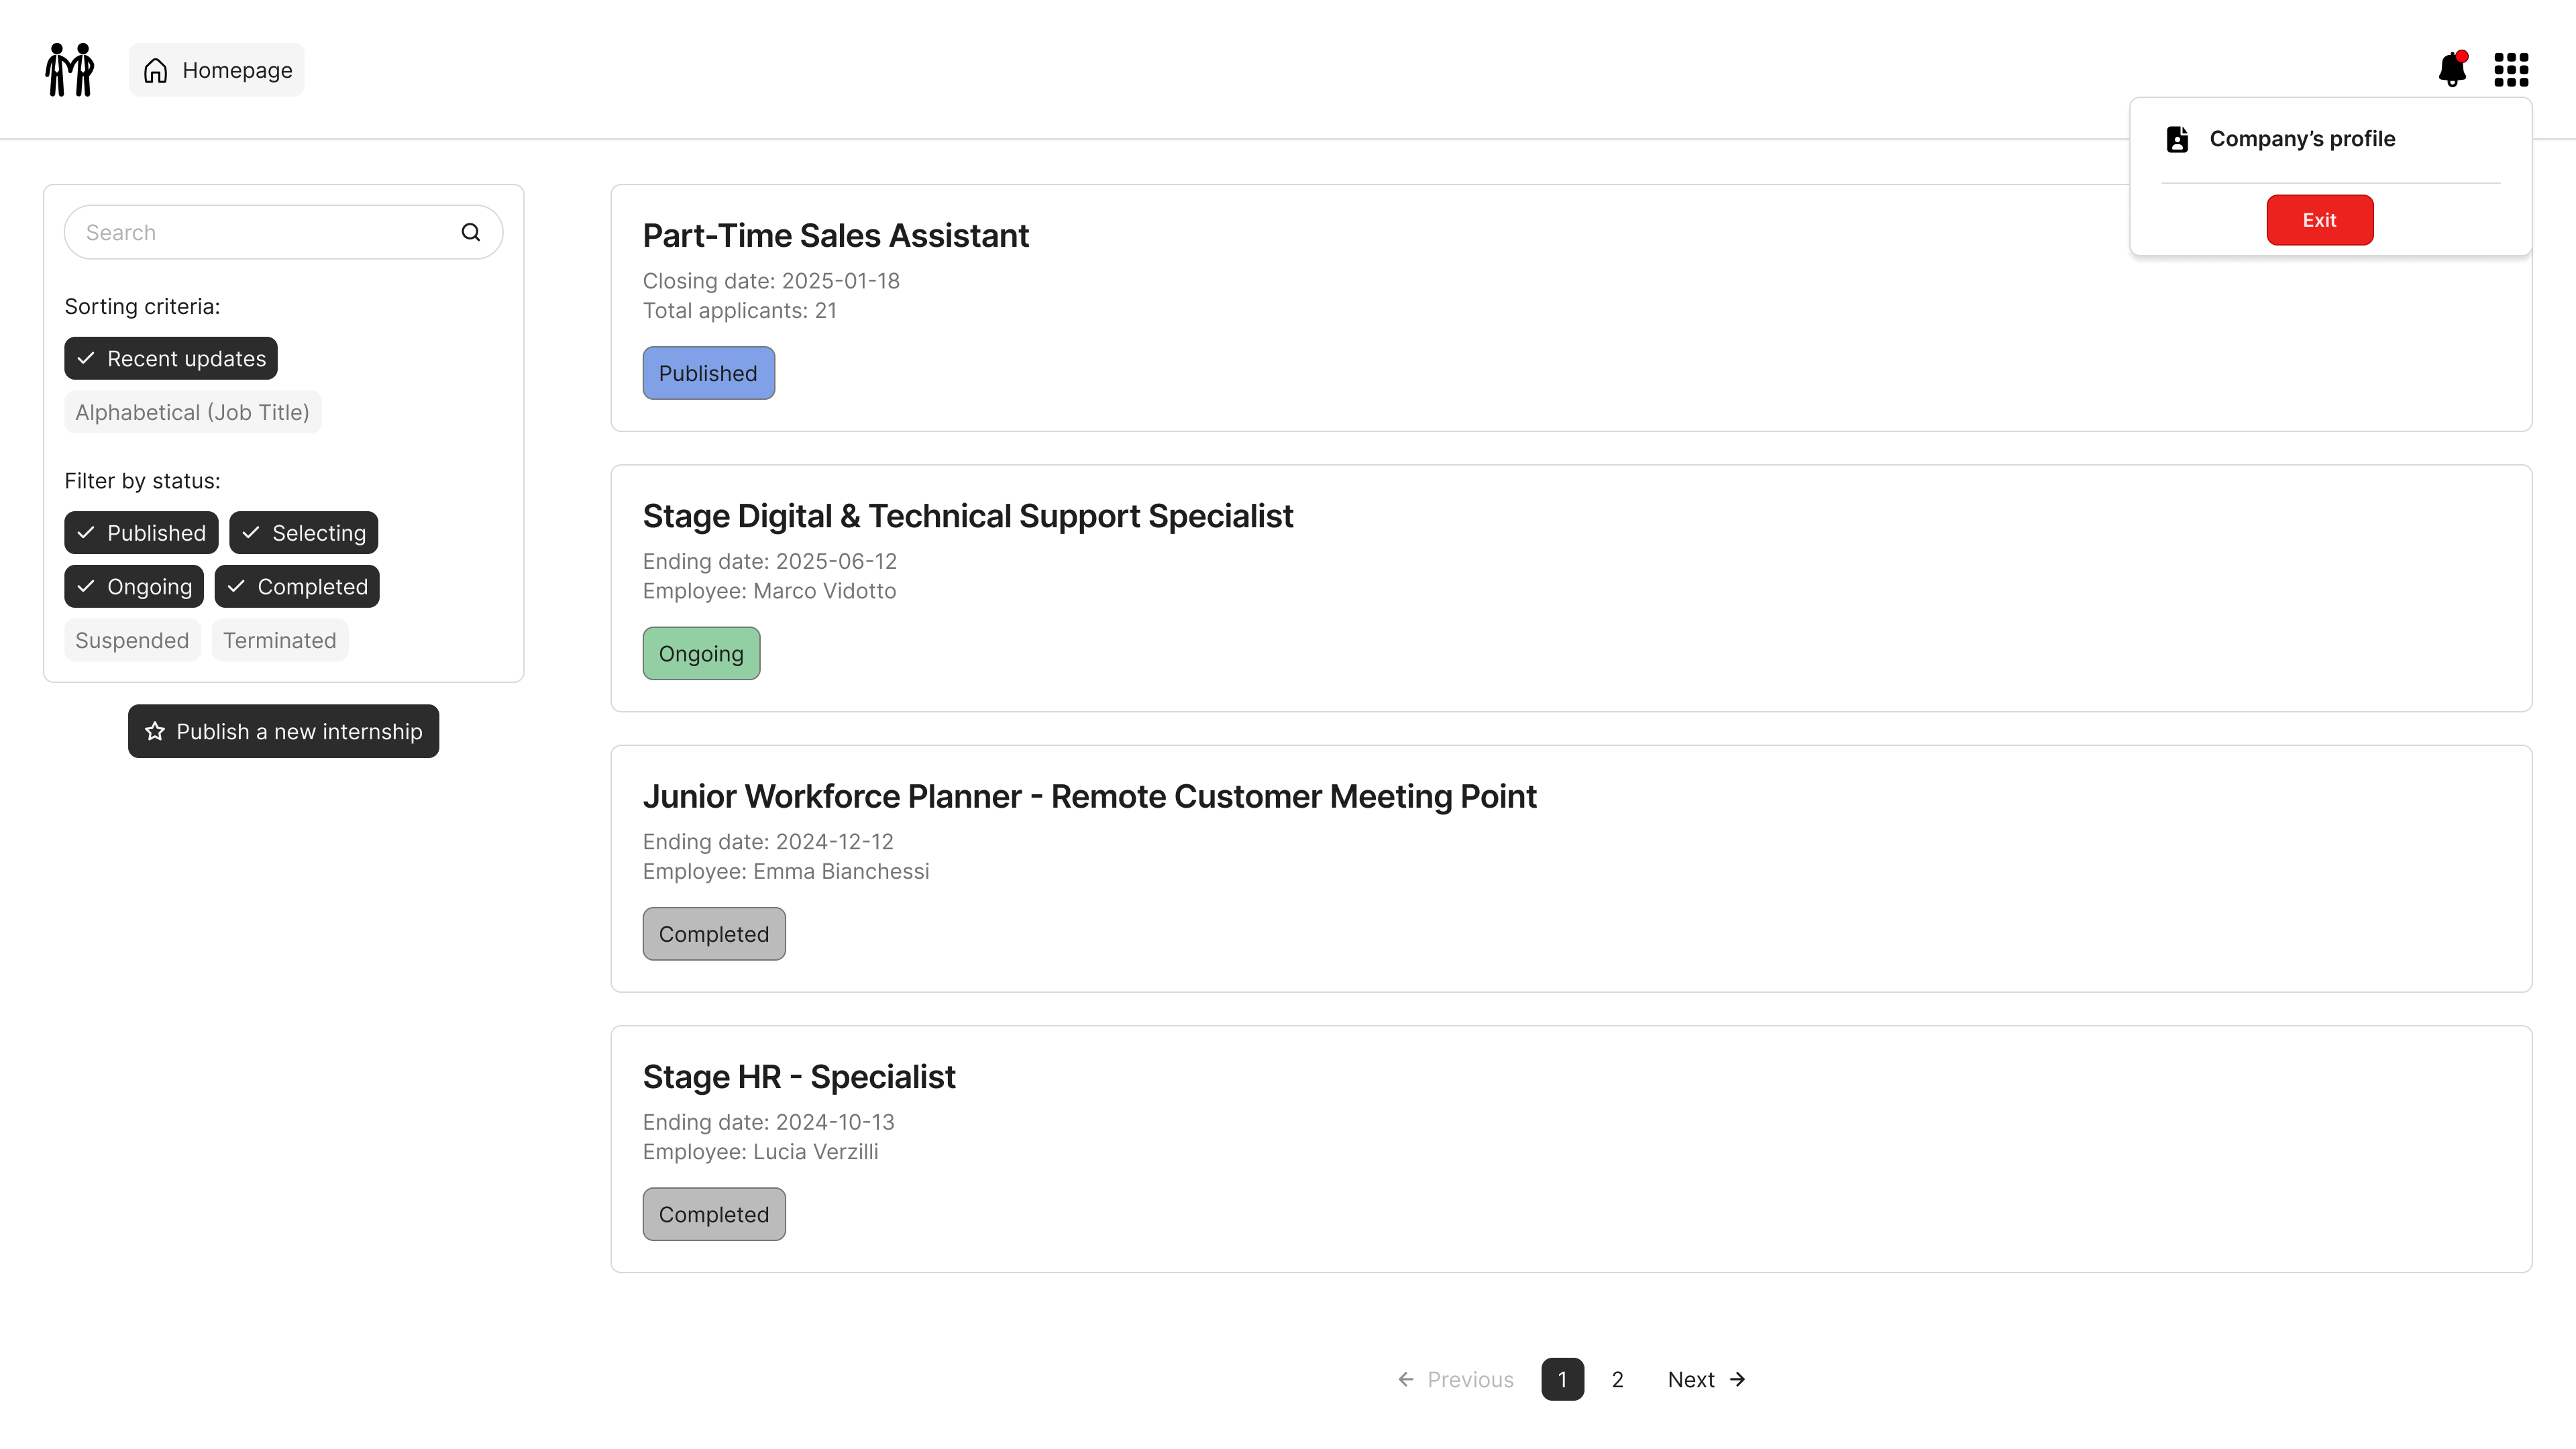
\includegraphics[width=1.0\textwidth]{Images/GUI/CO/Homepage - CO - Profile.png}}
    \caption{Homepage - CO - Profile}
    \label{fig:homepage-co-profile}
\end{figure}

\subsection{Internship Creation - CO}
\label{subsec:internship-creation-co}%

\begin{figure}[H]
    \centering
    \fbox{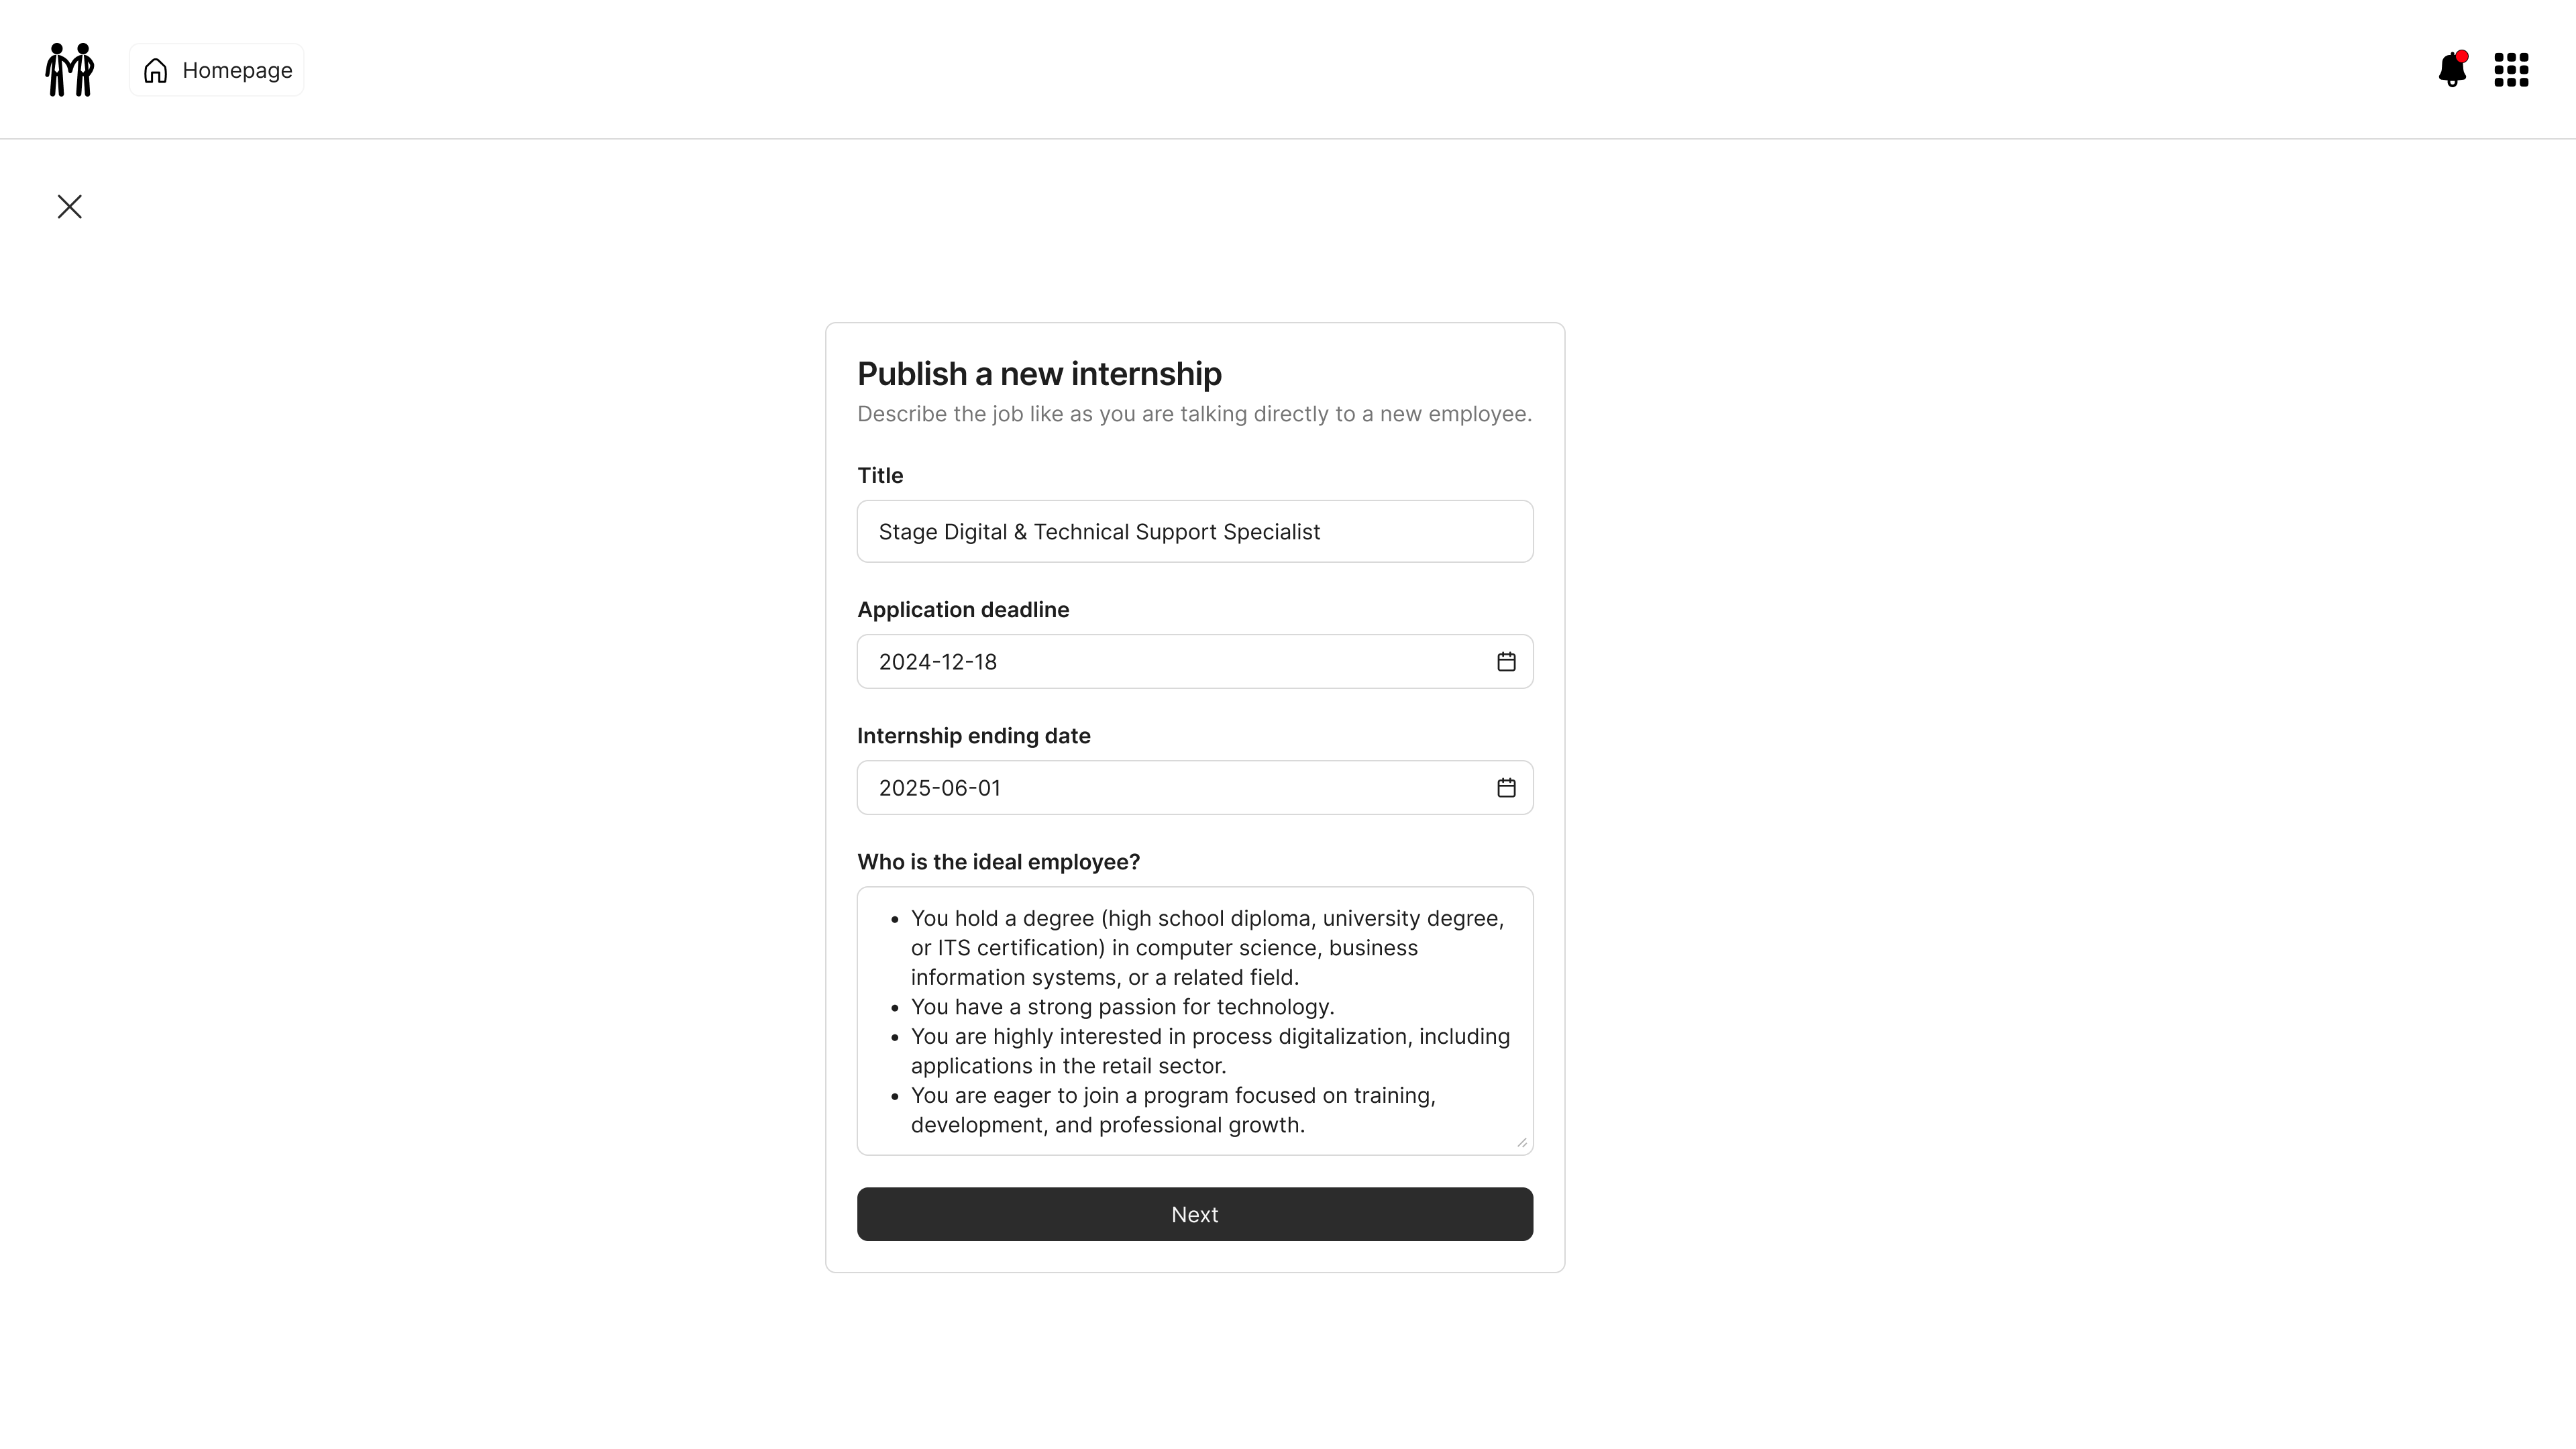
\includegraphics[width=1.0\textwidth]{Images/GUI/CO/Internship Creation - 1 - CO.png}}
    \caption{Internship Creation - 1 - CO}
    \label{fig:internship-creation-1-co}
\end{figure}

\begin{figure}[H]
    \centering
    \fbox{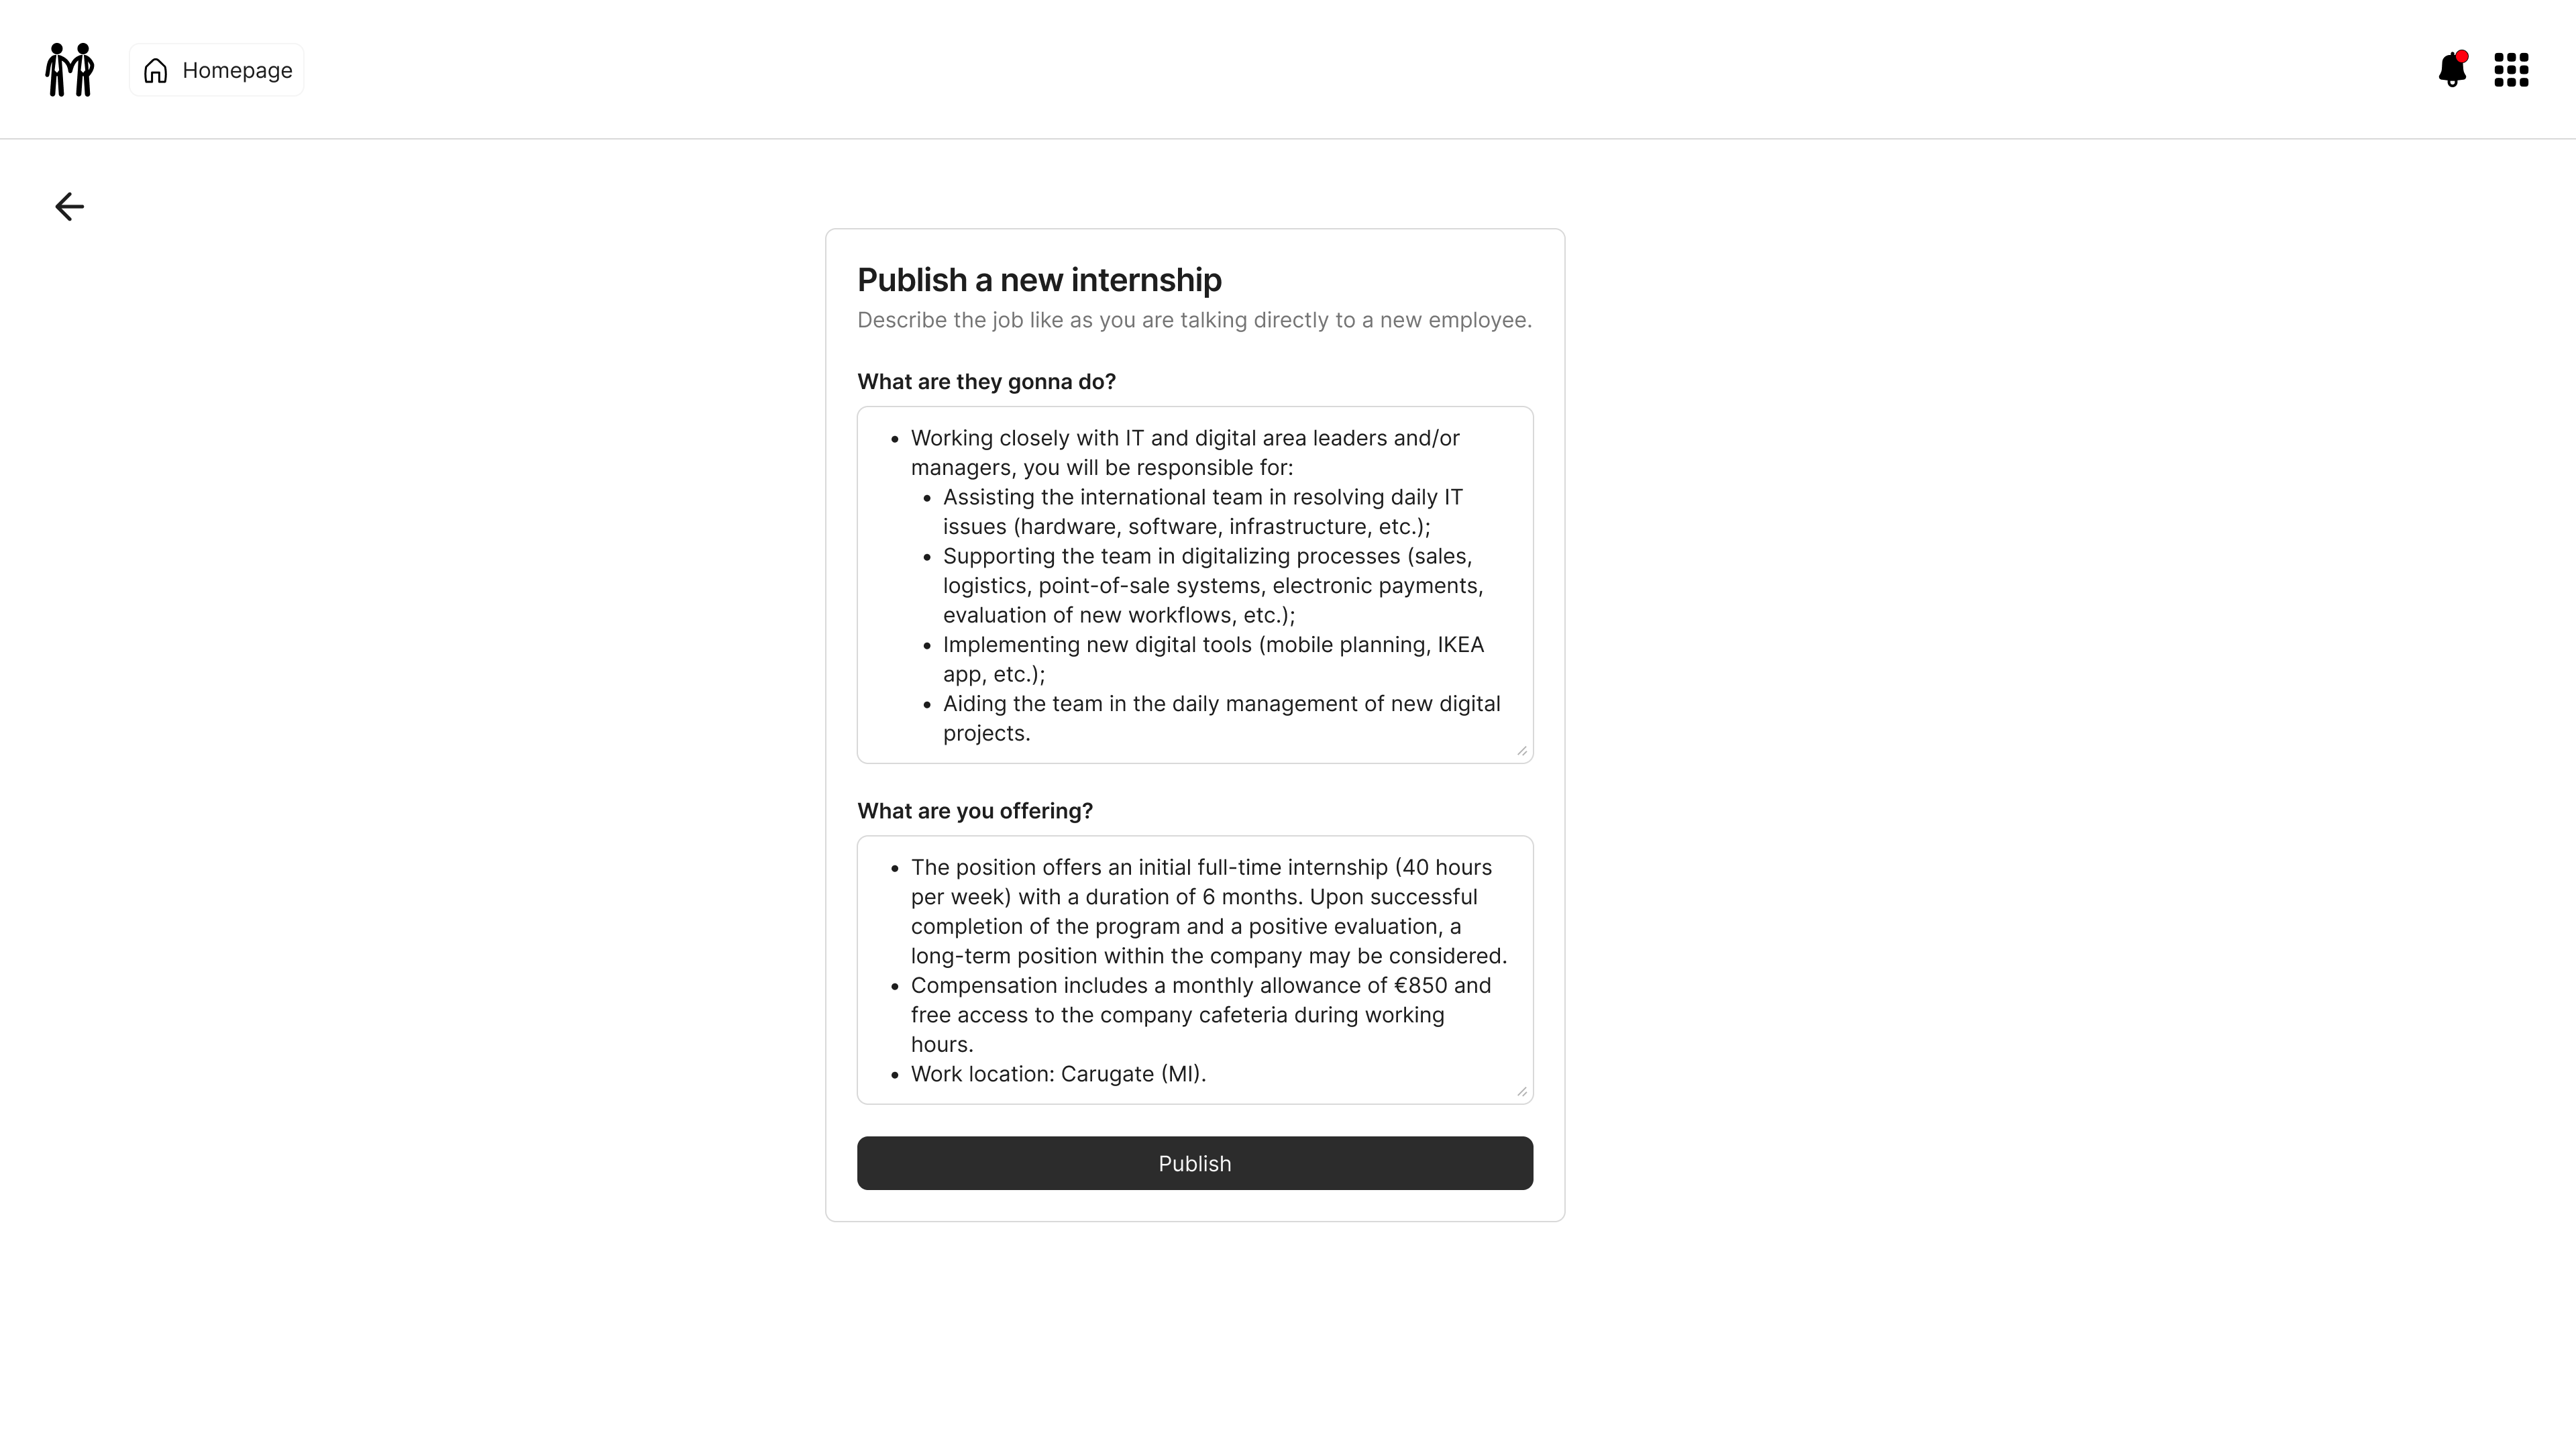
\includegraphics[width=1.0\textwidth]{Images/GUI/CO/Internship Creation - 2 - CO.png}}
    \caption{Internship Creation - 2 - CO}
    \label{fig:internship-creation-2-co}
\end{figure}

\par The Internship Creation page allows the CO to create a new internship. The CO is tasked to fill in all the
required information in order to post the internship on the platform.

\subsection{Internship Details - CO}
\label{subsec:internship-details-co}%

\begin{figure}[H]
    \centering
    \fbox{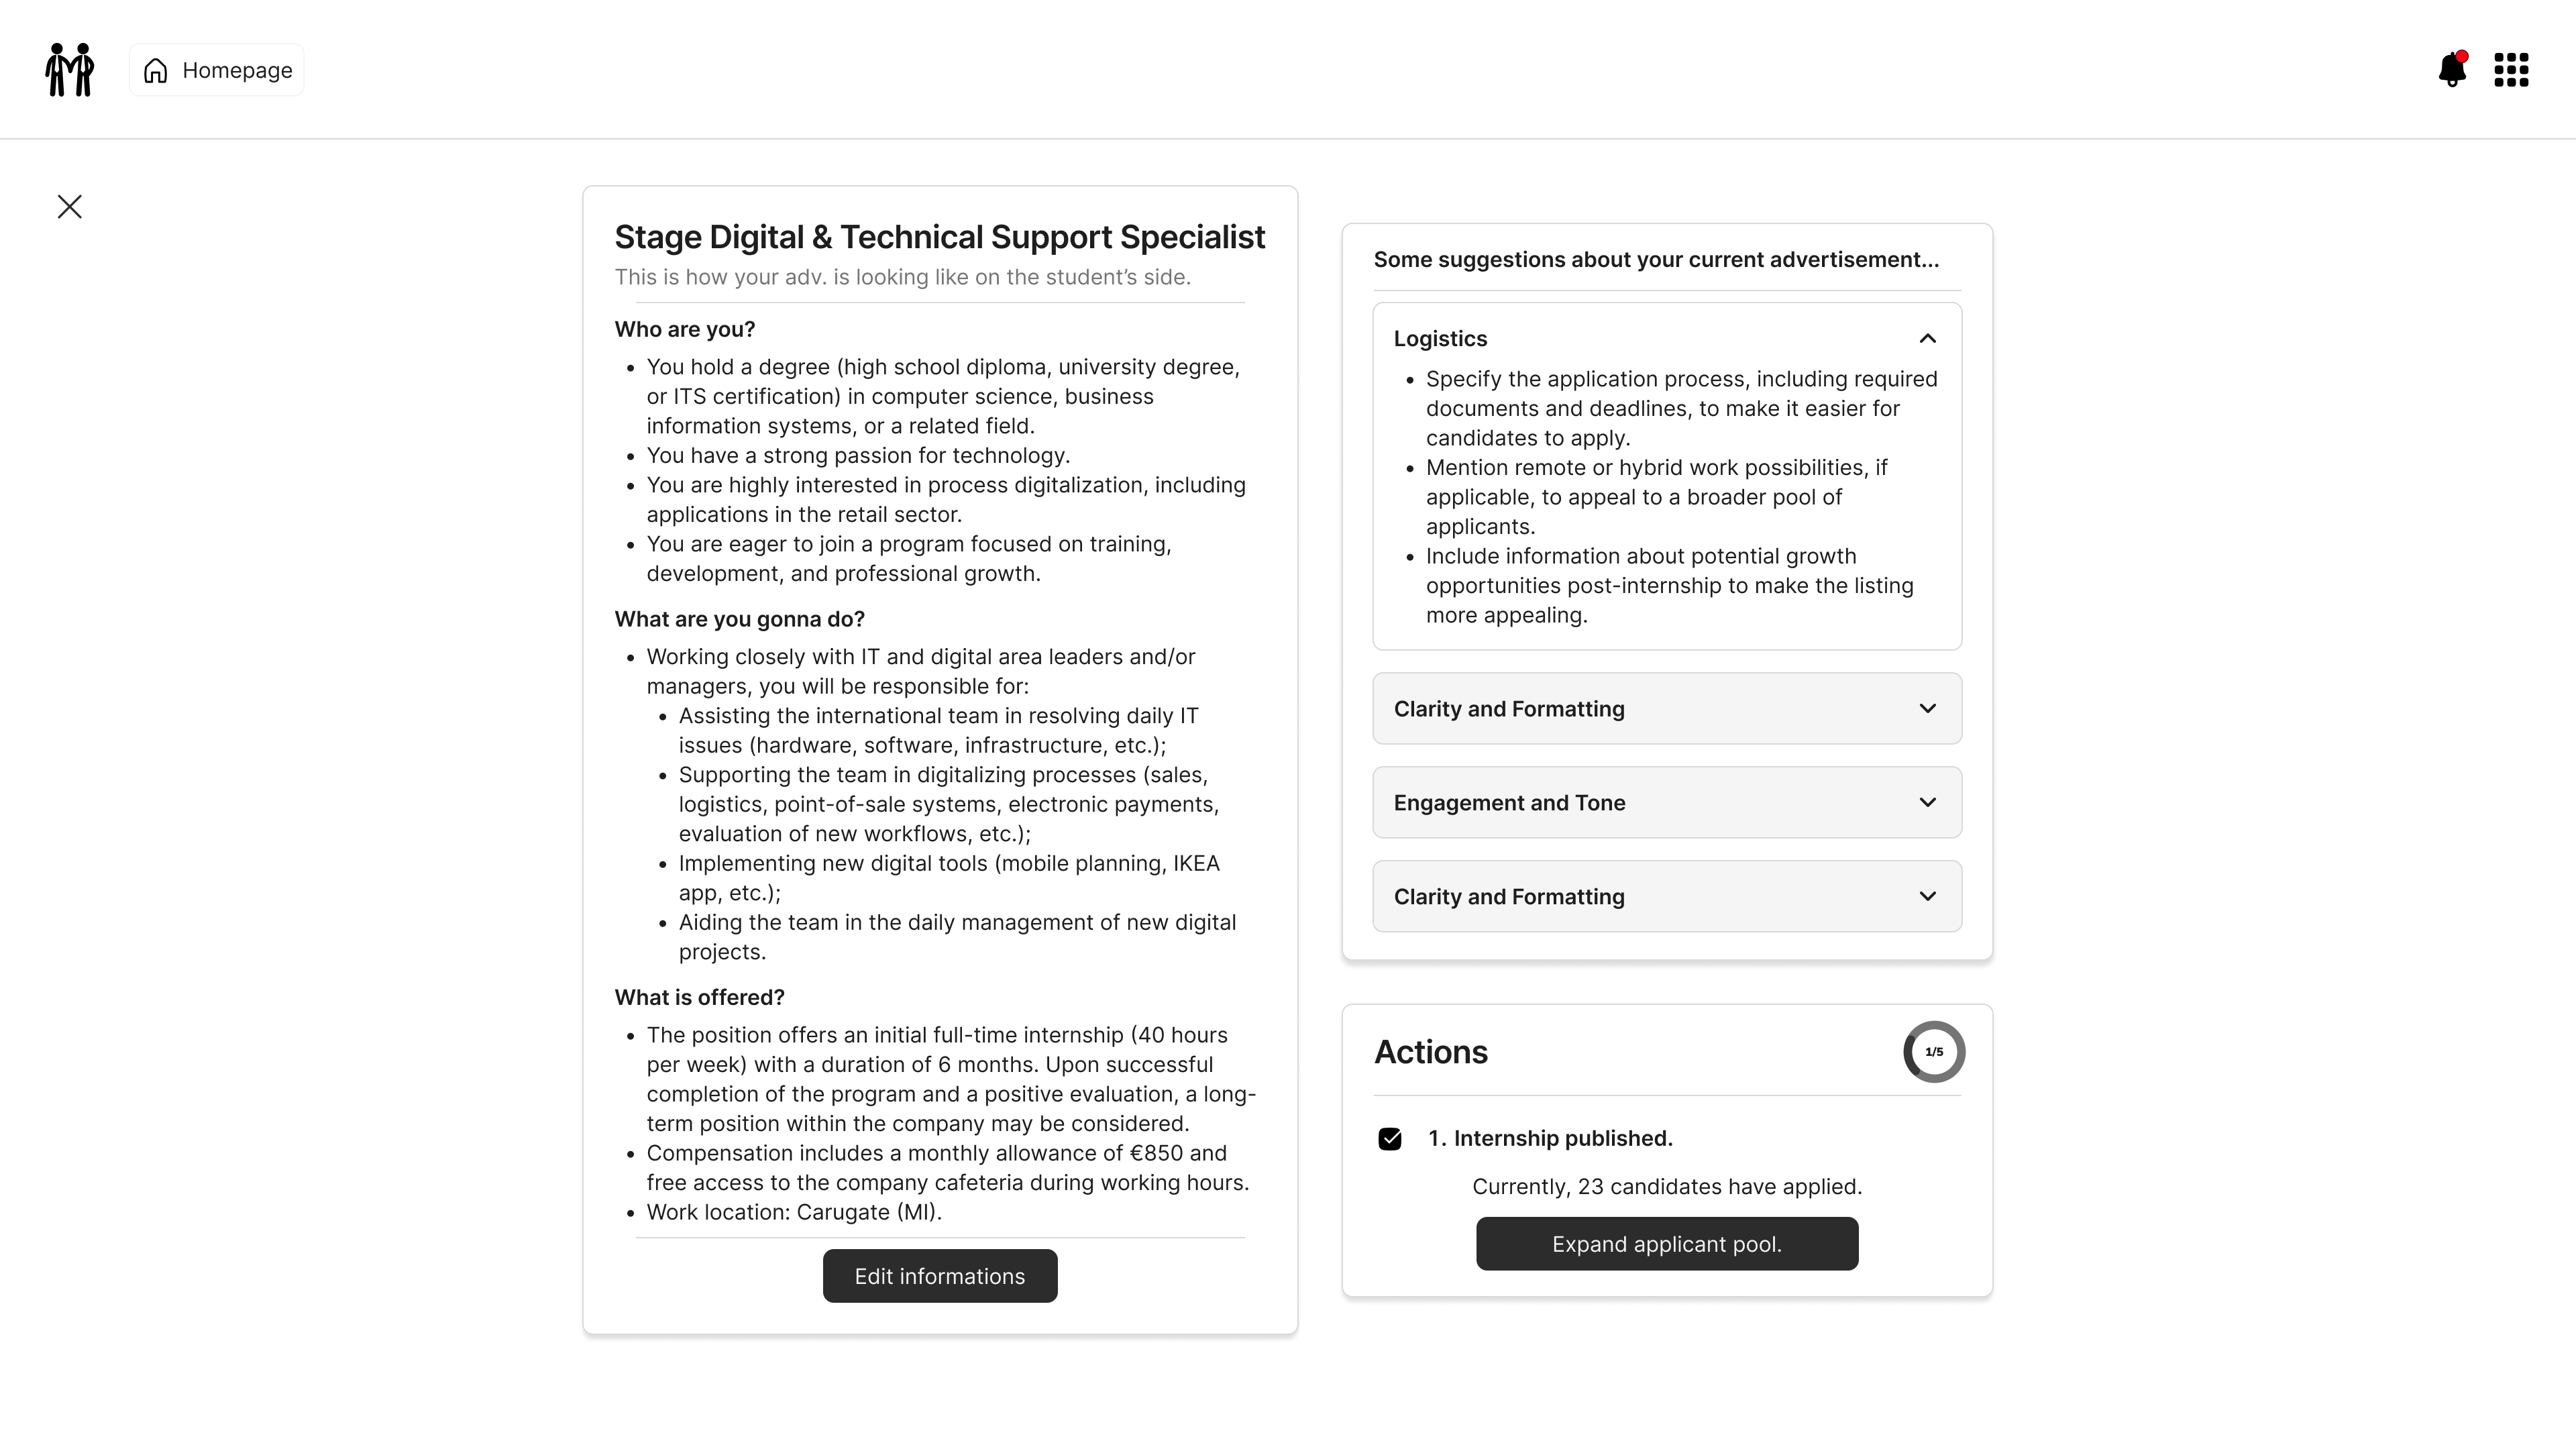
\includegraphics[width=1.0\textwidth]{Images/GUI/CO/Internship Published - Waiting for Applicants - CO.png}}
    \caption{Internship Details - 1 - CO}
    \label{fig:internship-creation-2-co}
\end{figure}

\par The Internship Details page will be presented in two critical stages divided by the application deadline. Before
the deadline the CO can not only edit the internship but also actively receive suggestions on how improve the
advertisement itself. After the deadline, the CO cannot edit the internship anymore in order to prevent abuse and
prevent confusion among the STs.

\par Also in this phase the CO can send notifications to the STs that the system has deemed as a good match for the
internship but have not applied yet. The CO can only view an anonymized version of the STs' profiles to prevent
information leakage. The interface used to select the STs will be shown later in the description of the "Request New
Applicants" page.

\begin{figure}[H]
    \centering
    \fbox{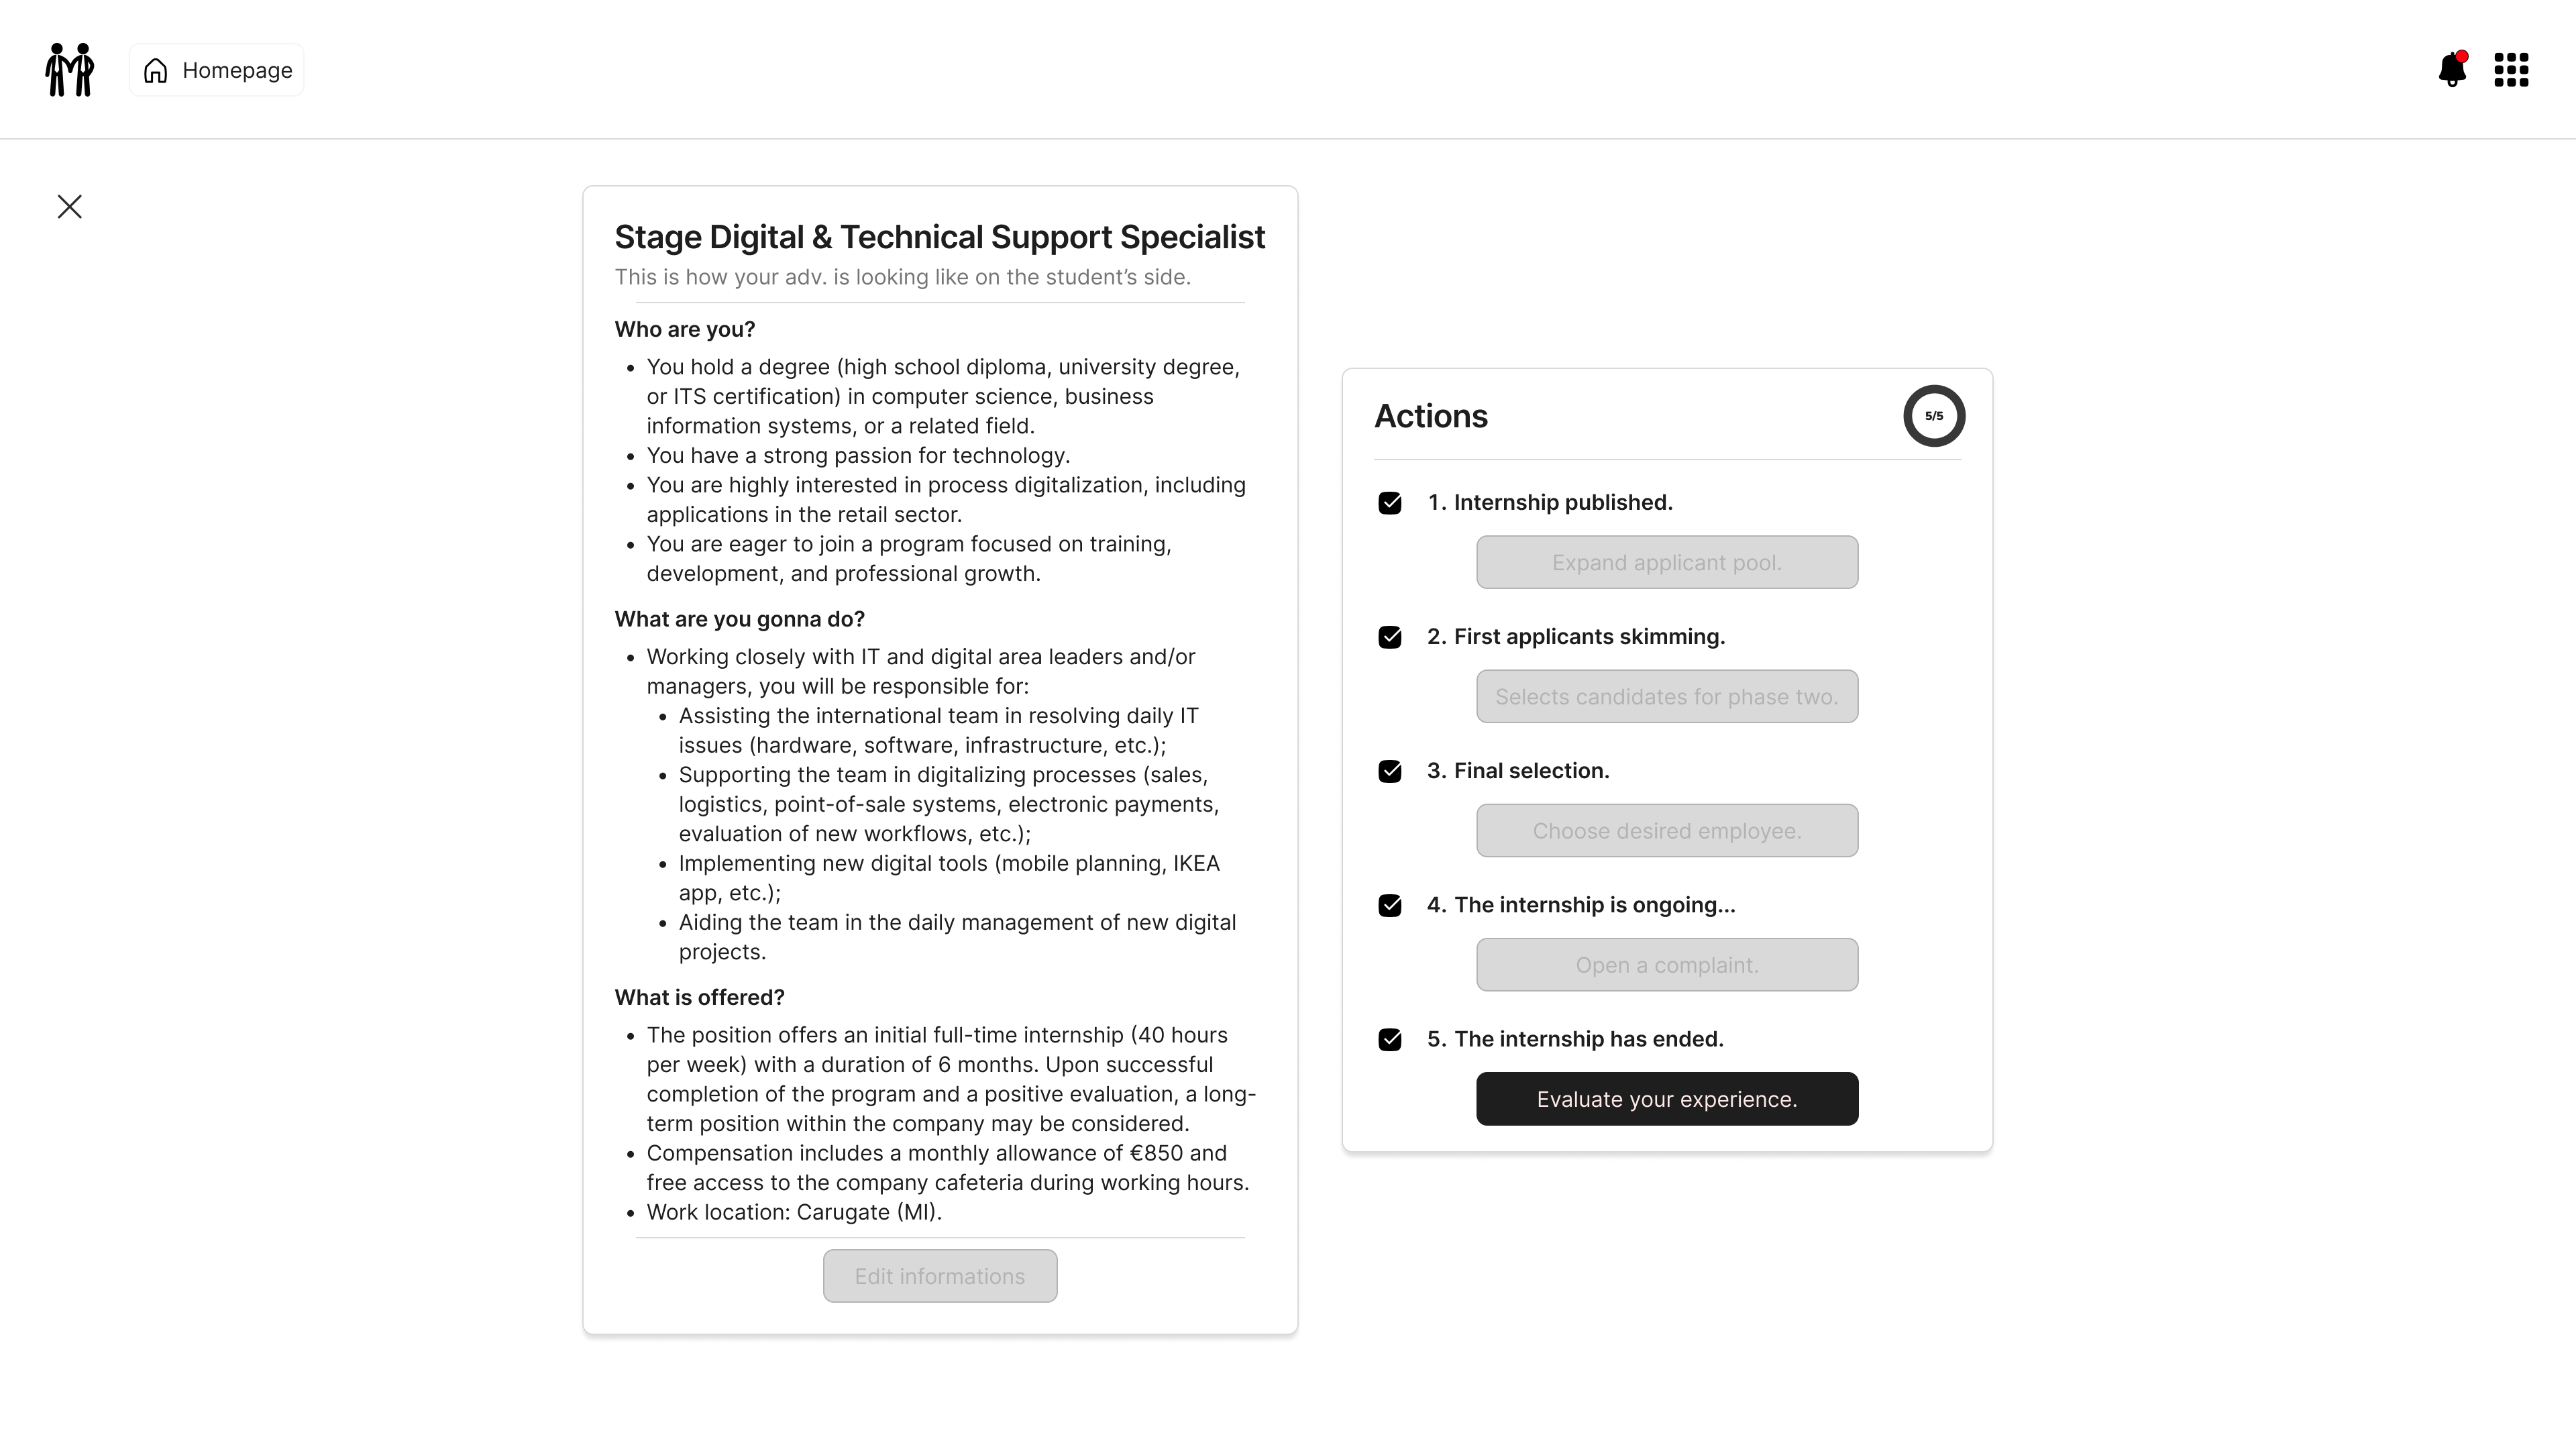
\includegraphics[width=1.0\textwidth]{Images/GUI/CO/Internship Published - Internship Completed - CO.png}}
    \caption{Internship Details - 1 - CO}
    \label{fig:internship-creation-2-co}
\end{figure}

\par As before, here is presented the page for a completed internship; the whole page evolution can easily be inferred
from this example.

\par Other that what has been already described, the CO can use this page - when appropriate - to request selected
STs to fill in the profiling questionnaire (Request Questionnaire), view the results of the questionnaire and select
the ST that will be hired (Select Employee), open a complaint if needed (Issue Reporting Form) and evaluate the
internship once it is over (Internship Feedback Survey).

\par The Internship Feedback Survey page and the Issue Reporting Form page are the same as the ones presented for the
ST and varies slightly only for the questions asked. For this reason, they will not be presented again.

\subsection{Request New Applicants - CO}
\label{subsec:request-new-applicants-co}%

\begin{figure}[H]
    \centering
    \fbox{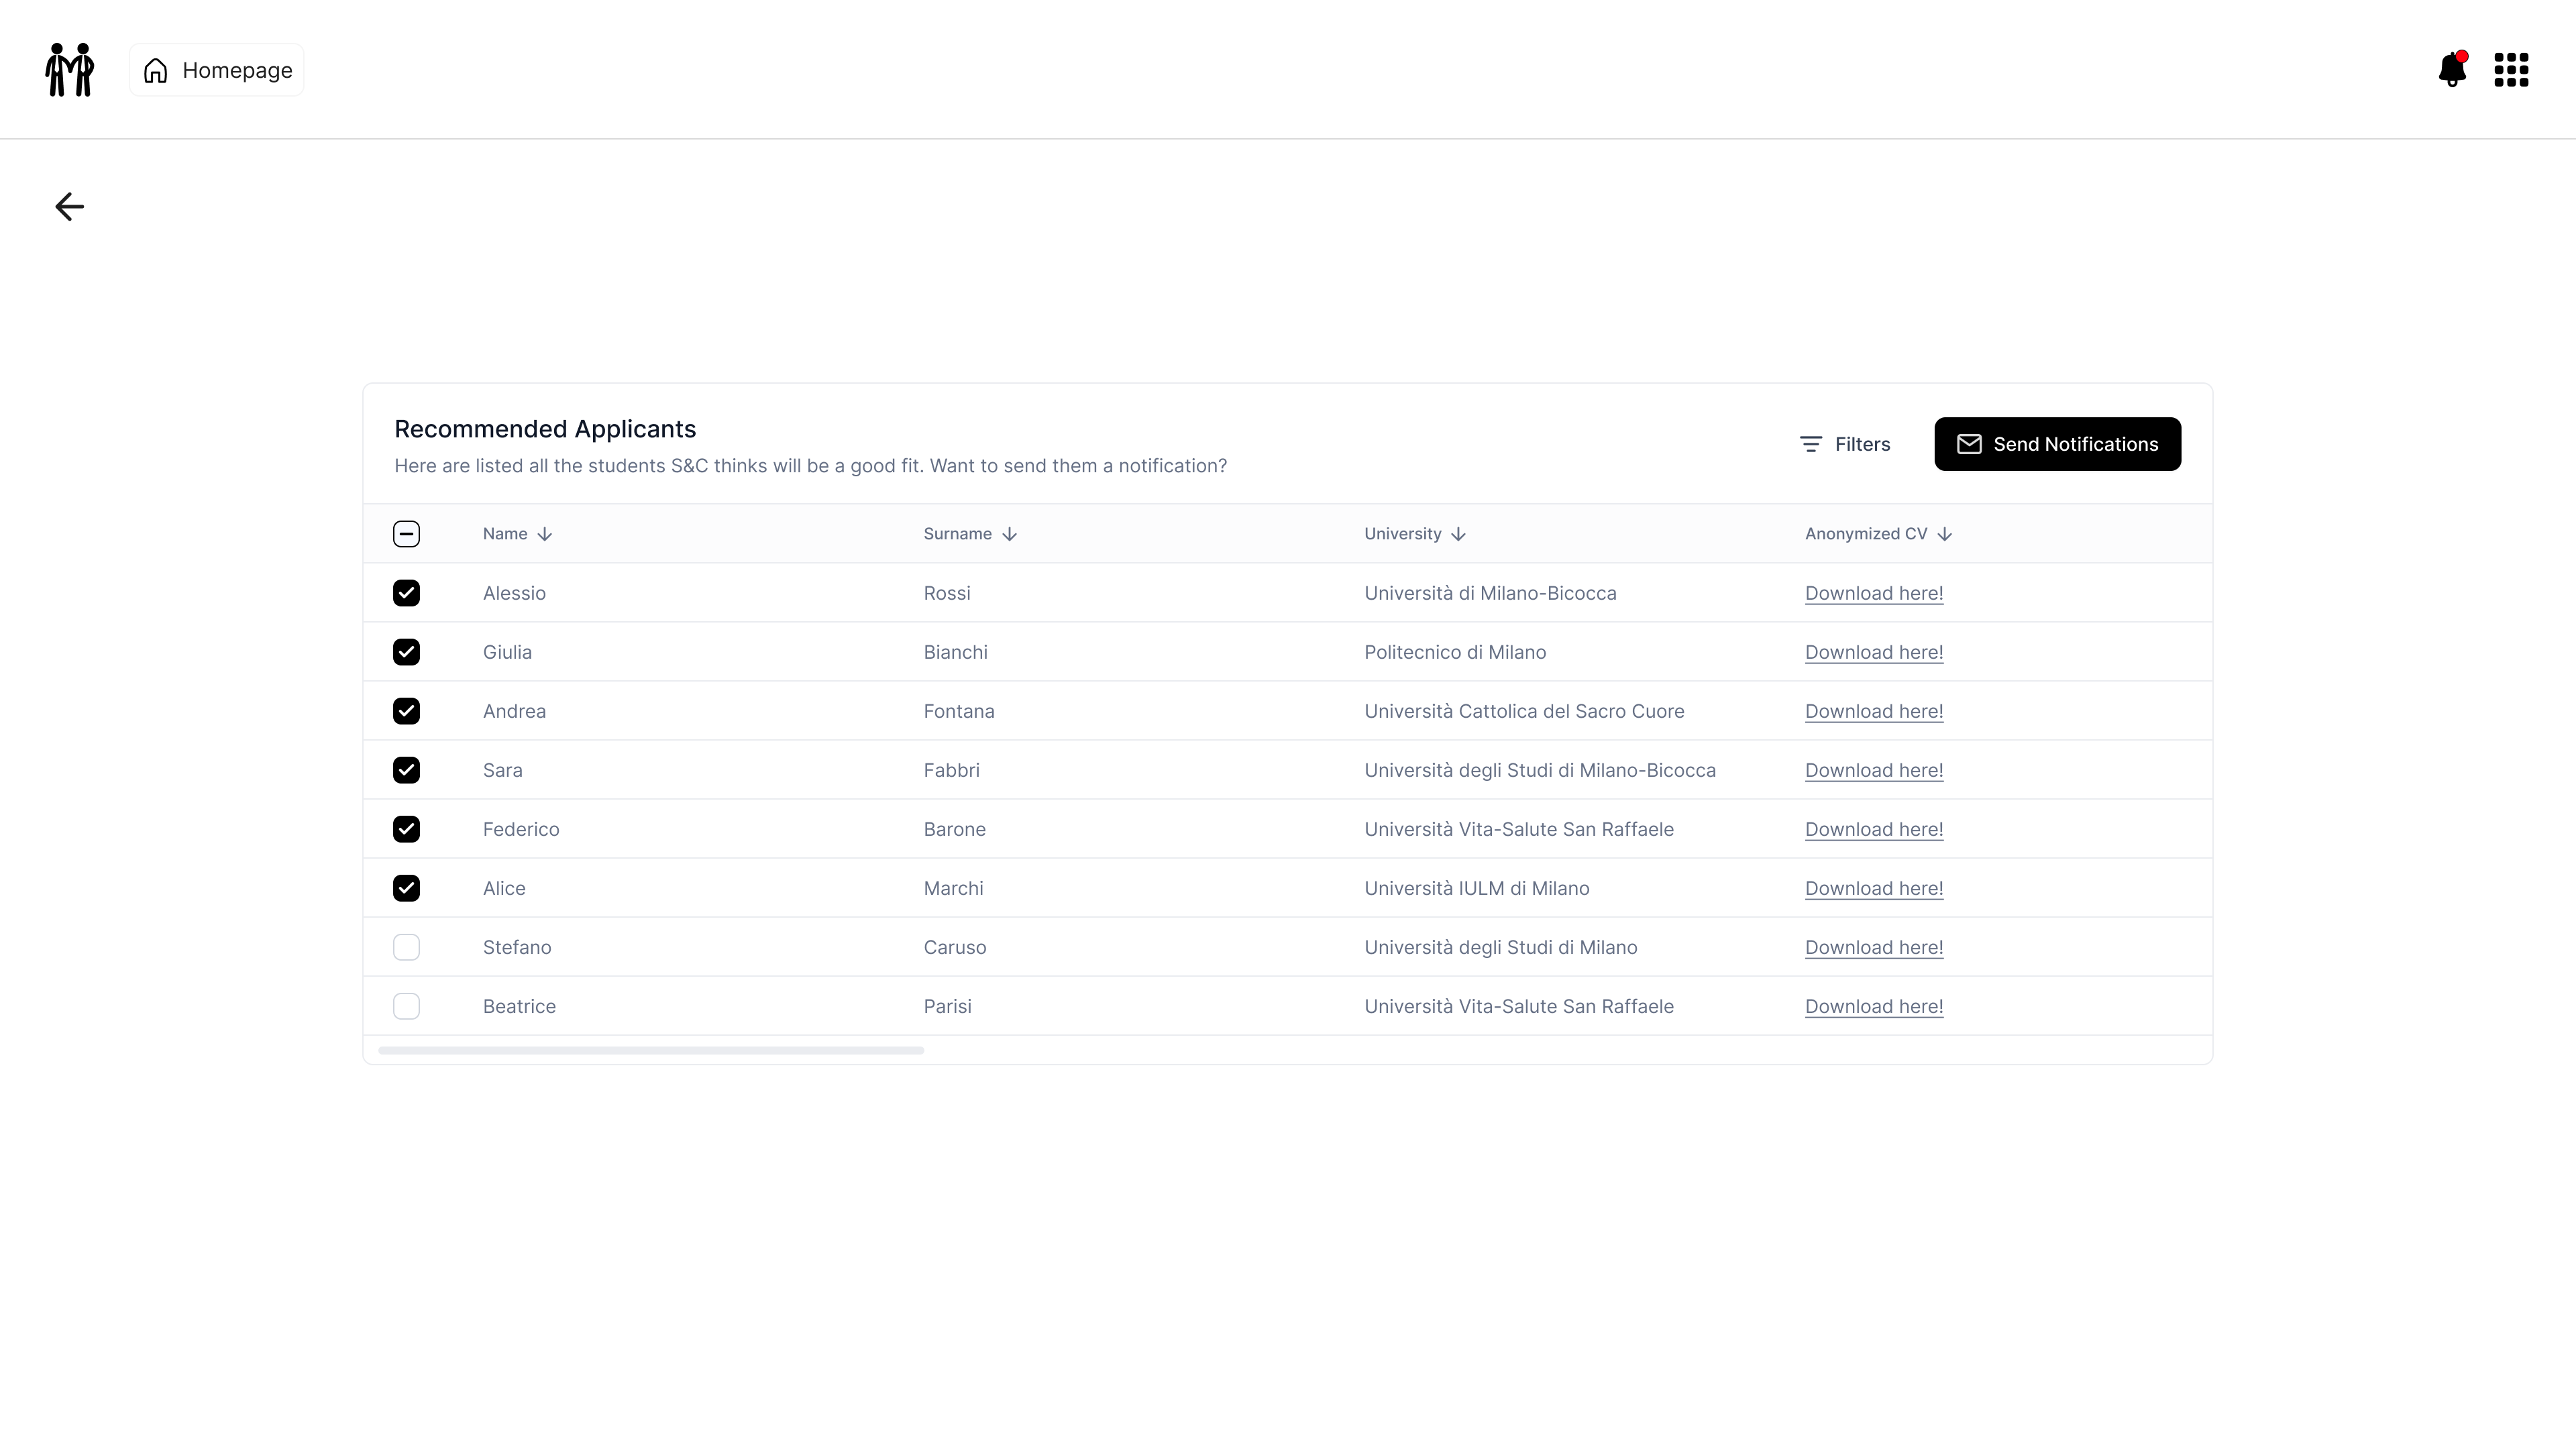
\includegraphics[width=1.0\textwidth]{Images/GUI/CO/Request New Applicants - CO.png}}
    \caption{Request New Applicants - CO}
    \label{fig:request-new-applicants-co}
\end{figure}

\par The Request New Applicants page allows the CO to send notifications to the STs that the system has deemed as a
good match for the internship but have not applied yet. These STs will maybe already have seen the internship thanks
to the system's suggestions but now we are showing them an active interest from the CO thus hoping to increase the
chances of them applying. The CO can only view an anonymized version of the STs' profiles to prevent information
leakage and abuse of the system: if the CO were able to see the full profiles of the STs, they could contact them
directly and bypass S\&C's system entirely.

\subsection{Request Questionnaire - CO}
\label{subsec:request-questionnaire-co}%

\begin{figure}[H]
    \centering
    \fbox{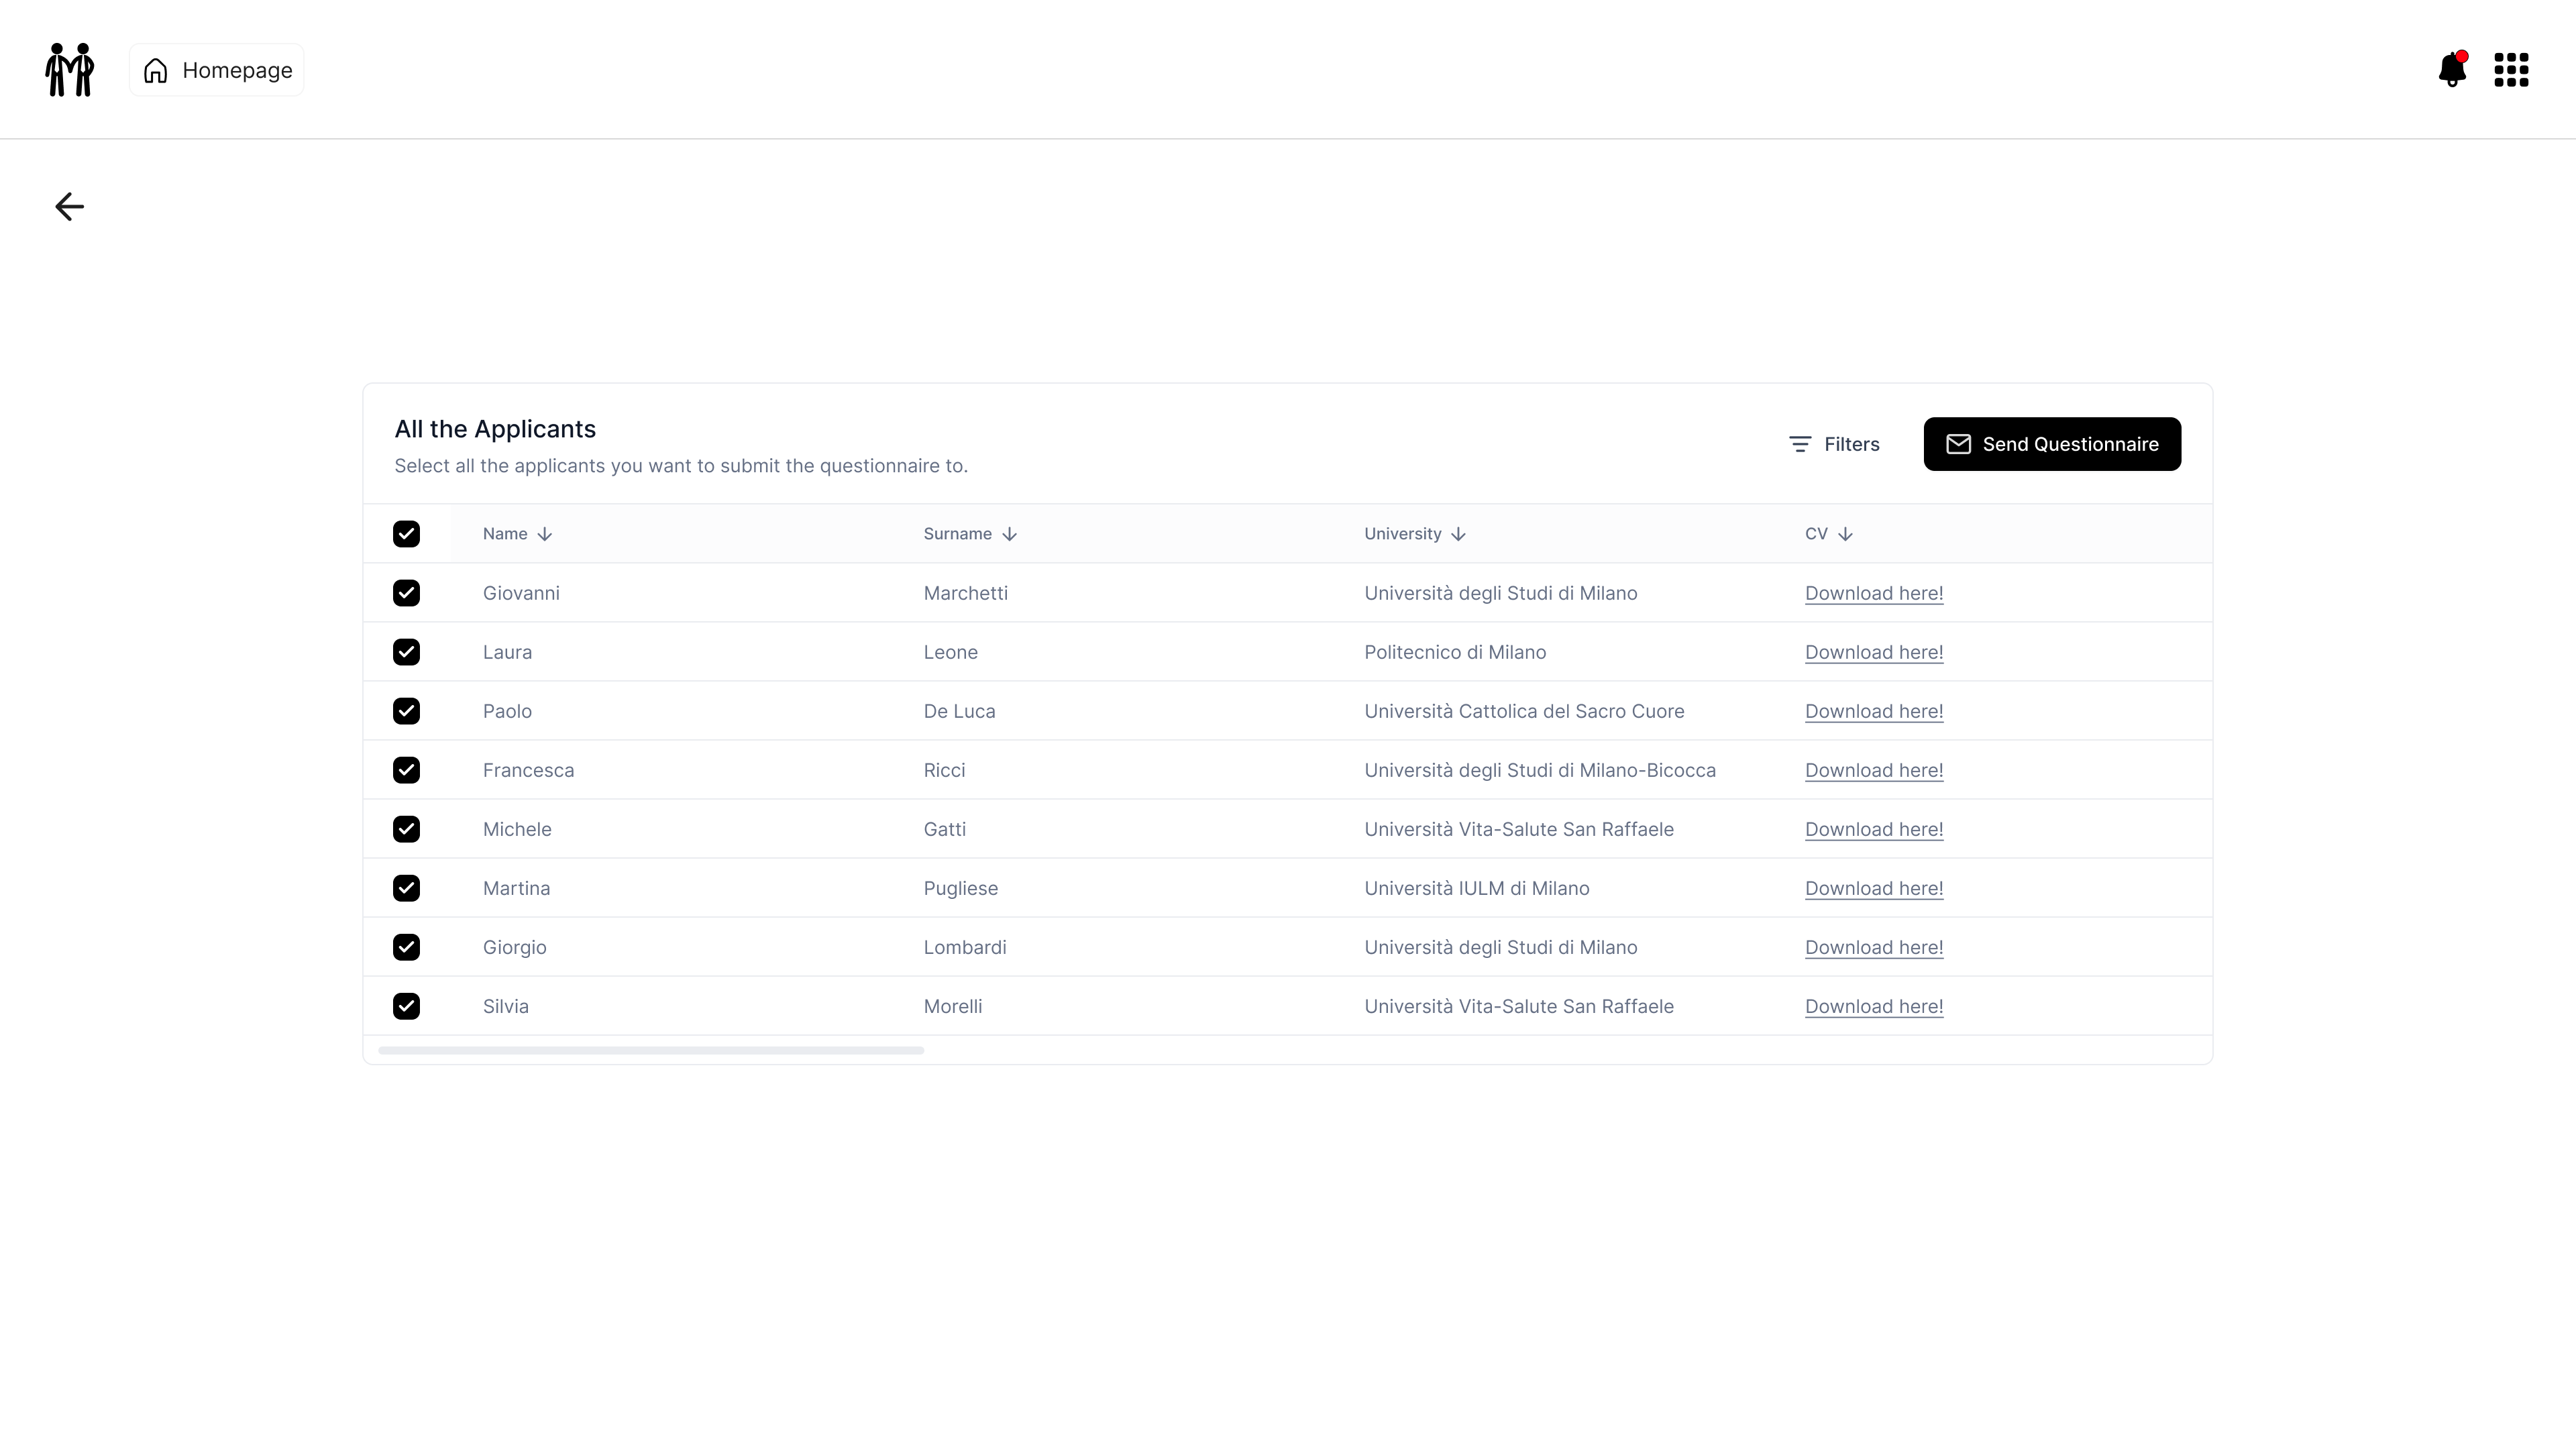
\includegraphics[width=1.0\textwidth]{Images/GUI/CO/Request Questionnaire - CO.png}}
    \caption{Request Questionnaire - CO}
    \label{fig:request-questionnaire-co}
\end{figure}

\par The Request Questionnaire page allows the CO to request the selected STs to fill in the profiling questionnaire.
Since the application deadline has passed - and the ST had already expressed their "consent" to be involved in this
internship - the CO can now see the full profiles of the STs.

\subsection{Select Employee - CO}
\label{subsec:select-employee-co}%

\begin{figure}[H]
    \centering
    \fbox{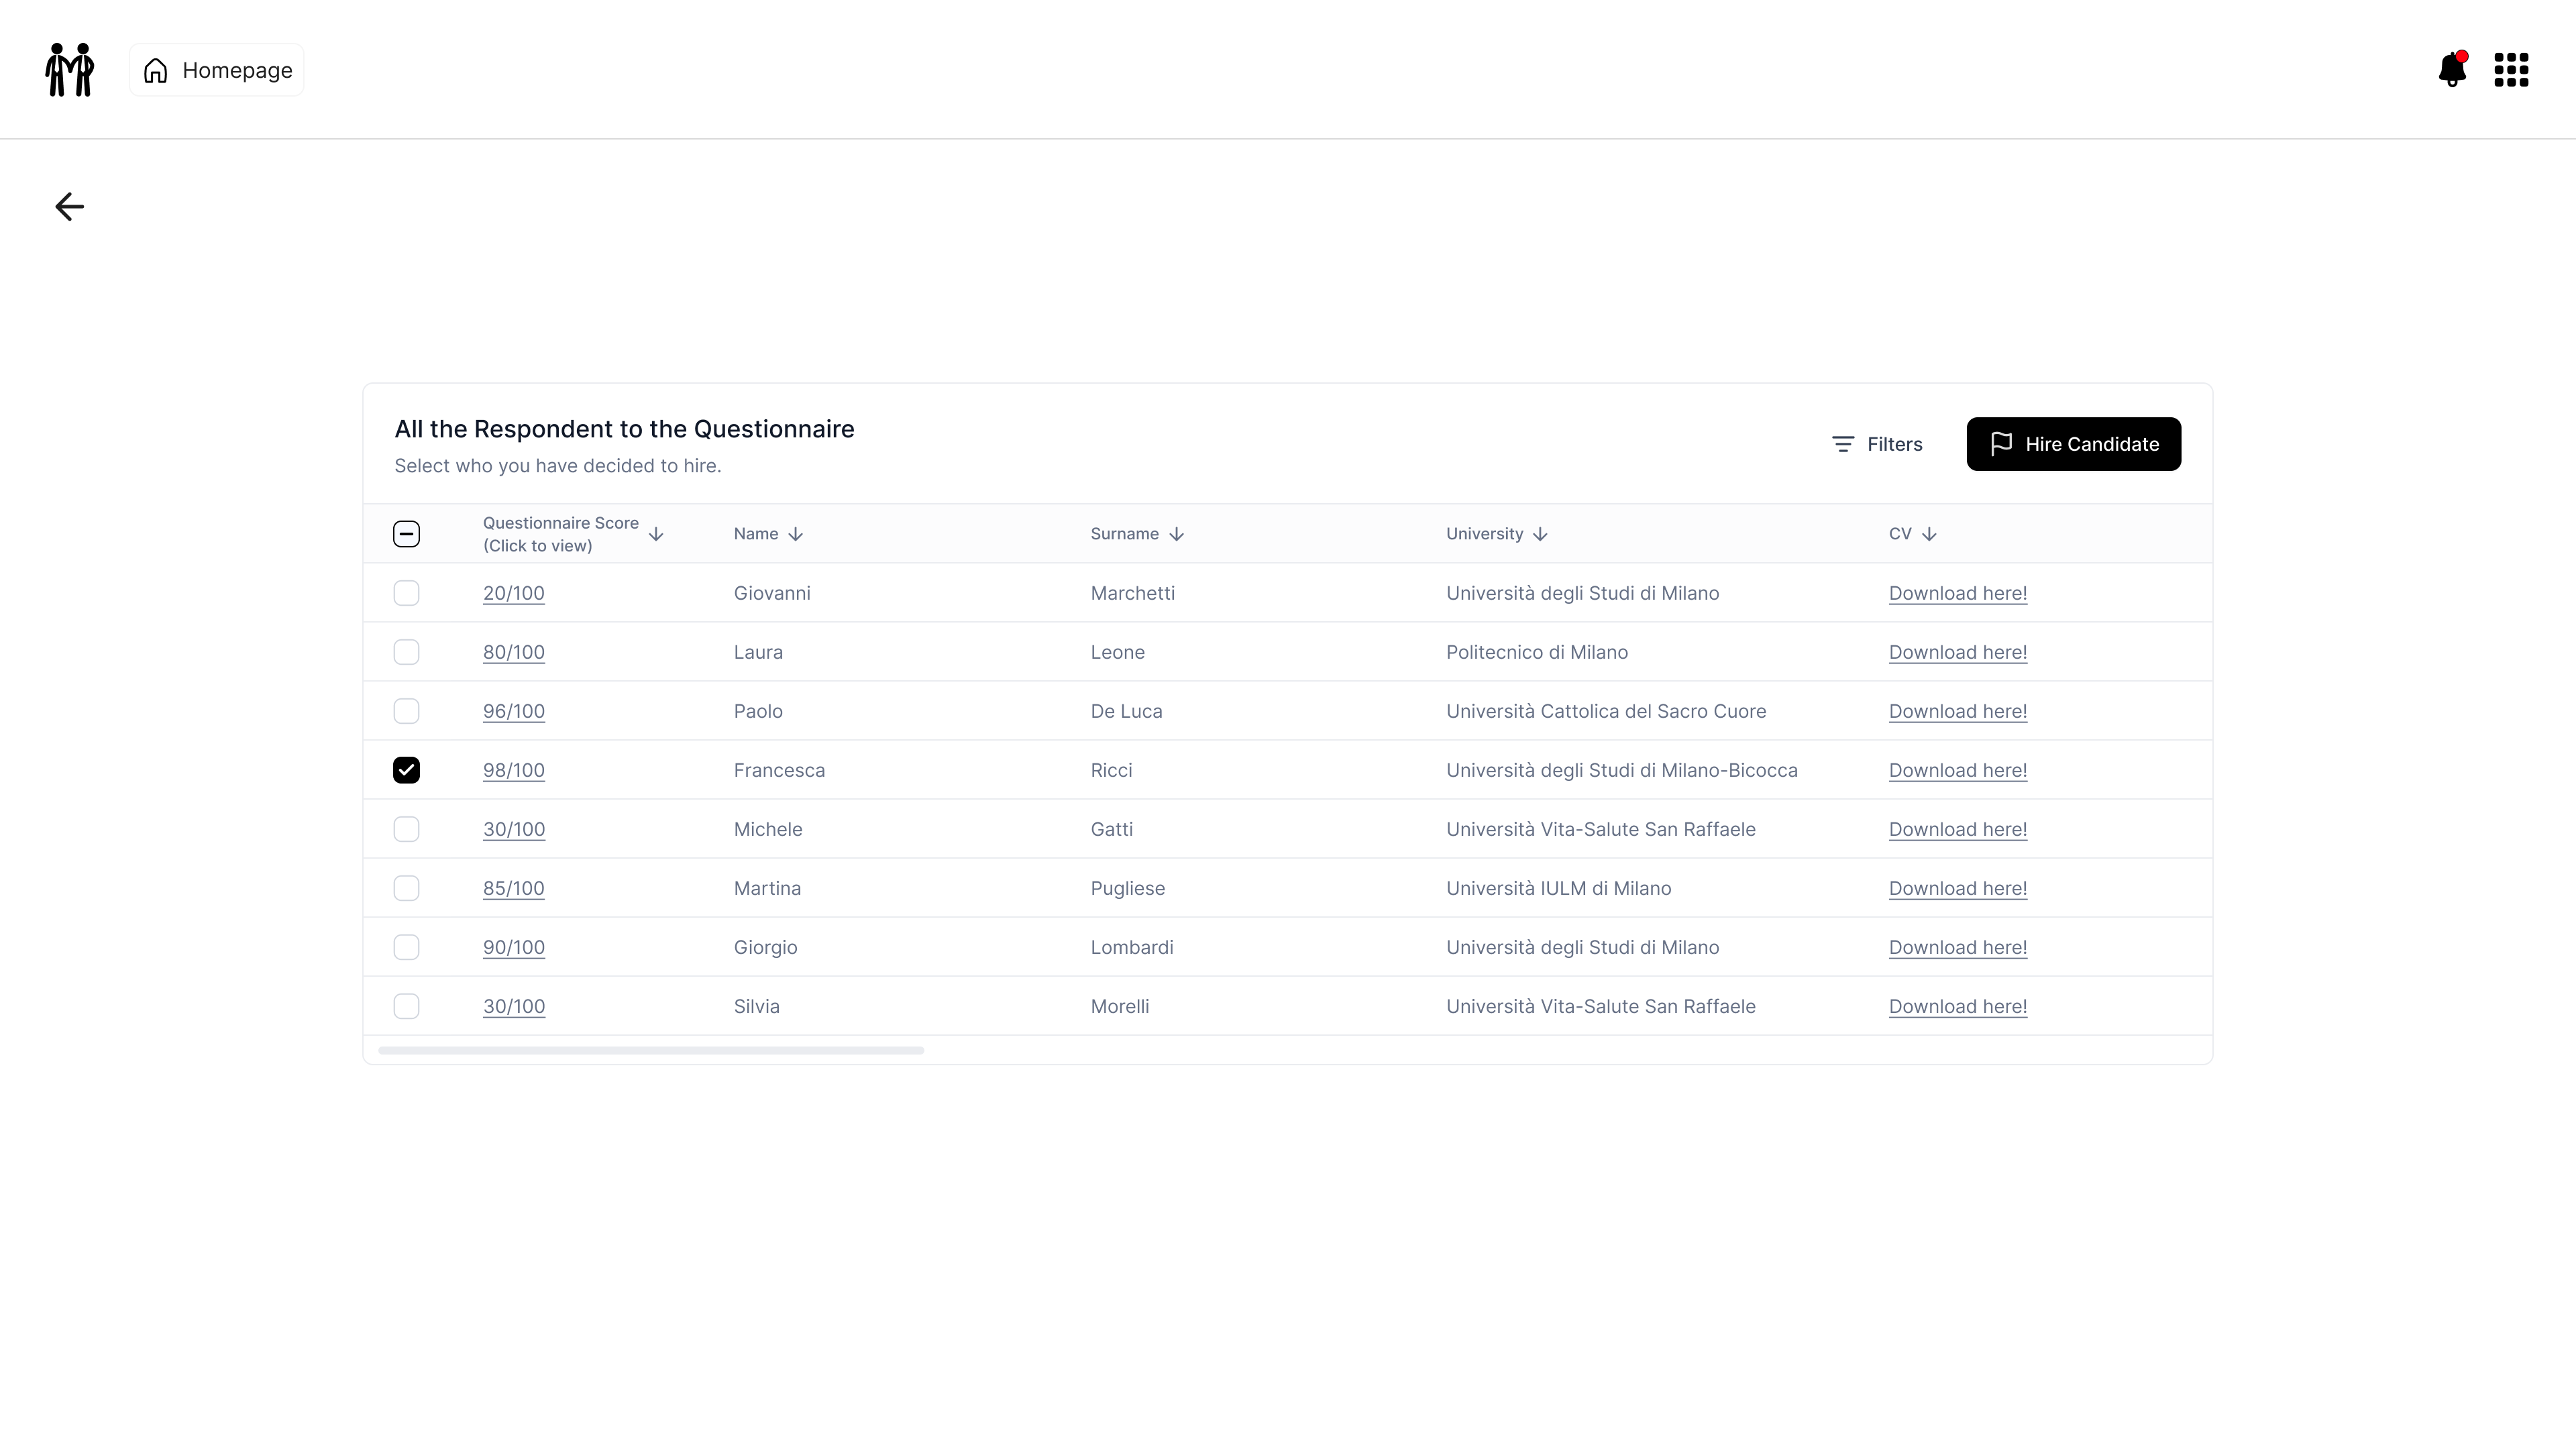
\includegraphics[width=1.0\textwidth]{Images/GUI/CO/Select Employee - CO.png}}
    \caption{Select Employee - CO}
    \label{fig:select-employee-co}
\end{figure}

\par The Select Employee page allows the CO to view the results of the questionnaire filled in by the STs and select
the ST that will be hired. This page is very similar to the Request Questionnaire page but with the addition of the
results of the questionnaire.

\section{"My Profile" - CO}
\label{subsec:profile-co}%

\begin{figure}[H]
    \centering
    \fbox{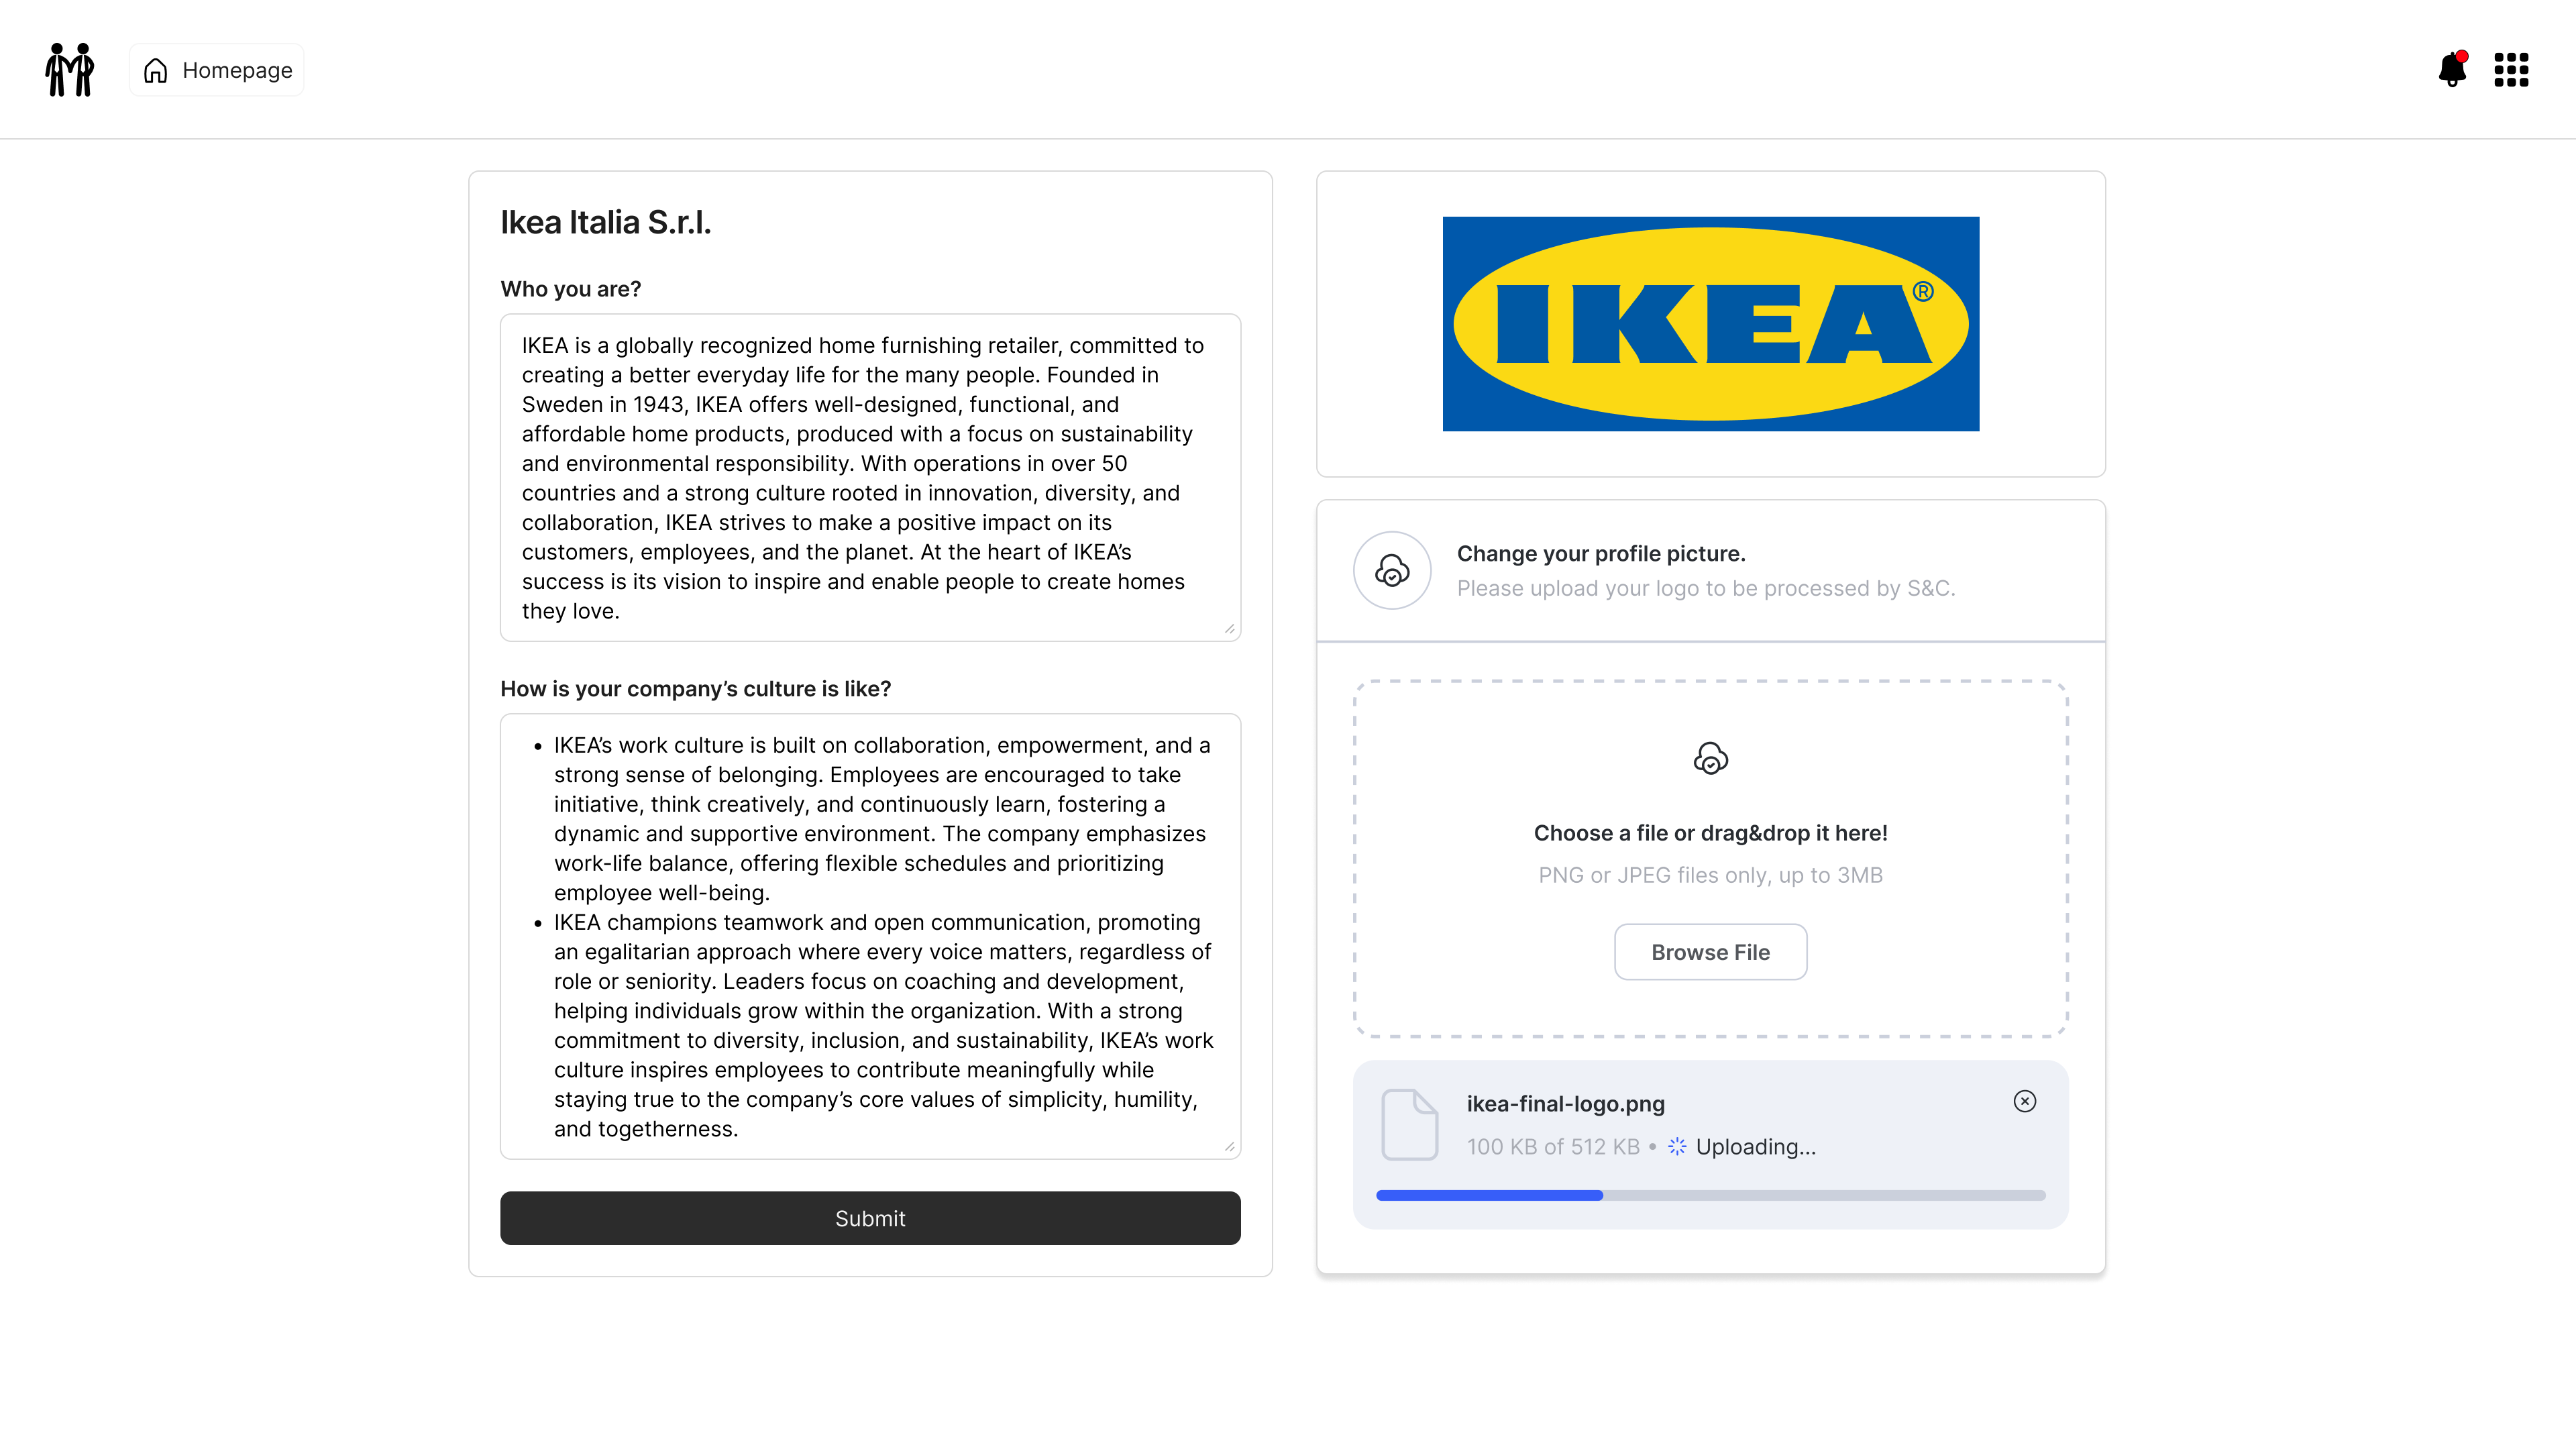
\includegraphics[width=1.0\textwidth]{Images/GUI/CO/Profile - CO.png}}
    \caption{"My Profile" - CO}
    \label{fig:profile-co}
\end{figure}

\par The "My Profile" page allows the CO to update their personal information. Along with the standard information,
this page offers the possibility to upload a the company's logo.


\chapter{Requirements Traceability}
\label{ch:requirements-traceability}
\par In this section, we aim to establish a clear mapping between the components previously described and the requirements they fulfill.
Keeping track of which requirements a component should satisfy is crucial ot ensure that the final product meets the initial specifications.
The considered requirements can be found in the associated RASD document.
\begin{itemize}
    \item \textbf{Login Manager:}
          \begin{itemize}
              \item R01
              \item R04
              \item R05
              \item R06
              \item R07
          \end{itemize}
    \item \textbf{Internship Manager:}
          \begin{itemize}
              \item R11
              \item R14
              \item R15
              \item R16
              \item R22
              \item R23
              \item R25
              \item R27
              \item R28
              \item R29
              \item R33
              \item R36
              \item R37
              \item R39
              \item R43
          \end{itemize}
    \item \textbf{Profile Manager:}
          \begin{itemize}
              \item R08
              \item R15
              \item R25
              \item R39
              \item R40
          \end{itemize}
    \item \textbf{Questionnaire Manager:}
          \begin{itemize}
              \item R18
              \item R21
              \item R26
              \item R32
          \end{itemize}
    \item \textbf{Complaint Manager:}
          \begin{itemize}
              \item R19
              \item R30
              \item R34
              \item R37
          \end{itemize}
    \item \textbf{Notification Manager:}
          \begin{itemize}
              \item R13
              \item R17
              \item R20
              \item R31
              \item R35
              \item R38
              \item R42
              \item R43
          \end{itemize}
    \item \textbf{Recommendation Manager:}
          \begin{itemize}
              \item R11
              \item R12
              \item R41
              \item R42
          \end{itemize}
    \item \textbf{Suggestion Manager:}
          \begin{itemize}
              \item R09
              \item R24
          \end{itemize}
    \item \textbf{Dashboard Manager:}
          \begin{itemize}
              \item R10
              \item R11
              \item R14
              \item R36
                    % The notifications can be displayed in the dashboard if they happen when the web application is open
              \item R13
              \item R17
              \item R20
              \item R31
              \item R35
              \item R38
              \item R42
          \end{itemize}
    \item \textbf{Query Manager:}
          \begin{itemize}
              \item R02
              \item R03
              \item R06
              \item R08
              \item R26
              \item R40
          \end{itemize}
\end{itemize}

\end{document}